\ifx\wholebook\relax \else
\documentclass[b5paper]{ctexart}
\usepackage[nomarginpar
  %, margin=.5in
]{geometry}

\addtolength{\oddsidemargin}{-0.05in}
\addtolength{\evensidemargin}{-0.05in}
\addtolength{\textwidth}{0.1in}
\usepackage[cn]{../prelude}

\setcounter{page}{1}

\begin{document}

\title{搜索}

\author{刘新宇
\thanks{{\bfseries 刘新宇 } \newline
  Email: liuxinyu95@gmail.com \newline}
  }

\maketitle
\fi

\markboth{搜索}{基本算法}

\ifx\wholebook\relax
\chapter{搜索}
\numberwithin{Exercise}{chapter}
\fi

\def\includetikz{}

现代计算机系统使很多困难的搜索问题得以实现。工业机器人可以从堆在生产线旁的零件中找出正确的进行组装,带有卫星导航系统的汽车可以在地图中找到前往目的地的最佳路线,智能手机还能搜索出最便宜的购物方案。本章介绍最基本的查找、匹配、图搜索算法。

\section{$k$选择问题}
\index{$k$选择}

这一问题是说如何在$n$个元素中寻找第$k$大(或小)的元素。这里大小的含义是抽象的序关系。我们先用$\leq$关系找出第$k$小的元素,然后再推广到其它一般情况。最简单的方法是先找到最小的,然后在剩余元素中寻找第二小的。进行$k$次就可以找到第$k$小的元素。在$n$个元素中寻找最小元素是线性时间$O(n)$的。因此总时间为$O(kn)$。我们也可以利用堆。这样可以在$O(\lg n)$时间内更新、获取顶部,重复$k$次可以在$O(k \lg n)$时间内获得答案。

\be
top\ k\ xs = find\ k\ (\textit{heapify}\ xs)
\ee

或写成柯里化形式:

\be
top\ k\ = (find\ k) \circ \textit{heapify}
\label{eq:kth-heap1}
\ee

其中:

\be
\begin{array}{rcl}
find\ 0 & = & top \\
find\ k & = & (find\ (k - 1)) \circ pop
\end{array}
\label{eq:kth-heap2}
\ee

我们还能找到更好的方法。使用分治策略将元素划分为$A$、$B$,使得$A$中元素都不大于($\leq$)$B$中元素。令$m = |A|$为$A$的大小,比较$m$和$k$:

\begin{enumerate}
\item 若$k < m$,则第$k$小的元素在$A$中,我们丢弃$B$,然后在$A$中递归查找;
\item 若$m < k$,则第$k$小的元素在$B$中,我们丢弃$A$,然后在$B$中递归查找第$(k-m)$小的元素。
\end{enumerate}

理想情况下划分是平衡的,$A$、$B$大小相当,每次问题规模减半,复杂度为$O(n + n/2 + n/4 +...) = O(n)$。我们利用上一章快速排序中的划分方法\textit{part},随机选择一个元素(如第一个)作为基准$p$。将所有$\leq p$的元素放入$A$,剩余元素放入$B$。这样若$m = k - 1$,则$p$就是第$k$小的元素,否则我们递归在$A$或$B$中查找。

\be
top\ k\ (x \cons xs) = \begin{cases}
  m = k - 1: & x, \text{其中}: m = |A|, (A, B) = part\ (\leq x)\ xs \\
  m < k - 1: & top\ (k - m - 1)\ B \\
  \text{否则}: & top\ k\ A \\
\end{cases}
\ee

和快速排序一样,最差情况下划分结果总不平衡,性能退化为$O(kn)$或$O((n-k)n)$。平均情况下可以在线性时间内找到答案。我们也可以应用快速排序划分中各种改进,如三点中值法\footnote{Blum、Floyd、Pratt、Rivest和Tarjan在1973年给出了一个线性时间方法\cite{CLRS}\cite{median-of-median}。将列表划分为若干组,每组最多5个元素,总共选出$n/5$个中值。重复这一步骤选出中值的中值。}和随机划分法:

\begin{algorithmic}[1]
\Function{Top}{$k, A, l, u$}
  \State \textproc{Exchange} $A[l] \leftrightarrow A[$ \Call{Random}{$l, u$} $]$ \Comment{随机在$[l, u]$内选择}
  \State $p \gets$ \Call{Partition}{$A, l, u$}
  \If{$p - l + 1 = k$}
    \State \Return $A[p]$
  \EndIf
  \If{$k < p - l + 1$}
    \State \Return \Call{Top}{$k, A, l, p-1$}
  \EndIf
  \State \Return \Call{Top}{$k - p + l - 1, A, p + 1, u$}
\EndFunction
\end{algorithmic}

我们可以调整这一方法获取全部的前$k$个值($k$个值间的顺序是任意的),如下面的例子程序:

\lstset{frame = single}
\begin{Haskell}
tops _ [] = []
tops 0 _  = []
tops n (x:xs) | len == n = as
              | len <  n = as ++ [x] ++ tops (n - len - 1) bs
              | otherwise = tops n as
    where
      (as, bs) = partition (<= x) xs
      len = length as
\end{Haskell}

\section{二分查找}
\index{二分查找}

中学时候老师表演过一个“数学魔术”:学生随便想一个1000以内的数,老师问十个问题,学生回答是或否。然后老师就能猜出这个数。例如:是偶数么?是素数么?所有位上的数字都相同么?能被3整除么?等等。神奇的是,老师总能猜到答案。在1000以内,如果每次通过问答排除一半数字,10次内就能找出答案。因为$2^{10} = 1024 > 1000$。“是偶数么?”就是一个非常好的问题,它能去掉一半的数字\footnote{社交网络上曾有一个“读心术”游戏。玩家暗想世界上任何一个人,人工智能机器人提16个问题,玩家回答是或否,最后机器人能说出玩家暗想的人是谁。}。设计奇偶性这样的问题需要一定的技巧,但存在着简单的方法每次淘汰掉一半。我们经常在电视里看到这样的竞猜节目。主持人展示一件商品,然后让观众猜价格。并告之是猜高了还是低了。如果能够在30秒内猜对,就获得奖励。例如:1000元,高了;500元,低了;750元,低了;890元,低了;990元,正确!这位观众使用了“二分查找”策略。为了在已序序列$A$中寻找$x$,我们找到位于序列中点上的$y$,和$x$比较。如果$x = y$,查找结束;如果$x < y$,由于$A$是已序的,我们只需要在前半部分继续查找;否则在后半部分查找。这样不断缩小$A$的规模,如果当$A = []$时仍未找到,则$x$不存在。二分查找要求$A$是已序的,我曾经看到有人试图对未排序的数组二分查找,深陷其中却得不到答案。高德纳说:“虽然二分查找的基本思想相对直观,具体细节却复杂得不可思议……”。本特利发现大多数二分查找的实现中含有错误。有趣的是他本人在《编程珠玑》第一版中给出的实现也包含了一个错误,直到20多年后才被发现\cite{Bentley}。下面给出了二分查找的实现,令数组$A$的上下界为$l$、$u$(不含$u$)。

\be
\textit{bsearch}\ x\ A\ (l, u) = \begin{cases}
  u < l: & \textit{Nothing} \\
  x = A[m]: & m, \text{其中}: m =  l + \lfloor \dfrac{u - l}{2} \rfloor \\
  x < A[m]: & \textit{bsearch}\ x\ A\ (l, m - 1) \\
  \text{否则}: & \textit{bsearch}\ x\ A\ (m + 1, u) \\
\end{cases}
\ee

我们也可以消除递归,通过更新边界实现二分查找:

\begin{algorithmic}[1]
\Function{Binary-Search}{$x, A, l, u$}
  \While{$l < u$}
    \State $m \gets l + \lfloor \dfrac{u - l}{2} \rfloor$ \Comment{避免$\lfloor \dfrac{l+u}{2} \rfloor$溢出}
    \If{$A[m] = x$}
      \State \Return $m$
    \EndIf
    \If{$x < A[m]$}
      \State $u \gets m - 1$
    \Else
      \State $l \gets m + 1$
    \EndIf
  \EndWhile
  \State Not found
\EndFunction
\end{algorithmic}

由于每次将数组减半,二分查找的复杂度为$O(\lg n)$。二分查找还可以搜索单调函数的解。例如方程$a^x = y$,其中$a \leq y$,$a$、$y$都是自然数,我们寻找$x$的整数解。我们可以穷举:从0开始依次尝试$a^0, a^1, a^2, ...$,直到发现某个$a^i = y$,或者$a^i < y < a^{i+1}$,表示方程无整数解。对很大的$a$和$x$,如果需要保持精度,则计算$a^x$会消耗一定的时间\footnote{当然,我们可以复用$a^n$的结果来计算$a^{n+1} = a a^n$。这里我们考虑一般意义下的单调函数$f(n)$。}。我们可以用二分查找来进行改进。首先估计解的上限。由于$a^y \geq y$,我们可以在区间$[0, 1, ..., y]$内搜索。由于函数$f(x) = a^x$是非减函数,对于自变量$x$,我们先检查区间中点$x_m = \lfloor \dfrac{0 + y}{2} \rfloor$,如果$a^{x_m} = y$,则$x_m$是方程的解;如果$a^{m} < y$,我们丢弃$x_m$前的部分;否则丢弃$x_m$后的部分;两种情况下都将搜索范围减半,直到找到解或查找范围变成空,表示无整数解。下面是二分查找解的定义。我们将单调函数抽象为一个参数$f$,调用$bsearch\ f\ y\ (0, y)$,其中$f(x) = a^x$。我们只需要计算$O(\log y)$次$f(x)$,好于穷举法。

\be
\textit{bsearch}\ f\ y\ (l, u) = \begin{cases}
  u < l: & \textit{Nothing}  \\
  f(m) = y: & m, \text{其中}: m = \lfloor \dfrac{l + u}{2} \rfloor \\
  f(m) < y: & \textit{bsearch}\ f\ y\ (m + 1, u) \\
  f(m) > y: & \textit{bsearch}\ f\ y\ (l, m - 1) \\
  \end{cases}
\label{eq:bsearch}
\ee

\subsection{二维查找}

考虑把二分查找从一维扩展到二维或更高维。令矩阵$M$的大小为$m \times n$。每行、每列的元素都是单调增加的自然数。如图\ref{fig:matrix-eg}所示。如何快速地在矩阵中找到所有等于$z$的元素呢?我们需要给出一个算法,返回一组位置$(i, j)$的列表,使得所有的$M_{i,j} = z$

\be
[(x, y) | x \gets [1, 2,..., m], y \gets [1, 2,..., n], M_{x, y} = z]
\label{eq:bsearch-brute}
\ee

\begin{figure}[htbp]
 \centering
\[
\left [
  \begin{array}{ccccc}
    1 & 2 & 3 & 4 & ... \\
    2 & 4 & 5 & 6 & ... \\
    3 & 5 & 7 & 8 & ... \\
    4 & 6 & 8 & 9 & ... \\
    ... \\
  \end{array}
\right ]
\]
\caption{每行、每列都单调增加}
\label{fig:matrix-eg}
\end{figure}

理查德$\cdot$伯德曾用这一问题面试学生\cite{fp-pearls}。那些在中学就接触编程的学生往往尝试二分查找来解题,但却很容易陷入困境。按照二分查找的思路,通常先检查位于$M_{\frac{m}{2}, \frac{n}{2}}$上的元素。如果它小于$z$,我们丢弃左上区域;如果大于$z$,丢弃右下区域,如图\ref{fig:bsearch-2D}所示,灰色的区域表示可丢弃。两种情况下,搜索区域都从一个矩形变成了一个L形,无法直接递归。我们把这类二维搜索问题抽象为:已知函数$f(x, y)$,在某一范围内寻找整数解$(x, y)$,使得$f(x, y) = z$。矩阵搜索可以特化为下面的函数:

\begin{figure}[htbp]
 \centering
 \includegraphics[scale=0.5]{img/bsearch-2D}
 \caption{左:中点元素小于$z$,灰色区域都小于$z$;右:中点元素大于$z$。灰色区域都大于$z$。}
 \label{fig:bsearch-2D}
\end{figure}

\[
f(x, y) = \begin{cases}
  1 \leq x \leq m, 1 \leq y \leq n: & M_{x, y} \\
  \text{其它}: & -1 \\
  \end{cases}
\]

\index{马鞍搜索}
如果$f(x, y)$是单调增函数,例如$f(x, y) = x^a + y^b$,$a$、$b$是自然数,有效解法不是从左下角出发,而是从左上角出发开始查找\cite{saddle-back}。如图\ref{fig:saddleback-1}所示,搜索从$(0, z)$开始,对于每个点$(p, q)$,我们比较$f(p, q)$和$z$的关系:

\begin{enumerate}
\item 如果$f(p, q) < z$:由于$f$单调增,所有的$0 \leq y < q$,有$f(p, y) < z$。我们丢弃垂直线段上的所有点(红色线段);
\item 如果$f(p, q) > z$:所有的$p < x \leq z$,有$f(x, q) > z$。我们丢弃水平线段上的所有点(蓝色线段);
\item 如果$f(p, q) = z$:$(p, q)$是一个解,两条线段上的点都可以丢弃。
\end{enumerate}

这样,我们就可以逐步缩小矩形搜索区域。每次要么丢弃一行,要么丢弃一列,或者同时丢弃行、列。

\begin{figure}[htbp]
 \centering
 \includegraphics[scale=0.5]{img/saddleback-1}
 \caption{从左上角搜索}
 \label{fig:saddleback-1}
\end{figure}

定义\textit{search}函数,并传入左上角开始搜索:$search(f, z, 0, z)$。

\be
\textit{search}\ f\ z\ p\ q\ =  \begin{cases}
  p > z \text{或} q < 0: & [\ ]   \\
  f(p, q) < z: & \textit{search}\ f\ z\ (p + 1)\ q  \\
  f(p, q) > z: & \textit{search}\ f\ z\ p\ (q - 1)  \\
  f(p, q) = z: & (p, q) : \textit{search}\ f\ z\ (p + 1)\ (q - 1) \\
  \end{cases}
\ee

每次查找后,$p$、$q$至少有一个会向右、下前进一步。最多需要$2(z+1)$次查找完成搜索。最好情况有三种:(1)每次$p$、$q$同时前进一步,只要$z+1$步就完成搜索;(2)不断水平向右前进,最后$p$超过$z$;(3)不断垂直向下前进,最终$q$变为负。图\ref{fig:saddleback-1-cases}描述了最好和最坏的情况。图\ref{fig:saddleback-1-cases} (a)中,对角线上的每个点$(x, z-x)$都满足$f(x, z-x) = z$,总共需要$z+1$步到达$(z, 0)$;(b)中,上方水平线的每个点$(x, z)$都使得$f(x, z) < z$,$z+1$步后,搜索结束;(c)中,左侧垂线的每个点$(0, x)$都使得$f(0, x) > z$,$z+1$步后,搜索结束;(d)描述的是最差情况。如果我们将搜索路径上的所有水平线段投射$x$轴上,所有垂直线段投射到$y$轴上,就可以得到总共的搜索步数为$2(z+1)$。和复杂度为$O(z^2)$的穷举法相比,这一改进将复杂度提高到线性时间$O(z)$。

\begin{figure}[htbp]
 \centering
 \includegraphics[scale=0.5]{img/saddleback-1-cases}
 \caption{最好和最差情况}
 \label{fig:saddleback-1-cases}
\end{figure}

这一方法叫做“马鞍搜索”。函数$f$的三维图像中,左下部的最小值和右上部的最大值,以及两侧的翼形图像,合起来像一个马鞍。如图\ref{fig:saddleback-frame}所示。马鞍搜索从左上角$(0, z)$向右下角$(z, 0)$搜索。这一范围可进一步缩小。$f$单调增,我们可以沿$y$轴找到最大$m$,使得$f(0, m) \leq z$;沿$x$轴找到最大$n$,使得$f(n, 0) \leq z$;这样搜索区域就从$(0, z) - (z, 0)$缩小到$(0, m) - (n, 0)$,如图\ref{fig:saddleback-2}所示。$m$、$n$可用穷举法找到:

\begin{figure}[htbp]
 \centering
 \includegraphics[scale=0.8]{img/saddleback-xx-yy}
 \caption{$f(x, y) = x^2 + y^2$的图像}
 \label{fig:saddleback-frame}
\end{figure}

\begin{figure}[htbp]
 \centering
 \includegraphics[scale=0.5]{img/saddleback-2}
 \caption{缩小的灰色搜索区域}
 \label{fig:saddleback-2}
\end{figure}

\be
\begin{cases}
m & = \max\ [y | 0 \leq y \leq z, f(0, y) \leq z] \\
n & = \max\ [x | 0 \leq x \leq z, f(x, 0) \leq z]
\end{cases}
\ee

我们可以用二分查找搜索$m$、$n$(固定$x = 0$查找$m$,固定$y = 0$查找$n$)。改动(\ref{eq:bsearch})的定义,给定$y$,寻找$l \leq x \leq u$满足$f(x) \leq y < f(x+1)$

\be
\textit{bsearch}\ f\ y\ (l, u) = \begin{cases}
  u \leq l: & l \\
  f(m) \leq y < f(m + 1): & m, \text{其中}: m = \lfloor \dfrac{l + u}{2} \rfloor \\
  f(m) \leq y: & \textit{bsearch}\ f\ y\ (m + 1, u) \\
  f(m) > y : & \textit{bsearch}\ f\ y\ (l, m - 1)  \\
  \end{cases}
\label{eq:bsearch-general}
\ee

这样就可以二分查找$m$、$n$:

\be
\begin{cases}
m & = \textit{bsearch}\ (y \mapsto f(0, y))\ z\ (0, z) \\
n & = \textit{bsearch}\ (x \mapsto f(x, 0))\ z\ (0, z) \\
\end{cases}
\label{eq:bsearch-boundaries}
\ee

接下来在缩小的矩形内进行马鞍搜索:$solve(f, z) = search(f, z, 0, \pmb{m})$

\be
\textit{search}\ f\ z\ p\ q\ =  \begin{cases}
  p > \pmb{n} \text{或} q < 0: & [\ ]   \\
  f(p, q) < z: & \textit{search}\ f\ z\ (p + 1)\ q  \\
  f(p, q) > z: & \textit{search}\ f\ z\ p\ (q - 1)  \\
  f(p, q) = z: & (p, q) : \textit{search}\ f\ z\ (p + 1)\ (q - 1) \\
  \end{cases}
\ee

这一改进首先用两轮二分查找得到$m$和$n$,每轮计算了$O(\lg z)$次$f$;马鞍搜索在最坏情况下计算$O(m+n)$次$f$;最好情况下计算$O(\min(m, n))$次。总体复杂度如下表。某些函数如$f(x, y) = x^a + y^b$,对于自然数$a$、$b$,边界$m$、$n$很小,整体性能接近$O(\lg z)$。

\begin{table}[htbp]
\centering
\begin{tabular}{|l|l|}
\hline
 & 计算$f$的次数 \\
\hline
最坏情况 & $2 \log z + m + n$ \\
最好情况 & $2 \log z + \min(m, n)$ \\
\hline
\end{tabular}
\caption{改进马鞍搜索的复杂度}
\label{tab:improved-saddleback-performance}
\end{table}

如图\ref{fig:saddleback-drop},考虑搜索区域$(a, b) - (c, d)$中的一点$(p, q)$,若$f(p, q) \neq z$,只能丢弃灰色部分($\leq 1/4$)。如果$f(p, q) = z$,由于$f$单调增,我们可同时丢弃左下、右上部分,和$p$列、$q$行上的其它点。这样每次只剩下1/2的区域,可以快速缩小搜索范围。为了找到$f(p, q) = z$的点,我们沿着矩形中心水平线或中心垂直线应用二分查找。在线段$L$上二分查找的复杂度为$O(\lg |L|)$,我们选取较短的中线搜索,如图\ref{fig:saddleback-centerline}所示。

\begin{figure}[htbp]
 \centering
 \subcaptionbox{如果$f(p, q) \neq z$,只能丢弃左下或右上的灰色区域,剩余区域变成了L形。}{\includegraphics[scale=0.5]{img/saddleback-3}} \\
 \subcaptionbox{如果$f(p, q) = z$,可同时丢弃两个灰色部分,搜索区域减半。}{\includegraphics[scale=0.5]{img/saddleback-4}}
 \caption{缩小搜索区域}
 \label{fig:saddleback-drop}
\end{figure}

\begin{figure}[htbp]
 \centering
 \includegraphics[scale=0.5]{img/saddleback-centerline}
 \caption{沿较短的中线二分查找}
 \label{fig:saddleback-centerline}
\end{figure}

如果中线上不存$f(p, q) = z$的点,我们寻找满足$f(p, q) < z < f(p + 1, q)$的点(水平中线,对于垂直中线为$f(p, q) < z < f(p, q + 1)$)。此时我们不能将$p$列、$q$行上的点完全丢弃。综合起来,我们用二分查找搜索水平中线上满足$f(p, q) \leq z < f(p + 1, q)$的点,或中垂直线上满足$f(p, q) \leq z < f(p, q + 1)$的点。如果线段上所有点都使得$f(p, q) < z$,则返回上界;如果所有点都使得$f(p, q) > z$,则返回下界。此时,我们丢弃中线一侧的区域。下面是改进的马鞍搜索:

\begin{enumerate}
\item 沿$x$、$y$轴二分搜索,确定搜索区域$(0, m) - (n, 0)$;
\item 若搜索区域$(a, b) - (c, d)$高大于宽,沿水平中线二分查找;否则沿中垂线二分查找,结果为点$(p, q)$;
\item 若$f(p, q) = z$,$(p, q)$为一个解。递归搜索子区域$(a, b) - (p-1, q+1)$和$(p+1, q-1) - (c, d)$;
\item 若$f(p, q) \neq z$,递归搜索两个子区域外和一条线段。线段为$(p, q+1) - (p, b)$,如图\ref{fig:include-line} (a);或$(p+1, q) - (c, q)$,如图\ref{fig:include-line} (b)。
\end{enumerate}

\begin{figure}[htbp]
 \centering
 \includegraphics[scale=0.5]{img/saddleback-include-ln}
 \caption{递归搜索灰色的区域,如果$f(p, q) \neq z$,还需要搜索加粗的线段。}
 \label{fig:include-line}
\end{figure}

\be
\textit{search}\ (a, b)\ (c, d) = \begin{cases}
  c < a \text{或} d < b: & [\ ] \\
  c - a < b - d: & \textit{csearch}  \\
  \text{否则}: & \textit{rsearch} \\
  \end{cases}
\ee

其中\textit{csearch}在水平中线上二分查找$(p, q)$使得$f(p, q) \leq z < f(p+1, q)$,如图\ref{fig:include-line} (a)所示。如果中线上所有函数值大于$z$,返回下界$(a, \lfloor \dfrac{b + d}{2} \rfloor)$。丢弃中线上侧(含中线),如图\ref{fig:saddleback-edge-cases} (a)所示。

\begin{figure}[htbp]
 \centering
 \includegraphics[scale=0.5]{img/saddleback-edge-cases}
 \caption{沿中线二分查找时的特殊情况}
 \label{fig:saddleback-edge-cases}
\end{figure}

令:

\[
\begin{cases}
q = \lfloor \dfrac{b + d}{2} \rfloor \\
p = \textit{bsearch}\ (x \mapsto f(x, q))\ z\ (a, c) \\
\end{cases}
\]

\be
\resizebox{\textwidth}{!}{\ensuremath{
\textit{csearch} = \begin{cases}
  f(p, q) > z: & \textit{search}\ (p, q - 1)\ (c, d)  \\
  f(p, q) = z: & \textit{search}\ (a, b)\ (p - 1, q + 1) \doubleplus [(p, q)] \doubleplus \textit{search}\ (p + 1, q - 1)\ (c, d) \\
  f(p, q) < z: & \textit{search}\ (a, b)\ (p, q + 1) \doubleplus \textit{search}\ (p + 1, q - 1)\ (c, d) \\
  \end{cases}
}}
\ee

$rsearch$与此类似,沿中垂线搜索。下面的例子程序实现了改进的马鞍搜索:

\begin{Haskell}
solve f z = search f z (0, m) (n, 0) where
  m = bsearch (f 0) z (0, z)
  n = bsearch (\x -> f x 0) z (0, z)

search f z (a, b) (c, d)
       | c < a || b < d = []
       | c - a < b - d = let q = (b + d) `div` 2 in
           csearch (bsearch (\x -> f x q) z (a, c), q)
       | otherwise = let p = (a + c) `div` 2 in
           rsearch (p, bsearch (f p) z (d, b))
  where
    csearch (p, q)
        | z < f p q = search f z (p, q - 1) (c, d)
        | f p q == z = search f z (a, b) (p - 1, q + 1) ++
                 (p, q) : search f z (p + 1, q - 1) (c, d)
        | otherwise = search f z (a, b) (p, q + 1) ++
                 search f z (p + 1, q - 1) (c, d)
    rsearch (p, q)
        | z < f p q = search f z (a, b) (p - 1, q)
        | f p q == z = search f z (a, b) (p - 1, q + 1) ++
                 (p, q) : search f z (p + 1, q - 1) (c, d)
        | otherwise = search f z (a, b) (p - 1, q + 1) ++
                 search f z (p + 1, q) (c, d)
\end{Haskell}

搜索区域每次减半,总共搜索$O(\lg (mn))$轮。沿中线二分查找$(p, q)$,需要计算$f$共$O(\lg (\min(m, n)))$次。令在$m \times n$区域搜索时间为$T(m, n)$,有如下的递归关系:

\be
T(m, n) = \lg(\min(m, n)) + 2 T(\dfrac{m}{2}, \dfrac{n}{2})
\ee

不妨设$m = 2^i > n = 2^j$,使用裂项求和法:

\be
\begin{array}{rl}
T(2^i, 2^j) & = j + 2 T(2^{i-1}, 2^{j-1}) \\
            & = \displaystyle \sum_{k=0}^{i-1} 2^k(j - k) \\
            & = O(2^i(j-i)) \\
            & = O(m \lg (n/m))
\end{array}
\ee

伯德证明了这是在$m \times n$区域内搜索的最优下界\cite{fp-pearls}。

\begin{Exercise}
\Question{参考快速排序的复杂度分析,证明$k$选择的平均复杂度为$O(n)$。}
\Question{为了查找$A$中的前$k$小元素,我们可以获取$x = \max\ (take\ k\ A), y = \min\ (drop\ k\ A)$。如果$x < y$,则$A$的前$k$个元素就是答案;否则我们用$x$划分前$k$个元素,用$y$划分剩余元素,然后在子序列$[a | a \gets A, x < a < y]$中递归查找前$k'$个元素,其中$k' = k - |[a | a \gets A, a \leq x]|$。请实现这一算法,并分析复杂度。
}
\Question{设计算法查找两个已序数组$A$和$B$的中值,满足时间复杂度$O(\lg (m + n))$,其中$m = |A|, n = |B|$,分别为两个数组的长度。中值$x$定义为$A$、$B$中小于$x$的元素和大于$x$的元素同样多或相差1。}
\Question{实现二维搜索算法并分析复杂度:矩形搜索区域的左下角是最小值,右上角是最大值。若搜索值$z$小于最小值或者大于最大值无解;否则从中心划一个十字,分割成4个小矩形,然后递归搜索。}
\end{Exercise}

\begin{Answer}
\Question{参考快速排序的复杂度分析,证明$k$选择的平均复杂度为$O(n)$。}
\Question{为了查找$A$中的前$k$小元素,我们可以获取$x = \max\ (take\ k\ A), y = \min\ (drop\ k\ A)$。如果$x < y$,则$A$的前$k$个元素就是答案;否则我们用$x$划分前$k$个元素,用$y$划分剩余元素,然后在子序列$[a | a \gets A, x < a < y]$中递归查找前$k'$个元素,其中$k' = k - |[a | a \gets A, a \leq x]|$。请实现这一算法,并分析复杂度。

\begin{algorithmic}[1]
\Procedure{Tops}{$k, A$}
  \State $l \gets 1$
  \State $u \gets |A|$
  \Loop
    \State $i \gets$ \Call{Max-At}{$A[l..k]$}
    \State $j \gets$ \Call{Min-At}{$A[k+1..u]$}
    \If{$A[i] < A[j]$}
      \State break
    \EndIf
    \State \textproc{Exchange} $A[l] \leftrightarrow A[j]$
    \State \textproc{Exchange} $A[k+1] \leftrightarrow A[i]$
    \State $l \gets$ \Call{Partition}{$A, l, k$}
    \State $u \gets$ \Call{Partition}{$A, k+1, u$}
  \EndLoop
\EndProcedure
\end{algorithmic}

平均情况下的复杂度是$O(n)$。分析思路大致为:每轮循环用线性时间找到最大、最小值$i, j$,然后执行两轮线性时间的划分。如果划分平衡,分摊下来每次平均丢弃一半元素。这样总时间为$O(n + n/2 + n/4...) = O(n)$。
}
\Question{设计算法查找两个已序数组$A$和$B$的中值,满足时间复杂度$O(\lg (m + n))$,其中$m = |A|, n = |B|$,分别为两个数组的长度。中值$x$定义为$A$、$B$中小于$x$的元素和大于$x$的元素同样多或相差1。}
\Question{消除递归,通过更新搜索边界实现马鞍查找。

\begin{algorithmic}[1]
\Function{Solve}{$f, z$}
  \State $p \gets 0, q \gets z$
  \State $S \gets \phi$
  \While{$p \leq z$ 且 $q \geq 0$}
    \State $z' \gets f(p, q)$
    \If{$z' < z$}
      \State $p \gets p + 1$
    \ElsIf{$z' > z$}
      \State $q \gets q - 1$
    \Else
      \State $S \gets S \cup \{(p, q)\}$
      \State $p \gets p + 1, q \gets q - 1$
    \EndIf
  \EndWhile
  \State \Return $S$
\EndFunction
\end{algorithmic}
}

\Question{实现二维搜索算法并分析复杂度:矩形搜索区域的左下角是最小值,右上角是最大值。若搜索值$z$小于最小值或者大于最大值无解;否则从中心划一个十字,分割成4个小矩形,然后递归搜索。

\begin{algorithmic}[1]
\Procedure{Search}{$f, z, a, b, c, d$} \Comment{$(a, b)$:左下角 $(c, d)$:右上角}
  \If {$z \leq f(a, b)$ 或 $f(c, d) \geq z$}
    \If{$z = f(a, b)$}
      \State record $(a, b)$ as a solution
    \EndIf
    \If{$z = f(c, d)$}
      \State record $(c, d)$ as a solution
    \EndIf
    \State \Return
  \EndIf
  \State $p \gets \lfloor \frac{a + c}{2} \rfloor$
  \State $q \gets \lfloor \frac{b + d}{2} \rfloor$
  \State \Call{Search}{$f, z, a, q, p, d$}
  \State \Call{Search}{$f, z, p, q, c, d$}
  \State \Call{Search}{$f, z, a, b, p, q$}
  \State \Call{Search}{$f, z, p, b, c, q$}
\EndProcedure
\end{algorithmic}

复杂度分析:
}
\end{Answer}

\section{众数问题}
\index{Boyer-Moore众数问题}

人们常常投票并用计算机统计结果。某个小岛正在选举总统,只有赢得半数以上选票的候选人才可当选。从投票结果序列,如A, B, A, C, B, B, D, ...统计结果。能否高效找出当选总统?可以利用字典数据结构遍历选票来解决(见第2章)\footnote{2004年,人们发现了一种概率算法,称为Count-min sketch算法,使用sub-linear空间进行计数\cite{count-min-sketch}。}:

\begin{lstlisting}[language = Bourbaki]
Optional<T> majority([T] xs) {
    Map<T, Int> m
    for var x in xs {
        if x in m then m[x]++ else mx[x] = 0
    }
    var (r, v) = (Optional<T>.Nothing, length(xs) / 2 - 1)
    for var (x, c) in m {
      if c > v then (r, v) = (Optional.of(x), c)
    }
    return r
}
\end{lstlisting}

可以用红黑树或散列表实现的字典数据结构,如果有$m$名候选人$n$张选票,这一实现的复杂度如下表:

\btab{|l|l|l|}
\hline
字典 & 时间 & 空间 \\
\hline
红黑树 & $O(n \lg m)$ & $O(m)$ \\
\hline
散列表 & $O(n)$ & 最少$O(m)$ \\
\hline
\etab

超过一半的元素叫做“众数”。鲍耶和摩尔在1980年给出了一种方法,可以扫描一遍找出众数(如果存在)。算法的时间复杂度为$O(n)$,空间复杂度为$O(1)$,被称做鲍耶——摩尔众数算法\cite{boyer-moore-majority}。它建立在这样的想法上:众数最多只有1个,我们不断删掉两个不同的元素,直到最后剩下的元素都相等。如果众数存在,最后剩下的一定是众数。设第一张选票上的候选人为目前的获胜者,赢得的票数为1。依次检查后继选票,若选票还投给目前的获胜者,则获胜者的得票加1,否则获胜者得票减1。若得票减到0则不再是获胜者了。选择下一张选票上的候选人为新获胜者并继续,如下表所示。若存在众数$m$,则$m$不可能被其它元素超过落选。但如果众数不存在(选举无效,未决出优胜),则最后记录的“获胜者”并无意义。需要再扫描一轮进行验证。

\btab{|l|l|l|}
\hline
获胜者 & 得票 & 扫描位置 \\
\hline
A & 1 & \textbf{A}, B, C, B, B, C, A, B, A, B, B, D, B \\
A & 0 & A, \textbf{B}, C, B, B, C, A, B, A, B, B, D, B \\
C & 1 & A, B, \textbf{C}, B, B, C, A, B, A, B, B, D, B \\
C & 0 & A, B, C, \textbf{B}, B, C, A, B, A, B, B, D, B \\
B & 1 & A, B, C, B, \textbf{B}, C, A, B, A, B, B, D, B \\
B & 0 & A, B, C, B, B, \textbf{C}, A, B, A, B, B, D, B \\
A & 1 & A, B, C, B, B, C, \textbf{A}, B, A, B, B, D, B \\
A & 0 & A, B, C, B, B, C, A, \textbf{B}, A, B, B, D, B \\
A & 1 & A, B, C, B, B, C, A, B, \textbf{A}, B, B, D, B \\
A & 0 & A, B, C, B, B, C, A, B, A, \textbf{B}, B, D, B \\
B & 1 & A, B, C, B, B, C, A, B, A, B, \textbf{B}, D, B \\
B & 0 & A, B, C, B, B, C, A, B, A, B, B, \textbf{D}, B \\
B & 1 & A, B, C, B, B, C, A, B, A, B, B, D, \textbf{B} \\
\hline
\etab

\be
\begin{array}{rcl}
maj\ [\ ] & = & \nil \\
maj\ (x \cons xs) & = & scan\ (x, 1)\ xs \\
\end{array}
\ee

其中$scan$定义为:

\be
\begin{array}{rcl}
scan\ (m, v)\ [\ ] & = & m \\
scan\ (m, v)\ (x \cons xs) & = & \begin{cases}
  m = x: & scan\ (m, v + 1)\ xs \\
  v = 0: & scan\ (x, 1)\ xs \\
  \text{否则}: & scan\ (m, v - 1)\ xs \\
  \end{cases}
\end{array}
\ee

或者利用叠加实现:$maj = foldr\ f\ (\nil, 0)$,其中:

\be
f\ x\ (m, v) = \begin{cases}
  x = m: & (m, v + 1) \\
  v = 0: & (x, 1) \\
  \text{否则}: & (m, v - 1) \\
\end{cases}
\ee

最后还需要验证是否过半数:

\be
\textit{verify}\ m = \text{if}\ 2|filter\ (= m)\ xs| > |xs|\ \text{then}\ \textit{Just}\ m\ \text{else}\ \nil
\ee

下面是对应的迭代实现:
\begin{algorithmic}[1]
\Function{Majority}{$A$}
  \State $c \gets 0, m \gets \nil$
  \For{each $a$ in $A$}
    \If{$c = 0$}
      \State $m \gets a$
    \EndIf
    \If{$a = m$}
      \State $c \gets c + 1$
    \Else
      \State $c \gets c - 1$
    \EndIf
  \EndFor
  \State $c \gets 0$
  \For{each $a$ in $A$}
    \If{$a = m$}
      \State $c \gets c + 1$
    \EndIf
  \EndFor
  \If{$c > \%50|A|$}
    \State \Return $x$
  \Else
    \State \Return $\nil$
  \EndIf
\EndFunction
\end{algorithmic}

\begin{Exercise}
\Question{扩展众数算法,在$A$中寻找出现次数超过$\lfloor n/k \rfloor$的$k$个众数,其中$n = |A|$。提示:每次删掉$k$个不同元素,直到最后剩下的元素种类不足$k$个。如果某个元素是$k$-众数(多于$\lfloor n/k \rfloor$个),则一定会剩下来。}
\end{Exercise}

\begin{Answer}
\Question{扩展众数算法,在$A$中寻找出现次数超过$\lfloor n/k \rfloor$的$k$个众数,其中$n = |A|$。提示:每次删掉$k$个不同元素,直到最后剩下的元素种类不足$k$个。如果某个元素是$k$-众数(多于$\lfloor n/k \rfloor$个),则一定会剩下来。

\vspace{3mm}
我们建立一个字典$Map: T \mapsto Int$,其中$T$是$A$中的元素类型。这个字典记录了候选者$a$的净胜票数。最开始字典为空$\nil$。我们一边扫描$A$一边更新字典:$foldr\ maj\ \nil\ A$,其中$maj$定义为:

\be
maj\ a\ m = \begin{cases}
  a \in m: & m[a] \gets m[a] + 1 \\
  |m| < k: & m[a] \gets 1 \\
  \text{否则}: & filter\ (b \mapsto m[b] \neq 0)\ \{b \mapsto m[b] - 1 | b \in m\}
  \end{cases}
\ee
对于$A$中每个元素$a$,如果$a \notin m$不在字典中,并且字典中的候选者不足$k$个,我们将$a$加入字典,并记录为1票$m[a] \gets 1$;如果$a \in m$,我们将票数加一$m[a] \gets m[a] + 1$;否则如果字典中已有$k$个后选择,我们把每个候选者的得票减1,如果票数为0则剔除。

最后,我们还需把$m$中最后剩余的候选者验证一下,看看它们的个数是否超过了$n/k$,令$m' = \{(a, 0) | a \in m\}$,然后再遍历一次$A$:$foldr\ cnt\ m'\ A$,其中$cnt$定义为:

\be
cnt\ a\ m' = \text{if}\ a \in m'\ \text{then}\ m'[a] \gets m'[a] + 1\ \text{else}\ m'
\ee

这样$m'$中记录了这些候选者的票数,我们留下超过$n/k$的:$keys\ (filter\ (> n/k)\ m')$。下面的例子程序实现了这一方法:

\begin{Haskell}
majorities k xs = verify $ foldr maj Map.empty xs where
  maj :: (Eq a, Ord a) => a -> Map.Map a Int -> Map.Map a Int
  maj x m | x `Map.member` m = Map.adjust (1+) x m
          | Map.size m < k = Map.insert x 1 m
          | otherwise = Map.filter (/=0) $ Map.map (-1+) m
  verify m = Map.keys $ Map.filter (> th) $ foldr cnt m' xs where
    m' = Map.map (const 0) m
    cnt :: (Eq a, Ord a) => a -> Map.Map a Int -> Map.Map a Int
    cnt x m = if x `Map.member` m then Map.adjust (1+) x m else m
    th = (length xs) `div` k
\end{Haskell}

对应的迭代实现如下:

\begin{algorithmic}[1]
\Function{Maj}{$k, A$}
\State $m \gets \{\}$
\For{each $a$ in $A$}
  \If{$a \in m$}
    \State $m[a] \gets m[a] + 1$
  \ElsIf{$|m| < k$}
    \State $m[a] \gets 1$
  \Else
    \For{each $c$ in $m$}
      \State $m[c] \gets m[c] - 1$
      \If{$m[c] = 0$}
        \State \Call{Remove}{$c, m$}
      \EndIf
    \EndFor
  \EndIf
\EndFor
\For{each $c$ in $m$}
  \State $m[c] \gets 0$
\EndFor
\For{each $a$ in $A$} \Comment{验证}
  \If{$a \in m$}
    \State $m[a] \gets m[a] + 1$
  \EndIf
\EndFor
\State $r = [\ ], n \gets |A|$
\For{each $c$ in $m$}
  \If{$m[c] > \dfrac{n}{k}$}
    \State \Call{Add}{$c, r$}
  \EndIf
\EndFor
\State \Return $r$
\EndFunction
\end{algorithmic}
}
\end{Answer}

\section{最大子序列和}
\index{最大和问题}

序列$V$中的一段连续的部分$V[i...j]$叫做子序列。定义子序列和$S = V[i] + V[i+1] + ... + V[j]$,空序列$[\ ]$是任何序列的子序列,它的和是0。如何找到$A$的最大的子序列和\cite{Bentley}?例如[3, -13, 19, -12, 1, 9, 18, -16, 15, -15]中子序列[19, -12, 1, 9, 18]的和最大,为35。如果序列中的元素都是正数,最大和就是全部元素和。如果所有元素都是负数,则空序列的和最大,为0。显然可以通过穷举找出答案:

\begin{algorithmic}[1]
\Function{Max-Sum}{$V$}
  \State $m \gets 0, n \gets |V|$
  \For{$i \gets 1$ to $n$}
    \State $s \gets 0$
    \For{$j \gets i$ to $n$}
      \State $s \gets s + V[j]$
      \State $m \gets $ \Call{Max}{$m, s$}
    \EndFor
  \EndFor
  \State \Return $m$
\EndFunction
\end{algorithmic}

穷举法的复杂度为$O(n^2)$,其中$n$是序列长度。我们可以借鉴众数算法的思想,一边扫描一边记录下以当前位置$i$结尾的子序列的和$A$,同时记录下目前所找到的最大子序列和$B$,如图\ref{fig:max-sum-invariant}所示。$A$、$B$不一定相等。总保持$B \leq A$的关系。当$B$和下一个元素$V[i]$相加后超过$A$时,我们就用更大的$B$替换$A$。当$B + V[i] < 0$时,将$B$重置为0。下表给出了扫描处理$[3, -13, 19, -12, 1, 9, 18, -16, 15, -15]$时的步骤。

\begin{figure}[htbp]
 \centering
      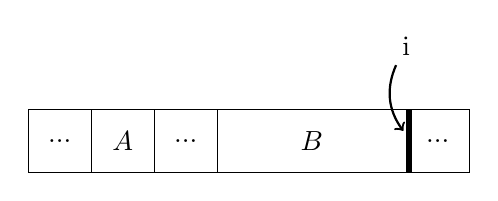
\begin{tikzpicture}[scale=0.8]
      \draw (0, 0) rectangle (1, 1) node [pos=.5] {...}
            (1, 0) rectangle (2, 1) node [pos=.5] {$A$}
            (2, 0) rectangle (3, 1) node [pos=.5] {...}
            (3, 0) rectangle (6, 1) node (rest) [pos=.5] {$B$}
            (6, 0) rectangle (7, 1) node [pos=.5] {...};
      \fill [black] (6, 0) rectangle (6.1, 1) node (ibar) [pos=.5] {};
      \draw (6, 2) node (i) {i};
      \draw[thick, ->] (i) edge [bend right] (ibar);
      \end{tikzpicture}
 \caption{$A$是目前找到的最大子序列和,$B$是以$i$结尾的子序列和。}
 \label{fig:max-sum-invariant}
\end{figure}

\btab{|l|l|r|}
\hline
最大和 & 以$i$结尾的子序列和 & 尚未扫描部分 \\
\hline
0 & 0 & $[3, -13, 19, -12, 1, 9, 18, -16, 15, -15]$ \\
3 & 3 & $[-13, 19, -12, 1, 9, 18, -16, 15, -15]$ \\
3 & 0 & $[19, -12, 1, 9, 18, -16, 15, -15]$ \\
19 & 19 & $[-12, 1, 9, 18, -16, 15, -15]$ \\
19 & 7 & $[1, 9, 18, -16, 15, -15]$ \\
19 & 8 & $[9, 18, -16, 15, -15]$ \\
19 & 17 & $[18, -16, 15, -15]$ \\
35 & 35 & $[-16, 15, -15]$ \\
35 & 19 & $[15, -15]$ \\
35 & 34 & $[-15]$ \\
35 & 19 & $[\ ]$\\
\hline
\etab

\begin{algorithmic}[1]
\Function{Max-Sum}{$V$}
  \State $A \gets 0, B \gets 0, n \gets |V|$
  \For{$i \gets 1$ to  $n$}
    \State $B \gets $ \Call{Max}{$B + V[i], 0$}
    \State $A \gets $ \Call{Max}{$A, B$}
  \EndFor
  \State \Return $A$
\EndFunction
\end{algorithmic}

我们也可以用叠加查找子序列最大和:$S_{max} = fst \circ foldr\ f\ (0, 0)$,其中$f$更新最大和:

\be
f\ x\ (S_m, S) = (S_m' = \max(S_m, S'), S' = \max(0, x + S))
\ee

\begin{Exercise}
\Question{修改最大子序列和的实现,返回对应最大和的子序列。}
\Question{本特利\cite{Bentley}给出了一个分而治之的方法求子数组最大和。复杂度为$O(n \log n)$。思路是将列表在中点分成两份。我们可以递归地找出前半部分的最大和,和后半部分的最大和,和跨越中点部分的最大和。实现这一方法。
}
\Question{在$m \times n$的二维整数矩阵中寻找子矩阵,使得各元素相加后的和最大。}
\end{Exercise}

\begin{Answer}
\Question{修改最大子序列和的实现,返回对应最大和的子序列。

如果除了最大子序列和,还希望返回子序列,我们可以在fold过程中使用两对值$P_m$和$P$,每对值都包括子序列的和与子序列本身$(S, L)$。

\blre
max_s & = & fst \cdot foldr\ f\ ((0, [\ ]), (0, [\ ])) \\
\text{其中}: & & f\ x\ (P_m, (S, L)) = (P_m', P') \\
& & \text{在$f$中}:  P' = max((0, [\ ]), (x + S, x \cons L)), P_m' = max(P_m, P') \\
\elre
}
\Question{本特利\cite{Bentley}给出了一个分而治之的方法求子数组最大和。复杂度为$O(n \log n)$。思路是将列表在中点分成两份。我们可以递归地找出前半部分的最大和,和后半部分的最大和,和跨越中点部分的最大和。实现这一方法。

\begin{algorithmic}[1]
\Function{Max-Sum}{$A$}
  \If{$A = \phi$}
    \State \Return 0
  \ElsIf{$|A| = 1$}
    \State \Return \Call{Max}{$0, A[1]$}
  \Else
    \State $m \gets \lfloor \frac{|A|}{2} \rfloor$
    \State $a \gets$ \textproc{Max-From}(\Call{Reverse}{$A[1...m]$})
    \State $b \gets$ \Call{Max-From}{$A[m+1...|A|]$}
    \State $c \gets$ \Call{Max-Sum}{$A[1...m]$}
    \State $d \gets$ \Call{Max-Sum}{$A[m+1...|A|$}
    \State \Return \textproc{Max}($a+b, c, d$)
  \EndIf
\EndFunction
\Statex
\Function{Max-From}{$A$}
  \State $sum \gets 0, m \gets 0$
  \For{$i \gets 1$ to $|A|$}
    \State $sum \gets sum + A[i]$
    \State $m \gets $ \Call{Max}{$m, sum$}
  \EndFor
  \State \Return $m$
\EndFunction
\end{algorithmic}
复杂度存在递归关系$T(n) = 2T(n/2) + O(n)$。利用主定理可知复杂度为$O(n)$。
}
\end{Answer}

\section{字符串搜索}
字符串搜索是一类实用问题。所有文本编辑软件都带有字符串搜索功能。在基数树、前缀树中(第6章),我们利用特殊的数据结构进行搜索。我们也可以直接在字符串序列中进行搜索,如图\ref{fig:strstr}所示\footnote{编程环境一般会提供一些逐一搜索工具,如C标准库中的\texttt{strstr},C++标准库中的\texttt{find},以及Java标准库中的\texttt{indexOf}。}。

\begin{figure}[htbp]
 \centering
 \subcaptionbox{偏移量$s = 4$,连续$q=4$个字符相同,但第5个字符不同。}{\input{img/strstr.tex}} \\
 \subcaptionbox{偏移到$s = 4 + 2 = 6$。}{\input{img/kmp.tex}}
 \caption{在文本“any ananthous ananym flower”中寻找“ananym”}
 \label{fig:strstr}
\end{figure}

%% \subsection{KMP算法}
\index{KMP} \index{Knuth-Morris-Pratt算法}

在文本$T$中搜索字符串$P$。如图\ref{fig:strstr} (a)所示,在偏移量$s=4$时,逐一检查$P$和$T$中的字符。前4个相等,第5个在$P$中是y,但在$T$中是t。此时逐一比较立即终止,将$s$加1($P$向右移动1个位置)然后重新比较ananym和nantho……我们发现$s$的增量可以超过1。前两个字符an恰好是anan的后缀。我们可以将$s$增加2($P$向右移动2),如图\ref{fig:strstr} (b)所示。我们复用了此前已经比较过4个字符的信息,跳过了无需比较的位置。高德纳、莫里斯、普拉特根据这一想法给出了一个高效的字符串匹配算法\cite{kmp},人们把三人名字的首字母合在一起,称作KMP算法。

记文本$T$中前$k$个字符组成的串为$T_k$($T$的$k$个字符前缀)。为了尽可能多地把$P$向右移动$s$个位置,我们需要利用已成功匹配的$q$个字符。如图\ref{fig:kmp-fallback}所示,若$P$可向右移动,则一定存在某个$k$,使得$P$中的前$k$个字符和前缀$P_q$的最后$k$个字符相同。也就是说,前缀$P_k$同时是$P_q$的后缀。定义空串“”是任何串的前缀和后缀,则总存在最小的$k=0$。我们要找到同时既是前缀又是后缀的最大$k$。定义\textbf{前缀函数}$\pi(q)$,它告诉我们当第$q+1$个字符不匹配时应该回退的位置\cite{CLRS}。

\begin{figure}[htbp]
 \centering
 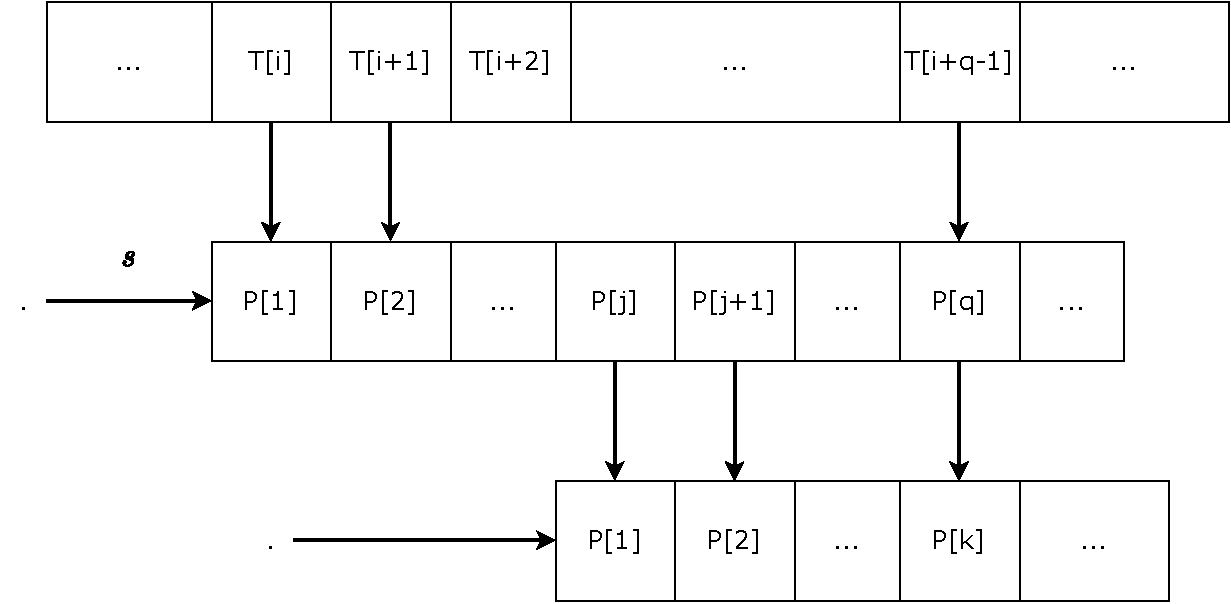
\includegraphics[scale=0.5]{img/kmp-fallback}
 \caption{$P_k$同时是$P_q$的前缀和后缀}
 \label{fig:kmp-fallback}
\end{figure}

\be
\pi(q) = max \{ k | 0 \leq k < q, \text{且} P_k \text{是} P_q \text{的后缀}\}
\label{eq:prefix-function}
\ee

当在文本$T$中偏移$s$匹配$P$时,若前$q$个字符相同,而下一个不同,我们通过$q' = \pi(q)$找到一个回退的位置$q'$。重新比较$P[q']$和文本:

\begin{algorithmic}[1]
\Function{KMP}{$T, P$}
  \State $\pi \gets $ \Call{Build-Prefixes}{$P$}
  \State $n \gets |T|, m \gets |P|, q \gets 0$
  \For{$i \gets 1$ to $n$}
    \While{$q > 0$ 且 $P[q+1] \neq T[i]$}
      \State $q \gets \pi(q)$
    \EndWhile
    \If{$P[q+1] = T[i]$}
      \State $q \gets q + 1$
    \EndIf
    \If{$q = m$}
      \State 位置$i - m$是一个解
      \State $q \gets \pi(q)$ \Comment{寻找更多的匹配位置}
    \EndIf
  \EndFor
\EndFunction
\end{algorithmic}

直接利用式(\ref{eq:prefix-function})构造$\pi(q)$并不实用,我们进一步复用信息,构造前缀函数。如果第一个字符就不匹配,此时最长前缀同时也是后缀的显然是空串:$\pi(1) = 0$。即:$P_k = P_0 = [\ ]$。当扫描到$P$中第$q$个字符时,前缀函数值$\pi(i)$,$i = 1, 2, ..., q-1$都已算好,并且目前最长的前缀$P_k$同时也是$P_{q-1}$的后缀。如图\ref{fig:kmp-prefix-func}所示,若$P[q] = P[k+1]$,则找到了一个更大的$k$,我们将$k$的最大值加一;否则$P[q] \neq P[k + 1]$,我们利用$\pi(k)$回退到一个较短的$P_{k'}$,其中$k' = \pi(k)$,然后比较这个新前缀的下一个字符是否和第$q$个字符相等。重复这一步骤,直到$k$变成0(空串),或者和第$q$个字符相等。下表给出了ananym的前缀函数值,$k$列是满足式(\ref{eq:prefix-function})的最大值。

\begin{figure}[htbp]
 \centering
 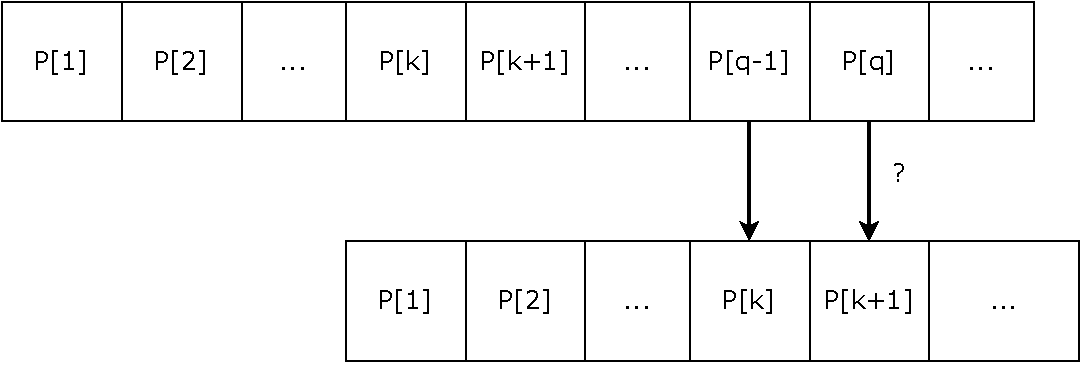
\includegraphics[scale=0.5]{img/kmp-prefix-func}
 \caption{$P_k$是$P_{q-1}$的后缀,比较$P[q]$和$P[k+1]$}
 \label{fig:kmp-prefix-func}
\end{figure}

\btab{|c|r|c|l|}
\hline
$q$ & $P_q$ & $k$ & $P_k$ \\
\hline
1 & a & 0 & ``'' \\
2 & an & 0 & ``'' \\
3 & ana & 1 & a \\
4 & anan & 2 & an  \\
5 & anany & 0 & ``'' \\
6 & ananym & 0 & ``'' \\
\hline
\etab

\begin{algorithmic}[1]
\Function{Build-Prefixes}{$P$}
  \State $m \gets |P|, k \gets 0$
  \State $\pi(1) \gets 0$
  \For{$q \gets 2$ to $m$}
    \While{$k > 0$ 且 $P[q] \neq P[k+1]$}
      \State $k \gets \pi(k)$
    \EndWhile
    \If{$P[q] = P[k+1]$}
      \State $k \gets k + 1$
    \EndIf
    \State $\pi(q) \gets k$
  \EndFor
  \State \Return $\pi$
\EndFunction
\end{algorithmic}

KMP对待搜索串预处理,构建前缀函数的分摊复杂度为$O(m)$\cite{CLRS}。搜索本身的分摊复杂度是$O(n)$。总体分摊复杂度为$O(m + n)$,并需要$O(m)$空间记录前缀函数值。待搜索串的形式并不影响KMP算法的性能。考虑在“aaa...a”($n$个)中搜索长为$m$的子串“aaa...ab”。第$m$个字符不匹配,我们只能回退一个字符,并且此后不断回退1个字符。即使在这种情况下,KMP算法依旧是线性时间的。

% 伯德给出了一个纯函数式的KMP算法(\cite{fp-pearls}第17章)。

%% \subsection{鲍耶-摩尔算法}
%% \index{Boyer-Moore算法}

%% 鲍耶-摩尔在1977年给出了一种字符串匹配算法\cite{boyer-moore}。如图\ref{fig:bad-char}所示,即使按照KMP算法向右平移2仍然匹配失败。待查找字符串ananym长度为6,最后一个字符对应文本中的h。而h根本没有出现在待搜索串中。我们据此可以直接向右平移6。这一规则叫做\textbf{不良字符规则}:对$P$进行预处理。设字符集为$\Sigma$,找到所有不在$P$中的不良字符$B = {c | c \in \Sigma, c \notin P}$。扫描时遇到不良字符就向右移动距离$|P|$。如果不匹配的字符$c \in P$,为了避免漏掉解,我们只能向右移动较短的距离重新搜索,如图\ref{fig:good-char}所示。字符$c$可能在$P$中出现多次,从左向右位于$p_1, p_2, ..., p_i$。为避免遗漏,我们用最后一个位置$p_i$计算平移的距离:

%% \begin{figure}[htbp]
%%  \centering
%%  \includegraphics[scale=0.6]{img/strstr}
%%  \caption{h没有出现在$P$中,应向右侧至少平移6。}
%%  \label{fig:bad-char}
%% \end{figure}

%% \be
%% s = |P| - p_i
%% \label{eqn:BMH-shift}
%% \ee

%% \begin{figure}[htbp]
%%  \centering
%%  \subcaptionbox{e $\neq$ p,但p $\in P$。}{\includegraphics[scale=0.5]{img/good-char}} \\
%%  \subcaptionbox{向右平移2。}{\includegraphics[scale=0.5]{img/good-char-2}}
%%  \caption{不匹配的字符$c \in P$。}
%%  \label{fig:good-char}
%% \end{figure}

%% 我们跳过$c$出现在$P$末尾的情况,此时$p_i = |P|$,平移$s = 0$。由于$s$是相对$P$末尾计算的,从右向左扫描时,一旦匹配失败,我们需要检查待末尾字符$r$在文本中的对应的字符是在不良字符集$B$中,如图\ref{fig:good-char-2}。

%% \begin{figure}[htbp]
%%  \centering
%%  \subcaptionbox{}{\includegraphics[scale=0.5]{img/good-char-3}}
%%  \subcaptionbox{}{\includegraphics[scale=0.5]{img/good-char-4}}
%%  \caption{从右向左检查到i $\neq$ a,用末尾字符e计算平移$s = 6$(e在$P$中出现两次,第二次在末尾,此时$s=0$,需要跳过)。}
%%  \label{fig:good-char-2}
%% \end{figure}

%% 仅使用不良字符规则就可得到简单快速的查找算法,称为鲍耶-摩尔-霍斯普尔算法\cite{boyer-moore-horspool}:

%% \begin{algorithmic}[1]
%% \Procedure{Boyer-Moore-Horspool}{$T, P$}
%%   \State $m \gets |P|, n \gets |T|$
%%   \For{each $c \in \Sigma$}
%%     \State $\pi[c] \gets m$ \Comment{初始化所有平移距离为$m = |P|$}
%%   \EndFor
%%   \For{$i \gets 1$ to $m - 1$} \Comment{跳过末尾位置}
%%     \State $\pi[P[i]] \gets m - i$ \Comment{定义(\ref{eqn:BMH-shift})}
%%   \EndFor
%%   \State $s \gets 0$
%%   \While{$s + m \leq n$}
%%     \State $i \gets m$
%%     \While{$i \geq 1$ 且 $P[i] = T[s+i]$} \Comment{从右向左扫描}
%%       \State $i \gets i - 1$
%%     \EndWhile
%%     \If{$i < 1$}
%%       \State 位置$s$是一个解
%%       \State $s \gets s + 1$ \Comment{寻找下一个解}
%%     \Else
%%       \State $s \gets s + \pi[T[s + m]]$
%%     \EndIf
%%   \EndWhile
%% \EndProcedure
%% \end{algorithmic}

%% 首先将平移表$\pi$的所有值都初始化为$m = |P|$。然后从左向右处理$P$,更新平移距离$\pi(P[i]) = m - i$。如果某个字符出现多次,后面值将覆盖此前的值。将文本和$P$的左侧对齐开始查找。但每个对齐位置$s$,我们都从右向左扫描,如果不匹配就查找$\pi$并移动相应的距离。我们首先用$O(|\Sigma| + |P|)$的时间构造平移表$\pi$。如果字符集不大,复杂度主要由$P$和文本长度决定。最坏情况下,文本和$P$中的字符相同,例如在文本“aa......a”($n$个)中搜索“aa...a”($m$个)。复杂度为$O(mn)$。当$P$较长并且有常数个解时,复杂度为线性时间。

%% 考虑在文本bbbababbabab...中搜索abbabab,如图\ref{fig:bad-char-2}所示。根据不良字符规则,应向右侧平移2。我们可以平移更长的距离。考虑已从右向左成功匹配了6个字符bbabab,由于ab既是$P$的前缀也是已匹配部分的后缀,我们向右平移对齐这个后缀,如图\ref{fig:good-suffix-case1-1}所示。这类似于KMP中的预处理。但并不能总跳过这样多的字符。考虑如图\ref{fig:good-suffix-case2-1}所示的例子,已匹配了bab。虽然前缀ab也是bab的后缀,但却不能平移这么远。因为bab也在其它位置出现过($P$中第3个字符的位置)。为了避免漏掉解,只能向右平移2。

%% \begin{figure}[htbp]
%%  \centering
%%  \subcaptionbox{}{\includegraphics[scale=0.5]{img/bad-char-1}}
%%  \subcaptionbox{}{\includegraphics[scale=0.5]{img/bad-char-2}}
%%  \caption{不良字符规则:向右平移2,对齐字符b。}
%%  \label{fig:bad-char-2}
%% \end{figure}

%% \begin{figure}[htbp]
%%  \centering
%%  \includegraphics[scale=0.5]{img/good-suffix-case1-1}
%%  \caption{由于前缀ab也是已匹配部分的后缀,向右平移对齐ab}
%%  \label{fig:good-suffix-case1-1}
%% \end{figure}

%% \begin{figure}[htbp]
%%  \centering
%%  \subcaptionbox{}{\includegraphics[scale=0.5]{img/good-suffix-case2-1}}
%%  \subcaptionbox{}{\includegraphics[scale=0.5]{img/good-suffix-case2-2}}
%%  \caption{bab也在$P$中其它位置出现(第3~5个字符)。只能向右平移2。}
%%  \label{fig:good-suffix-case2-1}
%% \end{figure}

%% 以上两种情况组成了\textbf{良好后缀规则},如图\ref{fig:good-suffix-cases}所示。下面两种情况之一可向右平移。我们优先使用规则2然后再应用规则1。

%% \begin{enumerate}
%% \item 如果已匹配部分的某个后缀也是$P$的前缀,并且这一后缀不出现在$P$的其它位置,将$P$向右平移对齐这一前缀;
%% \item 如果已匹配部分的某个后缀也出现在$P$的其它位置,将$P$向右侧平移,对齐最右侧出现的位置。
%% \end{enumerate}

%% \begin{figure}[htbp]
%%  \centering
%%  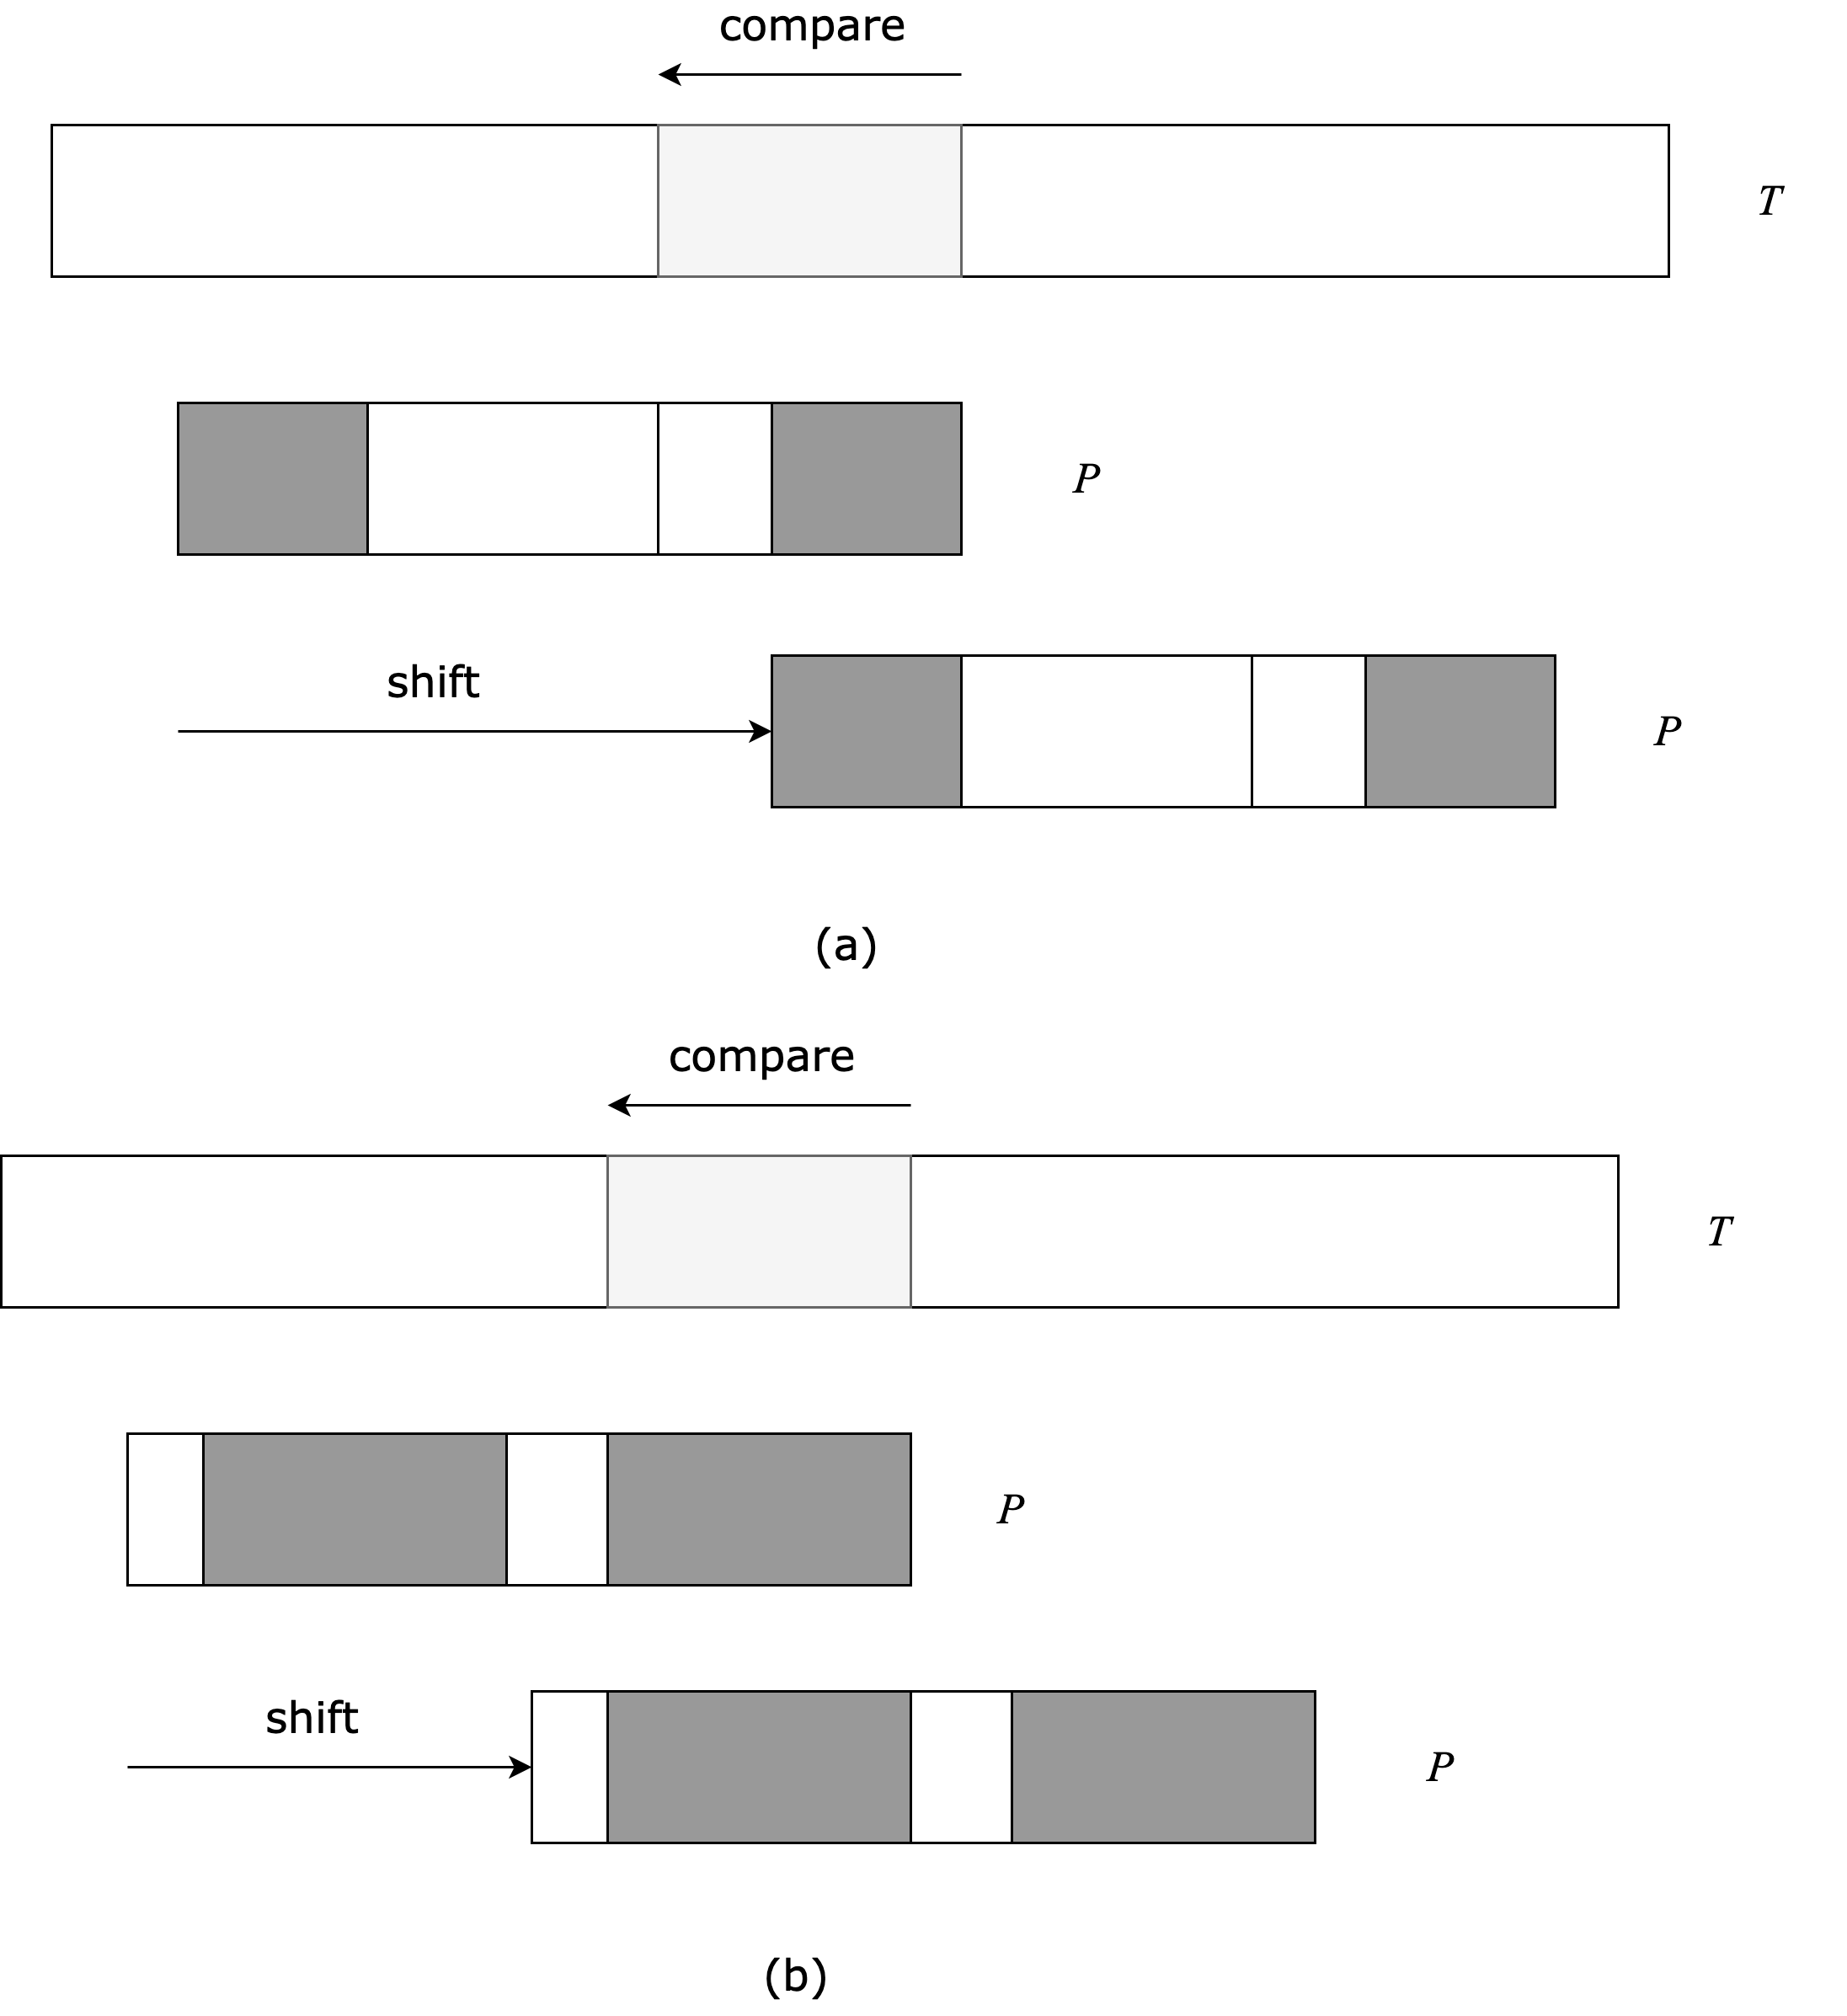
\includegraphics[scale=0.5]{img/BM-good-suffix-rule}
%%  \caption{$T$中浅灰色是已匹配部分,和$P$中深灰色的部分相同。(a) 情况1,已匹配子串中有一部分也是$P$的前缀;(b) 情况2,匹配部分的后缀,也出现在$P$中其它位置。}
%%  \label{fig:good-suffix-cases}
%% \end{figure}

%% 良好后缀规则仅依赖于$P$,可以在搜索前预处理。记$P$中从第$i$个字符开始的后缀为$\overline{P_i} = P[i...m]$,其中$m = |P|$。对规则1,从右向左扫描检查$P$的每个后缀:$\overline{P_m}$, $\overline{P_{m-1}}$, ...,  $\overline{P_2}$是否是$P$的前缀。对规则2,从左向右扫描$P$的每个前缀:$P_1$, $P_2$, ..., $P_{m-1}$,检查它的最长后缀是否也是$P$的后缀:

%% \begin{algorithmic}[1]
%% \Function{Good-Suffix}{$P$}
%%   \State $m \gets |P|$
%%   \State $\pi_s \gets [0, 0, ..., 0]$ \Comment{$m$个}
%%   \State $l \gets 0$                  \Comment{空串}
%%   \For{$i \gets m-1$ down-to $1$}     \Comment{从右向左扫描规则1}
%%     \If{$\overline{P_i} \sqsubset P$} \Comment{$A \sqsubset B$:$A$是$B$的前缀}
%%       \State $l \gets i$
%%     \EndIf
%%     \State $\pi_s[i] \gets l$
%%   \EndFor
%%   \For{$i \gets 1$ to $m$} \Comment{从左向右扫描规则2}
%%     \State $s \gets$ \Call{Suffix-Length}{$P_i$}
%%     \If{$s \neq 0$ 且 $P[i - s] \neq P[m - s]$}
%%       \State $\pi_s[m - s] \gets m - i$
%%     \EndIf
%%   \EndFor
%%   \State \Return $\pi_s$
%% \EndFunction
%% \end{algorithmic}

%% 为了构造良好后缀规则表$\pi_s$,首先从右向左检查$P$的每个后缀$\overline{P_i}$是否是$P$的前缀并记录。然后从左向右检查$P$的每个前缀,调用函数\textproc{Suffix-Length}($P_i$)找出同时是$P$前缀的后缀的最长长度$s$,若$s \neq 0$,则修改表格$\pi_s$中倒数第$s$项的值。为避免重复找到已匹配的后缀,需要检查$P[i - s]$和$P[m - s]$是否相等。\textproc{Suffix-Length}的实现如下:

%% \begin{algorithmic}[1]
%% \Function{Suffix-Length}{$P_i$}
%%   \State $m \gets |P|, j \gets 0$
%%   \While{$P[m - j] = P[i - j]$ 且 $j < i$}
%%     \State $j \gets j + 1$
%%   \EndWhile
%%   \State \Return $j$
%% \EndFunction
%% \end{algorithmic}

%% 可以同时应用不良字符规则和良好后缀规则,比较并选择较大的平移值:

%% \begin{algorithmic}[1]
%% \Function{Boyer-Moore}{$T, P$}
%%   \State $n \gets |T|, m \gets |P|$
%%   \State $\pi_b \gets$ \Call{Bad-Character}{$P$}
%%   \State $\pi_s \gets$ \Call{Good-Suffix}{$P$}
%%   \State $s \gets 0$
%%   \While{$s + m \leq n$}
%%     \State $i \gets m$
%%     \While{$i \geq 1$ 且 $P[i] = T[s + i]$}
%%       \State $i \gets i - 1$
%%     \EndWhile
%%     \If{$i < 1$}
%%       \State 位置$s$是一个解
%%       \State $s \gets s + 1$ \Comment{继续寻找下一个解}
%%     \Else
%%       \State $s \gets s + max(\pi_b[T[s + m]], \pi_s[i])$
%%     \EndIf
%%   \EndWhile
%% \EndFunction
%% \end{algorithmic}

%% 在最坏的情况下,只有当$P$不出现在文本中时复杂度才是$O(n+m)$\cite{boyer-moore}。如果$P$出现,则复杂度为$O(nm)$。伯德给出了算法的一种纯函数式实现(\cite{fp-pearls}第16章)。

\section{解的搜索}

在早期人工智能阶段,人们发展出了许多方法搜索解。不同于字符串匹配,解并不一定直接存在于一个候选答案集中。往往需要一边构造解一边尝试。某些问题可解,某些问题无解。也可能存在多个解。例如存在多条走出迷宫的路线。人们还需要求出某种意义下的最优解。

\subsection{深度优先和广度优先搜索}
\index{DFS} \index{深度优先搜索}
深度优先搜索(DFS)和广度优先搜索(BFS)常被叫做“图搜索”算法。我们简单介绍这两种搜索算法而略过图的概念。

\subsubsection{迷宫}
\index{迷宫问题}
走迷宫是一类历史悠久的趣题。有窍门说:当遇到分叉时总向右转。这个方法有缺陷,如图\ref{fig:maze-loop}所示,不断向右会绕着中心的大方块转圈。存在多个选项时,决策直接影响到最终的解。童话故事提供了一种思路:携带一块面包进入迷宫。遇到岔路时任选一条道路,并留下一小块面包屑记录下这次尝试。遇到了死胡同就沿着留下的面包屑向回走到上次做出选择的地方,然后换一条路。一旦发现地上已经有面包屑了,就说明我们进入了循环,必须回退并重新尝试。不断这样的“尝试——检查”,我们要么最终走出迷宫,要么退回起点(无解)。我们用用$m \times n$的矩阵$M$描述迷宫,元素值为0、1,表示是否有路。图\ref{fig:maze-loop}的迷宫可以用下面的矩阵定义:

\begin{figure}[htbp]
 \centering
 \subcaptionbox{迷宫}{\includegraphics[scale=0.3]{img/maze}}
 \subcaptionbox{一直右转陷入循环}{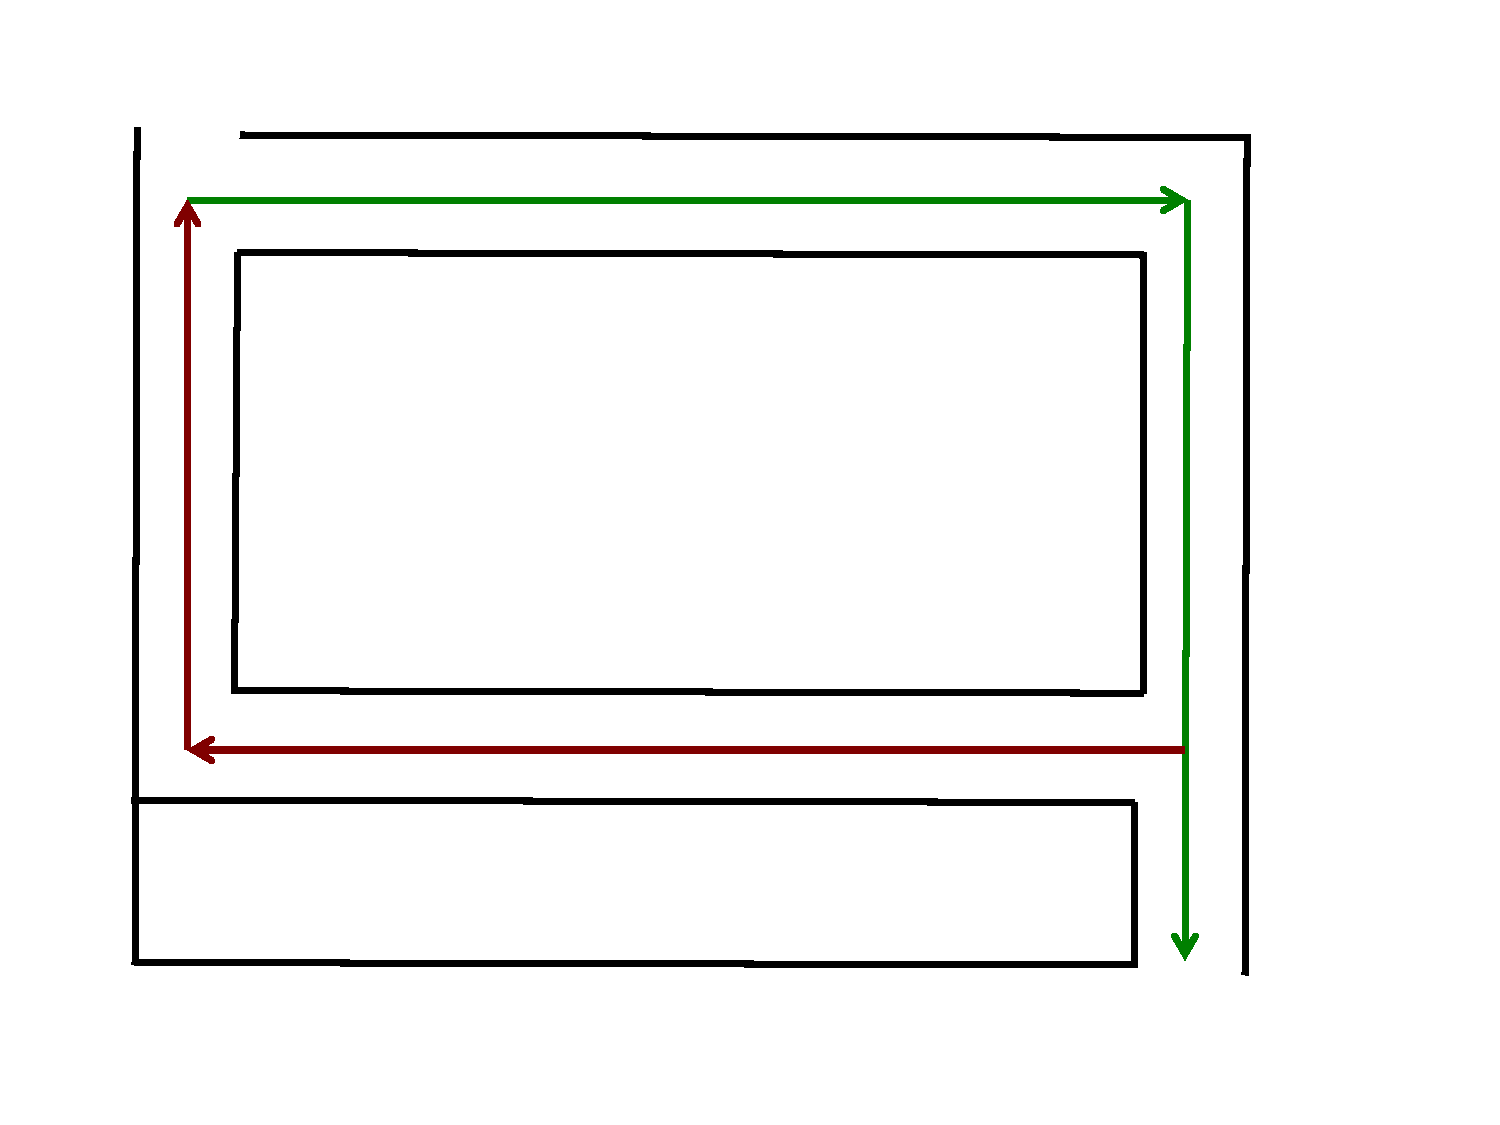
\includegraphics[scale=0.6]{img/maze-loop}}
 \caption{迷宫}
 \label{fig:maze-loop}
\end{figure}

\[
M = \begin{matrix}
0 & 0 & 0 & 0 & 0 & 0 \\
0 & 1 & 1 & 1 & 1 & 0 \\
0 & 1 & 1 & 1 & 1 & 0 \\
0 & 1 & 1 & 1 & 1 & 0 \\
0 & 1 & 1 & 1 & 1 & 0 \\
0 & 0 & 0 & 0 & 0 & 0 \\
1 & 1 & 1 & 1 & 1 & 0
\end{matrix}
\]

给定起点$s=(i, j)$、终点$e=(p, q)$,我们要找出所有从$s$到$e$的通路。我们先找出所有和$s$连通的相邻点,对每个邻点$k$,递归找出从$k$到$e$所有路径。然后将通路$s$-$k$连接到每个从$k$到$e$的路径前。我们需要留下一些“面包屑”标记以避免重复。我们用一个列表$P$记录走过的所有位置。每次检查此列表,只尝试新路径。

\be
\textit{solveMaze}\ M\ s\ e = \textit{solve}\ s\ [[\ ]]
\label{eq:solve-maze-reversed}
\ee

其中:

\be
\textit{solve}\ s\ P = \begin{cases}
  s = e: & map\ (\textit{reverse} \circ (s:))\ P \\
  \text{否则}: & \textit{concat}\ [\textit{solve}\ k\ (map\ (s:)\ P) | k \gets adj\ s, k \notin P] \\
  \end{cases}
\ee

$P$中保存的路径是逆序的,我们需要最终通过\textit{reverse}将其反转。$adj\ p$找出$p$相连通的邻点:水平、垂直方向上相邻为0的点:

\be
\begin{array}{ll}
adj\ (x, y) = [(x', y') | & (x', y') \gets [(x-1, y), (x+1, y), (x, y-1), (x, y+1)], \\
 & 1 \leq x' \leq m, 1 \leq y' \leq n, M_{x' y'} = 0\} \\
\end{array}
\ee

这是一种穷举解法,搜索所有路径。为了走出迷宫,只需要找到一条路径。我们需要某种数据结构保存“面包屑”,记录此前做出的决策。我们总在最新决策基础上搜索通路,这是后进先出的顺序。可以用一个栈来实现。开始时,栈中只有起点$[s]$。将其弹出,找出和$s$连通的点,例如$a$、$b$……将可能的路径$[a, s]$、$[b, s]$入栈。接下来将路径$[a, s]$弹出,检查和$a$连通的点。然后把所有3步可达的路径入栈。重复这一过程。栈中记录了一条条逆序路径:从起点开始通向可达的最远位置,如图\ref{fig:dfs-stack}所示。当栈变为空时,我们已尝试了所有的可能,仍未找到通路,迷宫无解;否则弹出栈顶的候选路径,扩展未曾走过的连通邻点,然后入栈。

\begin{figure}[htbp]
 \centering
 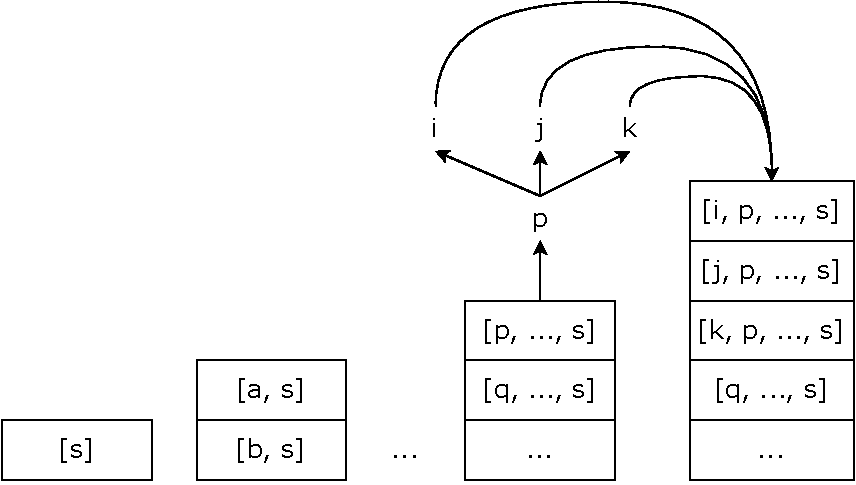
\includegraphics[scale=0.5]{img/dfs-stack}
 \caption{用栈记录路径}
 \label{fig:dfs-stack}
\end{figure}

\be
\textit{solveMaze}\ M\ s\ e = \textit{solve}\ [[s]]
\ee

其中:

\be
\begin{array}{rcl}
\textit{solve}\ [\ ] & = & [\ ] \\
\textit{solve}\ ((p \cons ps) \cons cs) & = & \begin{cases}
  c = e: & \textit{reverse}\ (p \cons ps) \\
  ks = [\ ]: & \textit{solve}\ cs, \text{其中}\ ks = filter\ (\notin ps)\ (adj\ p) \\
  ks \neq [\ ]: & \textit{solve}\ ((map\ (:p \cons ps)\ ks) \doubleplus cs)
  \end{cases}
\end{array}
\ee

对应的迭代实现如下:

\begin{algorithmic}[1]
\Function{Solve-Maze}{$M, s, e$}
  \State $S \gets [s], L = [\ ]$
  \While{$S \neq [\ ]$}
    \State $P \gets$ \Call{Pop}{$S$}
    \State $p \gets$ \Call{Last}{$P$}
    \If{$e = p$ }
      \State \Call{Add}{$L, P$}   \Comment{找到一个解}
    \Else
      \For{each $k$ in \Call{Adjacent}{$M, p$}}
        \If{$k \notin P$}
          \State \Call{Push}{$S, P \doubleplus [k]$}
        \EndIf
      \EndFor
    \EndIf
  \EndWhile
  \State \Return $L$
\EndFunction
\end{algorithmic}

每步有上下左右4个选项可能入栈,并且都在回溯时检查。复杂度看似是$O(4^n)$,其中$n$是路径长度。实际复杂度不会这样大,我们跳过了已走的位置。最坏情况下,所有可达点都恰好被访问过一次,复杂度为$O(n)$,其中$n$是连通点的数量。由于使用了栈来保存路径,空间复杂度为$O(n^2)$。

\subsubsection{八皇后问题}
\index{八皇后问题}

虽然国际象棋历史悠久,但直到1848年贝策尔(Max Bezzel)才提出八皇后趣题\cite{wiki-8-queens}。皇后威力巨大,可以攻击同一行、列、斜线上的任意棋子。如何在棋盘上摆下八个皇后,而她们之间不互相攻击。图\ref{fig:8-queens-puzzle} (a)描述了皇后可以攻击到的范围。图\ref{fig:8-queens-puzzle} (b)给出了八皇后问题的某一种解。

\begin{figure}[htbp]
 \centering
 \subcaptionbox{国际象棋中的皇后}{\includegraphics[scale=1]{img/queen}}
 \subcaptionbox{一种解}{\includegraphics[scale=1]{img/queens-example}}
 \caption{八皇后问题}
 \label{fig:8-queens-puzzle}
\end{figure}

在64个格子中放入8个皇后,共有$P^8_{64}$种排列,约为$4 \times 10^{10}$。每行、列只能摆放1个皇后,一个解的布局必然是$[1,2,3,4,5,6,7,8]$的某种排列。例如布局$[6,2,7,1,3,5,8,4]$表示第一行的皇后放在第6列;第二行的皇后摆在第2列上……第8行的皇后摆在第4列。这样我们只需要检查$8! = 40320$种布局。从第一行开始逐一摆放皇后。第一个皇后有8种摆法(八列中的某一列)。摆放第二行的皇后时,由于可能和第一个皇后相互攻击,需要避开某些列。对于第$i$行的皇后,找到8列中不被前$i-1$个皇后攻击的位置。如果8个位置都不能摆放,我们就回退调整以前$i-1$个皇后。全部8个皇后都成功放入棋盘后,就找到了一个解。为了找出所有解,我们记录下这一布局,然后继续检查其它可能的列并进行必要的回溯。我们用一个栈和一个列表启动搜索:$solve\ [[\ ]]\ [\ ]$

\be
\begin{array}{rcl}
solve\ [\ ]\ s & = & s \\
solve\ (c \cons cs)\ s & = & \begin{cases}
  |c| = 8: & solve\ cs\ (c \cons s) \\
  \text{否则}: & solve\ ( [ x \cons c | x \gets [1..8], x \notin c, \textit{safe}\ x\ c] \doubleplus cs)\ s
  \end{cases}
\end{array}
\ee

若栈为空,我们已经尝试所有可能,$s$记录了所有找到的解;若栈顶布局$c$长度为8,我们找到了一个解。将其记录到$s$中,然后继续查找;若$|c| < 8$,我们从8列中找出尚未被占的列($x \notin c$),同时不能被斜线上的其它皇后攻击(通过\textit{safe} $x c$)。可行的布局入栈用于此后的搜索。

\be
\textit{safe}\ x\ c = \forall (i, j) \gets zip\ \textit{reverse}\ c, [1, 2, ...] \text{有} |x - i| \neq |y - j|, \text{其中} y = 1 + |c|
\ee

\textit{safe}检查如果第$y = 1 + |c|$行,$x$列的皇后是否和$c$中任何皇后成对角线。若$c = [i_{y-1}, i_{y-2}, ..., i_1]$是前$y-1$个皇后所在的列,我们将$c$反转,并和1, 2, ...组成每个皇后的坐标:$[(i_1, 1), (i_2, 2), ..., (i_{y-1}, y-1)\}$。然后判断每个$(i, j)$是否和位置$(x, y)$构成对角线:$|x - i| \neq |y - j|$。

这一实现是尾递归的,可以消除递归优化为迭代实现:

\begin{algorithmic}[1]
\Function{Solve-Queens}{}
  \State $S \gets [[\ ]]$
  \State $L \gets [\ ]$ \Comment{保存解}
  \While{$S \neq [\ ]$}
    \State $A \gets$ \Call{Pop}{$S$} \Comment{$A$是某一中间布局}
    \If{$|A|=8$}
      \State \Call{Add}{$L, A$}
    \Else
      \For{$i \gets 1$ to $8$}
        \If{\Call{Valid}{$i, A$}}
          \State \Call{Push}{$S, A \doubleplus [i]$}
        \EndIf
      \EndFor
    \EndIf
  \EndWhile
  \State \Return $L$
\EndFunction
\Statex
\Function{Valid}{$x, A$}
  \State $y \gets 1 + |A|$
  \For{$i \gets 1$ to $|A|$}
    \If{$x = A[i]$ 或 $|y-i| = |x - A[i]|$}
      \State \Return False
    \EndIf
  \EndFor
  \State \Return True
\EndFunction
\end{algorithmic}

虽然每个皇后有8列选择,但只尝试尚未被占的列。总共检查15720种情况,远远小于$8^8 = 16777216$种可能\cite{wiki-8-queens}。由于正方形棋盘水平、垂直都对称,找到一个解后,通过旋转、翻转可以得到其它对称解。我们可以扩展到$n$皇后问题,其中$n \geq 4$。但随着$n$增大所用时间急速增加。回溯算法仅比枚举8的全排列稍快(枚举全排列的时间是$O(n!)$)。

\subsubsection{跳棋趣题}
\index{跳棋趣题}

如图\ref{fig:leapfrog},在一排7块石头上有6只青蛙。一块石头只够一只青蛙停在上面。青蛙可以跳到它前方的石头上,或越过一只青蛙跳到更前方的石头上。青蛙只能前进或停止,不能后退,如图\ref{fig:pegrules}。这些青蛙如何移动、跳跃,使得左右3只位置互换?标记左侧青蛙为-1,右侧为1,没有青蛙的石头为0,我们要找到从$s = [-1, -1, -1, 0, 1, 1, 1]$转换到$e = [1, 1, 1, 0, -1, -1, -1]$的解。

\begin{figure}[htbp]
 \centering
 \includegraphics[scale=0.4]{img/leapfrogs}
 \caption{跳跃的青蛙}
 \label{fig:leapfrog}
\end{figure}

\begin{figure}[htbp]
 \centering
 \subcaptionbox{跳到相邻的石头上}{\includegraphics[scale=0.3]{img/leapfrog1}} \hspace{0.02\textwidth}
 \subcaptionbox{向右越过一只}{\includegraphics[scale=0.3]{img/leapfrog2}} \hspace{0.02\textwidth}
 \subcaptionbox{向左越过一只}{\includegraphics[scale=0.3]{img/leapfrog3}}
 \caption{移动规则}
 \label{fig:pegrules}
\end{figure}

这是跳棋的一种特殊形式。并不一定限制为6颗棋子,也可以是8或者更大的偶数。图\ref{fig:pegpuzzles}是这类问题的变化形式\footnote{图片来源:\url{http://www.robspuzzlepage.com/jumping.htm}}。

\begin{figure}[htbp]
 \centering
 \subcaptionbox{}{\includegraphics[scale=0.5]{img/solitaire}} \hspace{0.02\textwidth}
 \subcaptionbox{}{\includegraphics[scale=0.7]{img/hop-over}} \hspace{0.02\textwidth}
 \subcaptionbox{}{\includegraphics[scale=0.3]{img/draught-board}}
 \caption{三种跳棋趣题}
 \label{fig:pegpuzzles}
\end{figure}

从左向右的石头位置为1, 2, ..., 7。每次有4种移动可能。例如开始时,第3块石头上的青蛙可以移动到空石头上。对称地,第5块石头上的青蛙也可以左移一步。第2块石头上的青蛙可以向右越过一只青蛙跳到空石头上,对称地,第6块石头上的青蛙,也可以向左越过一只。每次记录下7块石头和青蛙的状态,尝试4种方案。如果走不下去了,就回溯尝试其它方案。由于左侧的青蛙只能向右,右侧的只能向左,所有移动都是不可逆的。和走迷宫不同,这里不存在重复情况。我们记录移动的步骤用于最后输出结果。状态$L$是$s$的某种排列。$L[i]$的值是$\pm 1, 0$表示第$i$个石头是空的、有一只向左、向右的青蛙。令空石头的位置为$p$,4种移动方案为:

\begin{enumerate}
\item 向左跳跃:$p < 6$,且$L[p+2] > 0$,交换$L[p] \leftrightarrow L[p+2]$;
\item 向左移动:$p < 7$,且$L[p+1] > 0$,交换$L[p] \leftrightarrow L[p+1]$;
\item 向右跳跃:$p > 2$,且$L[p-2] < 0$,交换$L[p-2] \leftrightarrow L[p]$;
\item 向右移动:$p > 1$,且$L[p-1] < 0$,交换$L[p-1] \leftrightarrow L[p]$。
\end{enumerate}

定义4个函数$leap_l$、$hop_l$、$leap_r$、和$hop_r$,变化状态$L \mapsto L'$。若不能移动,则返回同样的$L$不变。使用栈$S$记录已做过的尝试。开始的时候,栈中只有一个列表,列表中只有开始状态。列表$M$记录所有找到的解。我们不断取出栈顶。如果状态$L = e$则找到了一个解。我们将移动步骤记录到$M$中。否则我们在$L$上尝试4种移动,如果可行就入栈以备继续搜索。

\be
solve\ [[-1, -1, -1, 0, 1, 1, 1]]\ [\ ]
\ee

其中:

\be
\begin{array}{rcl}
solve\ [\ ]\ s & = & s \\
solve\ (c \cons cs)\ s & = & \begin{cases}
  L = e: & solve\ cs (\textit{reverse}\ c : s), \text{其中} L = head\ c\\
  \text{否则}: & solve\ ((map\ (:c)\ (moves\ L)) \doubleplus cs)\ s \\
  \end{cases}
\end{array}
\ee

$moves$在状态$L$之上尝试4中可能的移动:

\be
moves\ L = filter (\neq L)\ [leap_l\ L, hop_l\ L, leap_r\ L, hop_r\ L]
\ee

对应的迭代实现如下:

\begin{algorithmic}[1]
\Function{Solve}{$s, e$}
  \State $S \gets [[s]]$
  \State $M \gets [\ ]$
  \While{$S \neq [\ ]$}
    \State $s \gets$ \Call{Pop}{$S$}
    \If{$s[1] = e$}
      \State \textproc{Add}($M$, \Call{Reverse}{$s$})
    \Else
      \For{each $m$ in \Call{Moves}{$s[1]$}}
        \State \textproc{Push}($S$, $m \cons s$)
      \EndFor
    \EndIf
  \EndWhile
  \State \Return $M$
\EndFunction
\end{algorithmic}

这一方法找出两个左右对称解(各15步),下表列出了一个:

\btab{|c||c|c|c|c|c|c|c|}
\hline
步骤 & -1 & -1 & -1 & 0 & 1 & 1 & 1 \\
\hline
1 & -1 & -1 & 0 & -1 & 1 & 1 & 1 \\
2 & -1 & -1 & 1 & -1 & 0 & 1 & 1 \\
3 & -1 & -1 & 1 & -1 & 1 & 0 & 1 \\
4 & -1 & -1 & 1 & 0 & 1 & -1 & 1 \\
5 & -1 & 0 & 1 & -1 & 1 & -1 & 1 \\
6 & 0 & -1 & 1 & -1 & 1 & -1 & 1 \\
7 & 1 & -1 & 0 & -1 & 1 & -1 & 1 \\
8 & 1 & -1 & 1 & -1 & 0 & -1 & 1 \\
9 & 1 & -1 & 1 & -1 & 1 & -1 & 0 \\
10 & 1 & -1 & 1 & -1 & 1 & 0 & -1 \\
11 & 1 & -1 & 1 & 0 & 1 & -1 & -1 \\
12 & 1 & 0 & 1 & -1 & 1 & -1 & -1 \\
13 & 1 & 1 & 0 & -1 & 1 & -1 & -1 \\
14 & 1 & 1 & 1 & -1 & 0 & -1 & -1 \\
15 & 1 & 1 & 1 & 0 & -1 & -1 & -1 \\
\hline
\etab

每侧有3只青蛙时需要15步左右互换。扩展上述解法可以得到步数和青蛙数目的一个关系表:

\btab{c|c|c|c|c|c|c}
每侧青蛙数$n$ & 1 & 2 & 3  & 4  & 5 & ... \\
\hline
解法步数 & 3 & 8 & 15 & 24 & 35 & ...
\etab

步数恰好是完全平方数减一:$(n+1)^2 - 1$。我们可以证明这一结论:
\begin{proof}
比较最终和起始状态,每只青蛙都向另一侧移动了$n+1$块石头。$2n$只青蛙总共移动了$2n(n+1)$块石头。左侧的每只青蛙必然和右侧的所有青蛙相遇一次。一旦相遇,必然发生跳跃。由于一共有$n^2$次相遇,因此共导致了所有青蛙前进了$2n^2$块石头。剩下的移动不是跳跃,而是跳到相邻的石头上,总共有$2n(n+1) - 2n^2 = 2n$次。将$n^2$次跳跃,和$2n$次跳到相邻石头上相加。得到最终解的步数为:$n^2 + 2n = (n+1)^2 -1$。
\end{proof}

观察上面3个趣题,它们的解法有着类似的结构。它们都从某种状态开始。走迷宫从入口开始,八皇后问题从空棋盘开始,跳跃青蛙问题从[-1, -1, -1, 0, 1, 1, 1]开始。解的过程是一种搜索。每次尝试都有若干种可能的选项。走迷宫时,每步有上下左右四个方向选择;八皇后问题中,每次摆放都有八列选择;跳跃青蛙趣题中,每次有4种不同的跳跃方式选择。虽然每次选择都不知道能继续走多远。但我们始终清楚地知道最终状态是什么。走迷宫的最终状态是出口;八皇后问题的最终状态是八个皇后都摆在棋盘上;跳跃青蛙趣题的最终状态是左右青蛙位置互换。

我们使用相同的策略来解决这些问题:不断尝试可能的选项,记录已经达到的状态,如果无法继续就回溯并尝试其它选项。通过这样的方法,我们或者找到解,或者穷尽所有可能而发现问题无解。当然,这类解法存在一些变化,当找到一个解后,我们可以停下结束或者继续寻找所有可能的解。如果以起始状态为根,画出一棵树,每个树枝代表不同的选择。搜索过程是一个不断深入的过程。只要能继续,我们先不考虑同一深度上的其它选项。直到失败后回溯到树的上一层。如图\ref{fig:dfs-tree}中的搜索顺序。箭头描述了如何先向下,在向上回溯的过程。节点上的数字是访问顺序。

\begin{figure}[htbp]
 \centering
 \includegraphics[scale=0.6]{img/dfs-tree}
 \caption{深度优先搜索的顺序}
 \label{fig:dfs-tree}
\end{figure}

这样的搜索策略称为深度优先搜索。现实中我们在不经意间广泛使用它。某些编程环境,例如Prolog,使用深度优先作为默认的求值模型。例如一个迷宫可以被一组规则描述:

\lstset{language=Prolog}
\begin{lstlisting}
c(a, b). c(a, e).
c(b, c). c(b, f).
c(e, d), c(e, f).
c(f, c).
c(g, d). c(g, h).
c(h, f).
\end{lstlisting}

其中,断言$c(X, Y)$表示位置$X$和$Y$连通。这一断言是有方向性的。如果要让$Y$和$X$连通,我们可以增加一条对称的断言,或者建立一条无方向性的断言。图\ref{fig:directed-graph}给出了一个有向图。任给位置$X$和$Y$,Prolog可以通过下面的程序判定它们之间是否有通路。

\begin{figure}[htbp]
 \centering
 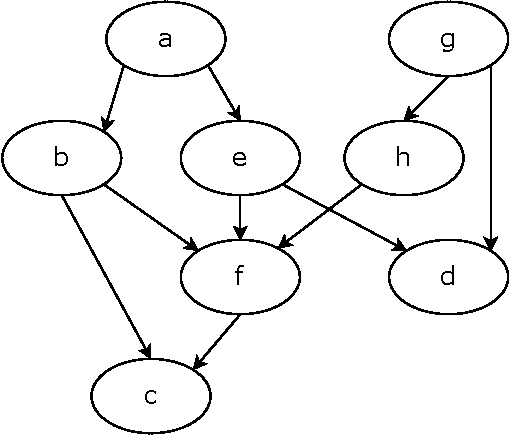
\includegraphics[scale=0.5]{img/directed-graph}
 \caption{一个有向图}
 \label{fig:directed-graph}
\end{figure}

\lstset{language=Prolog}
\begin{lstlisting}
go(X, X).
go(X, Y) :- c(X, Z), go(Z, Y)
\end{lstlisting}

这一程序说:一个位置$X$和自己相通。任意两个不同位置$X$、$Y$,若$X$和$Z$相连,且$Z$和$Y$之间有通路,则$X$和$Y$之间存在通路。显然,$Z$的选择可能不唯一。Prolog选择一个,然后继续搜索。只有当递归搜索失败时才会尝试其它选择。回溯并更换到下一个选项上。这恰好就是深度优先的搜索策略。当只需要找到解,而并不关心步数时,深度优先搜索是很有效的方法。例如,走迷宫中找出的第一个解并不一定是最短路径。

\subsubsection{狼、羊、白菜过河问题}
\index{狼、羊、白菜趣题}

这是一道传统趣题。农夫带着一只狼、一只羊、一筐白菜过河。有一条小船,只有农夫会划船。小船只能装下农夫和另外一样东西。农夫每次只能在狼、羊、白菜中任选一样和他一起过河。但是如果农夫不在,狼会吃掉羊,而羊会吃掉白菜。如何用最快的方法让所有东西都渡过河?

%% \begin{figure}[htbp]
%%  \centering
%%  \includegraphics[scale=0.3]{img/wgc-puzzle}
%%  \caption{狼、羊、白菜过河问题}
%%  \label{fig:wgc-puzzle}
%% \end{figure}

由于狼不会吃掉白菜,农夫可以安全地将羊运到河对岸并返回。接下来无论将狼或白菜中的任何一样运过河,他必须将某一样运回以避免有东西被吃掉。为了寻找最快的渡河方法,我们并发检查所有的选项,比较哪个更快。不考虑渡河的方向,每渡过一次算做一步,往返算两步。我们检查渡河一次后的所有可能、两次后所有可能、三次后的所有可能……直到某次后,所有的东西都到达了对岸结束。并且这一渡河方法在所有可能中胜出,是最快的解法。

如何“并发”检查所有可能的解法?考虑一个抽奖游戏。参与者闭着眼睛从箱子里摸出一个球。箱子里只有一个黑球,其余的球都是白色的。摸到黑球获胜,摸到白球则放回箱子,然后等待下次摸球。为了使游戏公平,可以制定这样一个规则:必须等所有人都摸过之后才能再摸第二次。参与游戏的人站成一队。每次站在队伍前面的人摸球,如果他没有摸到黑球获胜,就站到队尾等待下次摸球。这一队列可以保证游戏的公平。

\begin{figure}[htbp]
 \centering
 \includegraphics[scale=1]{img/lucky-draw}
 \caption{第$i$个人出队摸球。如果没有摸到黑球就站到队尾}
 \label{fig:luck-draw}
\end{figure}

用类似的思路来解决渡河问题。用集合$A$、$B$代表河两岸。开始时,集合$A = \{w, g, c, p\}$包含狼、羊、白菜、农夫,集合$B = \nil$。每次将农夫和另外一个元素在集合见移动。如果集合中不存在农夫,则不能含相互冲突的东西。目标是用最少的次数交换$A$、$B$的内容。使用一个队列$Q$包含起始状态$A = \{w, g, c, p\}$、$B=\nil$。只要队列不空,我们就取出头部元素,扩展所有可能的选择。然后将扩展后的状态放回队尾。如果队列头部等于$A=\nil$、$B=\{w, g, c, p\}$,我们就找到了解。图\ref{fig:bfs-tree}描述了搜索顺序。同一深度上的所有可能都被检查了,无需进行回溯。

\begin{figure}[htbp]
 \centering
 \includegraphics[scale=0.5]{img/bfs-tree}
 \caption{从第一个状态开始,检查第二步的所有选项2、3、4;然后检查第3层上的所有选项……}
 \label{fig:bfs-tree}
\end{figure}

可以用4位二进制数来表示集合,每一位表示一种事物,狼$w=1$、羊$g=2$、白菜$c=4$、农夫$p=8$。0表示空集,15表示包含所有事物的集合。值3表示只有狼和羊,此时狼会吃掉羊。同样,值6表示另一种冲突情况。每次我们将最高位(8)和另外一位(4、2、1)从一个数字移动到另一个数字上。可行的移动方法为:

\be
mv\ A\ B = \begin{cases}
  B < 8: & [(A - 8 - i, B + 8 + i) | i \gets [0, 1, 2, 4], i = 0 \text{或} A \overline{\land} i \neq 0]\\
  \text{否则}: & [(A + 8 + i, B - 8 - i) | i \gets [0, 1, 2, 4], i = 0 \text{或} B \overline{\land} i \neq 0]
  \end{cases}
\ee

其中$\overline{\land}$表示按位与运算。我们用队列$Q = \{[(15, 0)]\}$启动搜索:$solve\ Q$。

\be
\begin{array}{rcl}
solve\ \nil & = & \nil \\
solve\ Q & = & \begin{cases}
  A = 0: & reverse\ c, \text{其中} (A, B) = c, (c, Q') = pop\ Q \\
  \text{否则}: & solve\ (pushAll\ (map\ (:c)\ (filter\ (valid\ c)\ (mv\ A\ B)))\ Q')
  \end{cases}
\end{array}
\ee

其中函数$valid\ c$检查新的移动结果$(A, B)$是存在冲突。不能是3、6,并且尚未尝试过,不存在于$c$中:

\be
valid\ c\ (A, B) = A, B \neq 3 \text{或} 6, (A, B) \notin c
\ee

下面是对应的迭代实现:

\begin{algorithmic}[1]
\Function{Solve}{}
  \State $S \gets []$
  \State $Q \gets \{[(15, 0)]\}$
  \While{$Q \neq \nil$}
    \State $C \gets $ \Call{DeQ}{$Q$}
    \If{$C[1] = (0, 15)$}
      \State \textproc{Add}($S$, \Call{Reverse}{$C$})
    \Else
      \For{each $m$ in \Call{Moves}{$C$}}
        \If{\Call{Valid}{$m, C$}}
          \State \Call{EnQ}{$Q, m \cons C$}
        \EndIf
      \EndFor
    \EndIf
  \EndWhile
  \State \Return $S$
\EndFunction
\end{algorithmic}

下面列出了两个最优解。

\btab{l|c|l}
左 & 河 & 右 \\
\hline
狼、羊、白菜、农夫 &   & \\
狼、白菜 &   & 羊、农夫 \\
狼、白菜、农夫 &   & 羊 \\
白菜 &   & 狼、羊、农夫 \\
羊、百次、农夫 &   & 狼 \\
羊 &   & 狼、白菜、农夫 \\
羊、农夫 &   & 狼、白菜 \\
 &  & 狼、羊、白菜、农夫
\etab

\btab{l|c|l}
左 & 河 & 右 \\
\hline
狼、羊、白菜、农夫 & & \\
狼、白菜 & & 羊、农夫 \\
狼、白菜、农夫 & & 羊 \\
狼 & & 羊、白菜、农夫 \\
狼、羊、农夫 & & 白菜 \\
羊 & & 狼、白菜、农夫 \\
羊、农夫 & & 狼、白菜 \\
 & & 狼、羊、白菜、农夫
\etab

\subsubsection{倒水问题}
\index{倒水问题}

有两个水瓶,一个9升、一个4升。如何才能从河中取出6升水?这个题目可以追溯到古希腊。有一个故事说法国数学家泊松在孩童时代就解决了这个问题。在好莱坞电影《虎胆龙威3》中也出现了这个问题。数学家波利亚在《如何解题》中用倒推法给出了一个解\cite{how-to-solve-it}。最终状态大瓶子中盛有6升水。倒数第二步时,从9升的瓶子中倒出3升水。为了达成这一点,小瓶子中需要盛有1升水。如图\ref{fig:jugs-r1}所示。

%% \begin{figure}[htbp]
%%  \centering
%%  \includegraphics[scale=0.5]{img/jugs-start}
%%  \caption{9升、4升的瓶子}
%%  \label{fig:jugs-start}
%% \end{figure}

\begin{figure}[htbp]
 \centering
 \includegraphics[scale=0.5]{img/jugs-r1}
 \caption{最后两步}
 \label{fig:jugs-r1}
\end{figure}

只要倒满9升的瓶子,然后连续两次倒入4升的瓶子,并将4升的瓶子倒空,就可以得到1升水。如图\ref{fig:jugs-r2}所示。倒推法是一种策略,而不是具体的算法。它无法回答如何从899升和1147升的瓶子得到2升水。

\begin{figure}[htbp]
 \centering
 \includegraphics[scale=0.5]{img/jugs-r2}
 \caption{将大瓶倒满,然后倒入小瓶两次}
 \label{fig:jugs-r2}
\end{figure}

大小两个瓶子$B, A$,每次有6种操作:(1) 小瓶子$A$装满水;(2) $B$装满水;(3) 倒空$A$;(4) 倒空$B$;(5) 将$A$中的水倒入$B$;(6) 将$B$倒入$A$。下表是一系列倒水动作,假设容积$a < b < 2a$。

\btab{l|l|l}
$A$ & $B$ & 操作 \\
\hline
0 & 0 & 开始 \\
a & 0 & 倒满$A$ \\
0 & a & 将$A$倒入$B$ \\
a & a & 倒满$A$ \\
2a - b & b & 将$A$倒入$B$ \\
2a - b & 0 & 倒光$B$ \\
0 & 2a - b & 将$A$倒入$B$ \\
a & 2a - b & 倒满$A$ \\
3a - 2b & b & 将$A$倒入$B$ \\
... & ... & ... \\
\etab

无论何种操作,每个瓶中水的容量总可以表示为$xa + yb$的形式,其中$a$、$b$是容量,$x$、$y$是整数。根据数论中的结论,我们可以判断是否能得到$g$升水:当且仅当$g$能够被$a$、$b$的最大公约数整除时。即:$gcd(a, b) | g$。如果$gcd(a, b) = 1$($a$、$b$互素),可以得到任意自然数$g$升水。虽然可以判定是否有解,但我们并不知道具体的倒水步骤。解出丢番图方程$g = xa + yb$中的$x$、$y$,可以得到一组操作。设$x > 0, y < 0$,我们倒满瓶$A$共$x$次、倒空瓶$B$共$y$次。例如小瓶容积$a=3$、大瓶容积$b=5$,要取得$g=4$升水。因为$4 = 3 \times 3 - 5$,可以设计下列步骤:

\begin{table}[htbp]
\centering
\begin{tabular}{l|l|l}
$A$ & $B$ & 操作 \\
\hline
0 & 0 & 开始 \\
3 & 0 & 倒满$A$ \\
0 & 3 & 将$A$倒入$B$ \\
3 & 3 & 倒满$A$ \\
1 & 5 & 将$A$倒入$B$ \\
1 & 0 & 将$B$倒空 \\
0 & 1 & 将$A$倒入$B$ \\
3 & 1 & 倒满$A$ \\
0 & 4 & 将$A$倒入$B$ \\
\end{tabular}
\caption{取得4升水的步骤}
\label{tab:designed-jugs-ops}
\end{table}

共倒满$A$瓶3次、倒空$B$瓶1次。我们可以利用数论中\textbf{扩展欧几里得算法}找出整数解$x$和$y$:

\be
(d, x, y) = gcd_{ext}(a, b)
\ee

其中$d = gcd(a, b)$,$ax + by = d$。设$a < b$,商$q$和余数$r$,满足关系$b = a q + r$。公约数$d$整除$a$、$b$,因此$d$也整除$r$。由于$r < a$,可以通过寻找$a$和$r$的最大公约数减小问题的规模。

\be
(d, x', y') = gcd_{ext}(r, a)
\label{eq:recursive-ext-gcd}
\ee

其中$d = x' r + y' a$。将$r = b - a q$代入:

\be
\begin{array}{rcl}
d & = & x' (b - a q) + y' a \\
  & = & (y' - x' q) a + x' b
\end{array}
\ee

与$d = ax + by$对比,有下面递归关系:

\be
\begin{cases}
  x & = y' - x' \dfrac{b}{a} \\
  y & = x'
\end{cases}
\ee

递归的边界条件发生在$a=0$时:$gcd(0, b) = b = 0 a + 1 b$。这样扩展欧几里得算法定义为:

\be
\begin{array}{rcl}
gcd_{ext}(0, b) & = & (b, 0, 1) \\
gcd_{ext}(a, b) & = & (d, y' - x' \dfrac{b}{a}, x')
\end{array}
\ee

其中$d$、$x'$、$y'$的定义如式(\ref{eq:recursive-ext-gcd})。如果$g = md$,则$mx$和$my$就是倒水问题的一个解;如果$x < 0$,例如$gcd_{ext}(4, 9) = (1, -2, 1)$。由于$d = x a + y b$,我们不断将$x$加$b$,同时将$y$减$a$,直到$x$大于0。这样得到的解并不一定最优。例如用3升、5升的瓶子,获取4升水,扩展欧几里得算法给出23步:

\begin{verbatim}
[(0,0),(3,0),(0,3),(3,3),(1,5),(1,0),(0,1),(3,1),
(0,4),(3,4),(2,5),(2,0),(0,2),(3,2),(0,5),(3,5),
(3,0),(0,3),(3,3),(1,5),(1,0),(0,1),(3,1),(0,4)]
\end{verbatim}

而最优解只需要6步:

\begin{verbatim}
[(0,0),(0,5),(3,2),(0,2),(2,0),(2,5),(3,4)]
\end{verbatim}

丢番图方程$g = x a + b y$有无穷多个解,$|x| + |y|$越小,所需步骤越少。我们可以采用类似“过河问题”的思路。在6种操作中(倒满$A$、倒满$B$、将$A$倒入$B$……)“并行”尝试出最优解。使用一个队列来安排所有的尝试。队列中的元素是一系列值对$(p, q)$,$p$、$q$分别是两瓶中水的体积,记录了从开始到最后的倒水操作。开始时队列内容为:$\{[(0, 0)]\}$。

\be
solve\ a\ b\ g = bfs \{ [(0, 0)] \}
\ee

只要队列不空,我们从头部取出一操作序列。如果序列中的最后状态包含$g$升水,我们就找到了一个解。我们将序列逆序输出;否则我们扩展最后的状态,尝试6种可能,去掉重复的并入队。

\be
\begin{array}{rcl}
bfs\ \nil & = & [\ ] \\
bfs\ Q & = & \begin{cases}
  p \text{或} q = g: & \textit{reverse}\ s, \text{其中} (p, q) = head\ s, (s, Q') = pop\ Q \\
  \text{否则}: & bfs\ (pushAll\ (map\ (:s)\ (try\ s))\ Q')
    \end{cases}
\end{array}
\ee

\be
try\ s = filter\ (\notin s)\ [f\ (p, q) | f \gets \{fl_A, fl_B, pr_A, pr_B, em_A, em_B\}]
\ee

其中:

\be
\begin{cases}
fl_A\ (p, q) = (a, q) \\
fl_B\ (p, q) = (p, b) \\
em_A\ (p, q) = (0, q) \\
em_B\ (p, q) = (p, 0) \\
pr_A\ (p, q) = (\max(0, p + q - b), \min(x + y, b)) \\
pr_B\ (p, q) = (\min(x + y, a), \max(0, x + y - a)) \\
\end{cases}
\ee

这一方法总返回最快的步骤。我们无需在队列的每个元素中保存操作步骤,可以利用一个全局历史记录,如图\ref{fig:water-jugs}。初始状态为(0, 0)。只有fill A和fill B可行。接下来在记录(3, 0)的基础上尝试fill B,记录新结果(3, 5)。在(3, 0)的基础上尝试empty A将回到初始状态(0, 0)。我们跳过这一选项。图中灰色状态是重复的。通过这样的设计,我们无需在队列的每个元素中记录操作的序列。我们可以给图\ref{fig:water-jugs}中的每个节点增加一个父引用,利用它回溯到初始状态。

\begin{figure}[htbp]
  \centering
  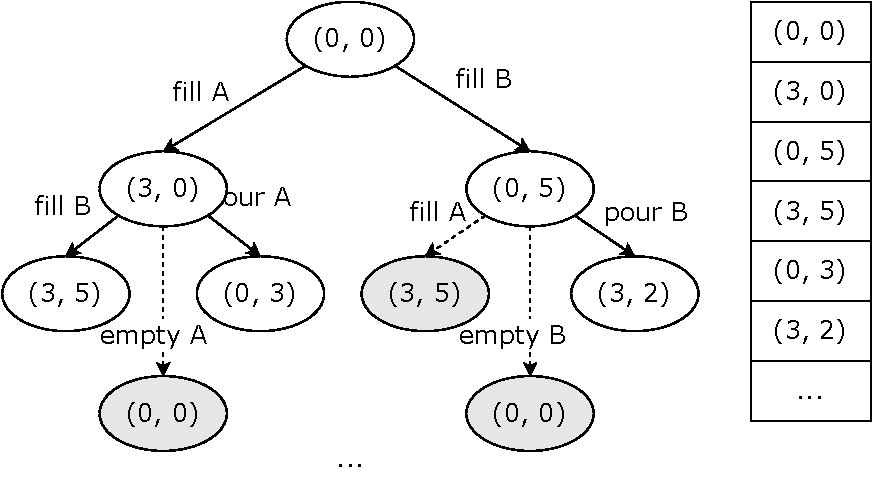
\includegraphics[scale=0.5]{img/water-jugs}
  \caption{全局列表}
  \label{fig:water-jugs}
\end{figure}

\begin{algorithmic}[1]
\Function{Solve}{$a, b, g$}
  \State $Q \gets \nil$
  \State \Call{Push-and-record}{$Q$, (0, 0)}
  \While{$Q \neq \nil$}
    \State $s \gets$ \Call{Pop}{$Q$}
    \If{$p(s) = g$ 或 $q(s) = g$}
      \State \Return $s$
    \Else
      \State $C \gets$ \Call{Expand}{$s$}
      \For{each $c$ in $C$}
        \If{$c \neq s$ 且 ($not$ \Call{Visited}{$c$})}
          \State \Call{Push-and-record}{$Q, c$}
        \EndIf
      \EndFor
    \EndIf
  \EndWhile
  \State \Return $\nil$
\EndFunction
\end{algorithmic}

其中\textproc{Push-and-record}将元素入队并记录入访问列表中。出队时并不删除元素,而是将队列头部向后移动。

\subsubsection{华容道}
\index{华容道}

传统玩具华容道是滑块类游戏,如图\ref{fig:klotski-cn}。国外称Kloski。滑块大小、布局会有不同。华容道有10个滑块,上面标有数字或者图案。最小的滑块大小为一个单位的正方形,最大的一块为$2 \times 2$单位。在棋盘下方的中间,有一个宽度为2个单位长的缺口。最大的一块代表曹操,其他的为刘备手下的五虎上将和士兵。游戏的目标是要通过滑动,将曹操移动到棋盘最下方逃走。图\ref{fig:klotski-jp}是日本游戏“箱子中的女儿”,最大的一块代表女儿,剩余滑块代表其他家庭成员。

\begin{figure}[htbp]
 \centering
 \subcaptionbox{起始布局}{\includegraphics[scale=0.5]{img/klotski-cn1}} \hspace{.01\textwidth}
 \subcaptionbox{移动若干步后的样子}{\includegraphics[scale=0.5]{img/klotski-cn2}}
 \caption{华容道游戏}
 \label{fig:klotski-cn}
\end{figure}

\begin{figure}[htbp]
 \centering
 \includegraphics[scale=0.5]{img/klotski-jp}
 \caption{日本的“箱子中的女儿”游戏}
 \label{fig:klotski-jp}
\end{figure}

我们用$5 \times 4$矩阵来代表棋盘,行列从0开始。1到10个数字代表棋子。0代表空位置。矩阵$M$给出了华容道的初始状态。值为$i$的格子表示有棋子占据。布局用字典$L$代表。$L[i]$棋子$i$覆盖的位置集合。例如$L[4] = \{(2, 1), (2, 2)\}$表示第4个棋子覆盖了位置$(2, 1)$、$(2, 2)$。我们可以把棋盘上的20个位置编号为0到19,把行列转化为编号:$c = 4y + x$。这样第四个棋子占据$L[4] = \{9, 10\}$。

\[
\begin{array}{cc}
M = \left [
  \begin{array}{cccc}
  1 & 10 & 10 & 2 \\
  1 & 10 & 10 & 2 \\
  3 & 4 & 4 & 5 \\
  3 & 7 & 8 & 5 \\
  6 & 0 & 0 & 9
  \end{array}
\right ] &
L = \left \{
  \begin{array}{l}
  1 \mapsto \{0, 4\}, 2 \mapsto \{3, 7\}, 3 \mapsto \{8, 12\}, \\
  4 \mapsto \{9, 10\}, 5 \mapsto \{11, 15\}, \\
  6 \mapsto \{16\}, 7 \mapsto \{ 13 \}, 8 \mapsto \{ 14 \}, \\
  9 \mapsto \{ 19 \}, 10 \mapsto \{1, 2, 5, 6\}
  \end{array}
\right \}
\end{array}
\]

我们可以定义映射$\varphi(M) \mapsto L$和逆映射$\varphi^{-1}(L) \mapsto M$在棋盘和布局间转换:

\begin{algorithmic}[1]
\Function{$\varphi$}{$M$}
  \State $L \gets \{ \}$
  \For{$y \gets 0 \sim 4$}
    \For{$x \gets 0 \sim 3$}
      \State $k \gets M[y][x]$
      \State $L[k] \gets$ \Call{Add}{$L[k], 4y + x$}
    \EndFor
  \EndFor
  \State \Return $L$
\EndFunction
\Statex
\Function{$\varphi^{-1}$}{$L$}
  \State $M \gets [[0] \times 4] \times 5$
  \For{each $(k \mapsto S)$ in $L$}
    \For{each $c$ in $S$}
      \State $x \gets c \bmod 4, y \gets \lfloor c / 4\rfloor$
      \State $M[y][x] \gets k$
    \EndFor
  \EndFor
  \State \Return $M$
\EndFunction
\end{algorithmic}

我们检查全部10个棋子,看看能否在上下左右4个方向移动1格。在矩阵棋盘上,移动表示为$(\Delta y, \Delta x) = (0, \pm 1), (\pm 1, 0)$,在布局上,四个方向分别表示为位移$d = \pm 1, \pm 4$,例如棋子$L[i] = \{c_1, c_2\}$向左移动变为$\{c_1 -1, c_2 -1\}$。这里要排除两个特殊情况:$d = 1, c \bmod 4 = 3$和$d = -1, c \bmod 4 = 0$,防止棋子从一侧边界跳到另一侧。考虑两个空位四周最多有8种移动可能。例如第一步只有4种可能:第6块向右;第7或第8块向下;第9块向左。图\ref{fig:klotski-valid-move}描述列如何检查移动可行。

\begin{figure}[htbp]
 \centering
 \includegraphics[scale=0.4]{img/klotski-valid-move}
 \caption{左侧:两个标1的格子都可移动;右侧:下方标1的格子和标2的格子冲突。}
 \label{fig:klotski-valid-move}
\end{figure}

为了确定可否移动,我们检查棋子$k$移动到的目标格子,如果为0或者$k$则可移动:

\be
\begin{array}{rl}
valid\ L[k]\ d: & \\
\forall c \in L[k] \Rightarrow & y = \lfloor c / 4 \rfloor + \lfloor d / 4 \rfloor, x = (c \bmod 4) + (d \bmod 4), \\
& (0, 0) \leq (y, x) \leq (4, 3), M[y][x] \in \{k, 0\}
\end{array}
\ee

经过一系列移动可能回到某个布局。仅避免棋盘矩阵相同是不够的,虽然下面的$M_1 \neq M_2$,但它们本质上是相同的布局。

\[
\begin{array}{cc}
M_1 = \left [
  \begin{array}{cccc}
  1 & 10 & 10 & 2 \\
  1 & 10 & 10 & 2 \\
  3 & 4 & 4 & 5 \\
  3 & 7 & 8 & 5 \\
  6 & 0 & 0 & 9
  \end{array}
\right ] &
M_2 = \left [
  \begin{array}{cccc}
  2 & 10 & 10 & 1 \\
  2 & 10 & 10 & 1 \\
  3 & 4 & 4 & 5 \\
  3 & 7 & 6 & 5 \\
  8 & 0 & 0 & 9
  \end{array}
\right ]
\end{array}
\]

我们需要比较布局来避免重复。忽略具体棋子,定义归一化布局为集合:$\|L\| = \{ p | (k \mapsto p) \in L\}$,也就是字典$L$中所有值的集合。上面两个矩阵的归一化布局都等于\{\{1, 2, 5, 6\}, \{0, 4\}, \{3, 7\}, \{8, 12\}, \{9, 10\}, \{11, 15\}, \{16\}, \{13\}, \{14\}, \{19\}\}。左右对称的布局也是一种重复,需要避免。例如下面的$M_1$和$M_2$对称。

\[
\begin{array}{cc}
M_1 = \left [
  \begin{array}{cccc}
  10 & 10 & 1 & 2 \\
  10 & 10 & 1 & 2 \\
  3 & 5 & 4 & 4 \\
  3 & 5 & 8 & 9 \\
  6 & 7 & 0 & 0
  \end{array}
\right ] &
M_2 = \left [
  \begin{array}{cccc}
  3 & 1 & 10 & 10 \\
  3 & 1 & 10 & 10 \\
  4 & 4 & 2 & 5 \\
  7 & 6 & 2 & 5 \\
  0 & 0 & 9 & 8
  \end{array}
\right ]
\end{array}
\]

它们的归一化布局也是对称的。我们定义归一化布局的对称变换:

\be
mirror(\|L\|) = \{\{ f(c) | c \in s \} | s \in \|L\|\}
\ee

其中$f(c) = 4y' + x', y' = \lfloor c / 4 \rfloor, x' = 3 - (c \bmod 4)$。我们使用一个队列进行搜索,队列中每个元素包含两部分:一系列移动和这些移动导致的布局。每次移动为$(k, d)$,表示在棋盘上移动棋子$k$,方向为$d$(值为$\pm 1, \pm 4$)。队列初始化为$Q = \{(s, [\ ])\}$,其中$s$是起始布局。只要$Q \neq \nil$,我们就从头部取出一个元素,检查最大的棋子(编号10)是否到达目标位置$t = \{13, 14, 17, 18\}$,即$L[10] = t$。如到达则结束;否则,我们尝试上下左右移动每块棋子,把所有可行的、不重复布的局移动方案$(k, d)$入队。在搜索过程中,我们用集合$H$记录归一化布局以避免重复。

\be
\begin{array}{rcl}
solve\ \nil\ H\ & = & [\ ] \\
solve\ Q\ H\ & = & \begin{cases}
  L[10] = t: & \textit{reverse}\ ms, \text{其中} ((L, ms), Q') = pop\ Q \\
  \text{否则}: & solve\ (pushAll\ cs\ Q')\ H' \\
  \end{cases}
\end{array}
\ee

其中$cs = [(move\ L\ e, e \cons ms) | e \gets expand\ L]$是新产生的移动方案。

\be
\begin{array}{rl}
expand\ L = \{(k, d) | & k \gets [1, 2, ..., 10], d \gets [\pm 1, \pm 4], \\
  &  valid\ k\ d, unique\ k\ d \} \\
\end{array}
\ee

$move$把棋子$L[k]$移动$d$成为:$move\ L\ (k, d) = map\ (+ d)\ L[k]$。$unique$判断新归一化布局$\|L'\| \notin H$,镜像$mirror(\|L'\|) \notin H$不在历史记录中。如果没有重复,更新它们到新记录$H'$用于后继搜索。下面是对应的迭代式实现。“横刀立马”布局的最少步数解共116步(每步移动1格),最后3步如下:

\begin{algorithmic}[1]
\Function{Solve}{$s, e$}
  \State $H \gets \{\|s\|\}$
  \State $Q \gets \{(s, \nil)\}$
  \While{$Q \neq \nil$}
    \State $(L, p) \gets$ \Call{Pop}{$Q$}
    \If{$L[10] = e$}
      \State \Return $(L, p)$
    \Else
      \For{each $L'$ in \Call{Expand}{$L, H$}}
        \State \Call{Push}{$Q, (L', L)$}
        \State \Call{Add}{$H, \|L'\|$}
      \EndFor
    \EndIf
  \EndWhile
  \State \Return $\nil$
\EndFunction
\end{algorithmic}

\begin{verbatim}

['5', '3', '2', '1']
['5', '3', '2', '1']
['7', '9', '4', '4']
['A', 'A', '6', '0']
['A', 'A', '0', '8']

['5', '3', '2', '1']
['5', '3', '2', '1']
['7', '9', '4', '4']
['A', 'A', '0', '6']
['A', 'A', '0', '8']

['5', '3', '2', '1']
['5', '3', '2', '1']
['7', '9', '4', '4']
['0', 'A', 'A', '6']
['0', 'A', 'A', '8']

\end{verbatim}

\index{BFS} \index{广度优先搜索}
过河问题、倒水问题、华容道游戏的解法有共同的结构。和深度优先类似,它们都有起始、终止状态。在过河问题中,起始状态是农夫、狼、羊、白菜在河的一岸,对岸为空;终止状态是全部渡河到了对岸。倒水问题的起始状态是两个空瓶子,而终止状态是某个瓶子盛有指定容量的水。华容道问题的起始状态是某种布局(“横刀立马”),终止状态是另外一个布局,其中最大的棋子移动到了指定的位置。每个问题都有相应的规则,可以从一个状态转移到另外一个状态。我们“并行”尝试可能选项。在同一步内的选项未尝试完之前,我们不会进一步深入搜索。这就保证了最小步骤解在其它解之前出现。由于向水平方向扩展,这种方法称为广度优先搜索。图\ref{fig:dfs-bfs-tree}给出了广度、深度优先搜索的对比。

\begin{figure}[htbp]
 \centering
 \subcaptionbox{深度优先搜索}{ \includegraphics[scale=0.45]{img/dfs-tree}}
 \subcaptionbox{广度优先搜索}{ \includegraphics[scale=0.45]{img/bfs-tree}}
 \caption{深度和广度优先搜索的顺序}
 \label{fig:dfs-bfs-tree}
\end{figure}

由于我们无法真正的“并行”搜索,广度优先搜索使用队列来记录尝试。从队列头部步骤不断取出较少的候选项,从队列尾部不断加入步骤较多的新候选项。广度优先搜索提供了一种简单的方法寻找最少步骤解,但它不能直接搜索其它最优解。考虑如图\ref{fig:weighted-dag}的有向图,每段路径长度不同,我们无法用广度优先搜索找出两个城市之间的最短路径。注意从城市$a$到城市$c$之间的最短路径并非经过最少城市的$a \to b \to c$。这条路径的总长度为22;而是经过更多城市的路径$a \to e \to f \to c$,他的总长度只有20。

\begin{figure}[htbp]
 \centering
 \includegraphics[scale=0.5]{img/weighted-dag}
 \caption{带权重的有向图}
 \label{fig:weighted-dag}
\end{figure}

\subsection{搜索最优解}

\index{贪心算法} \index{哈夫曼编码}
人们需要“最好”的解来节省时间、空间、成本、能量。使用有限的资源搜索最优解并不容易。有很多问题不存在多项式时间的解法。仅对一些特定问题存在简单方法找到最优解。哈夫曼编码是一种用最小长度对信息编码的方法。早期的ASCII码使用7位二进制数对字母、数字、符号编码,可以表达$2^7 = 128$个字符。只用0、1,我们至少需要$\log_2 n$位分辨$n$个不同字符。下面是大写英文字母的码表,将字母A到Z映射为0到25。每个编码5位。零被扩充到5位00000而非0。这样的编码方式称为定长编码。

\btab{l|l||l|l}
字符 & 编码 & 字符 & 编码 \\
\hline
A & 00000 & N & 01101 \\
B & 00001 & O & 01110 \\
C & 00010 & P & 01111 \\
D & 00011 & Q & 10000 \\
E & 00100 & R & 10001 \\
F & 00101 & S & 10010 \\
G & 00110 & T & 10011 \\
H & 00111 & U & 10100 \\
I & 01000 & V & 10101 \\
J & 01001 & W & 10110 \\
K & 01010 & X & 10111 \\
L & 01011 & Y & 11000 \\
M & 01100 & Z & 11001 \\
\hline
\etab

文本“INTERNATIONAL”可以编码为65位的二进制数:

\begin{Verbatim}[fontsize=\footnotesize]
00010101101100100100100011011000000110010001001110101100000011010
\end{Verbatim}

另一种方式是变长编码。用一位二进制数0代表A,用两位二进制数10代表C,用5位二进制数11001代表Z。虽然可以显著缩短编码长度。但在解码时会造成歧义。例如二进制数1101,我们不知道它是1,后面跟着101(表示“BF”),还是110,后面跟着1(表示“GB”),或是1101(表示N)。摩尔斯电码是变长编码。最常用的字符E编码为“.”,字符Z编码为“- -..”。使用特殊终止符分割编码,所以不会发生歧义。下面是一个特殊的无歧义码表:

\btab{l|l||l|l}
字符 & 编码 & 字符 & 编码 \\
\hline
A & 110 & E & 1110 \\
I & 101 & L & 1111 \\
N & 01 & O & 000 \\
R & 001 & T & 100 \\
\hline
\etab

文本“INTERNATIONAL”编码为38位的二进制数:

\begin{Verbatim}[fontsize=\footnotesize]
10101100111000101110100101000011101111
\end{Verbatim}

按上表解码不会遇到有歧义的字符。这是因为没有任何编码是其它编码的前缀。这样的编码称为\textbf{前缀码}\footnote{英文叫做prefix-code,而不是无前缀码.}。前缀码不需要分隔符,编码长度可进一步缩短。这自然引发了一个问题:给定文本,能否找到码表使得编码长度最短?1951年,麻省理工学院的学生大卫$\cdot$哈夫曼\cite{Huffman}的老师罗伯特$\cdot$费诺在课上宣布:谁解出了这个问题就不用参加期末考试了。哈夫曼尝试了很久。他几乎放弃了,开始准备考试。恰在此时,他灵光乍现找到了解法。哈夫曼根据文本中字符出现的频率构造码表。最“常见”的字符编码最短。首先处理文本获得每个字符出现的次数。定义字符的权重是它出现的次数或概率。哈夫曼用二叉树产生前缀码。字符保存于叶子节点。从根节点遍历产生编码。向左前进时添加0,向右前进时添加1,如图\ref{fig:huffman-tr}。例如,从根节点遍历到N的路径是,向左然后向右到达N。因此N编码为01;字符A的路径是:右、右,左,编码是110。

\begin{figure}[htbp]
 \centering
 \includegraphics[scale=0.5]{img/huffman-tr}
 \caption{哈夫曼树}
 \label{fig:huffman-tr}
\end{figure}

这棵树还可以解码。扫描二进制数,0向左、1向右。到达叶子时,节点上的字符就是解码内容。然后重新返回根节点继续扫描。哈夫曼用自底向上的方法构造树。开始时,每个字符都放入一个叶子节点中。每次选出两个权重最小的节点合并成一个分支。分支权重为两个子树的权重和。不断选择权重最小的两棵树合并,最后得到一棵树,如图\ref{fig:huffman-build}。

\captionsetup[subfigure]{labelformat=empty, margin=10pt}
\begin{figure}[htbp]
 \centering
 \subcaptionbox{第一步}{ \includegraphics[scale=0.4]{img/huffman-tr1}}
 \subcaptionbox{第二步}{ \includegraphics[scale=0.4]{img/huffman-tr2}}
 \subcaptionbox{第三步}{ \includegraphics[scale=0.4]{img/huffman-tr3}} \\
 \subcaptionbox{第四步}{ \includegraphics[scale=0.4]{img/huffman-tr4}}
 \subcaptionbox{第五步}{ \includegraphics[scale=0.4]{img/huffman-tr5}} \\
 \subcaptionbox{第六步}{ \includegraphics[scale=0.3]{img/huffman-tr6}} \\
 \subcaptionbox{第七步}{ \includegraphics[scale=0.3]{img/huffman-tr}}
 \caption{构造哈夫曼树}
 \label{fig:huffman-build}
\end{figure}
\captionsetup[subfigure]{labelformat=parens}

我们重用二叉树的定义实现哈夫曼树。节点中增加了权重,只有叶子节点保存字符。分枝节点表示为$(w, l, r)$,其中$w$是权重,$l, r$是左右子树。叶子节点表示为$(w, c)$其中$c$是字符。合并子树时,权重相加$merge\ a\ b\ = (weight\ a + weight\ b, a, b)$,其中:

\be
\begin{array}{rcl}
weight\ (w, a) & = & w \\
weight\ (w, l, r) & = & w \\
\end{array}
\ee

下面算法不断选出两棵权重最小的子树合并:

\be
\begin{array}{rcl}
build\ [t] & = & t \\
build\ ts & = & build\ (merge\ t_1 t_2)\ ts', \text{其中} (t_1, t_2, ts') = extract\ ts
\end{array}
\ee

函数$extract$从子树列表中选出权重最小的两棵树,若$weight\ t_1 < weight\ t_2$,定义$t_1 < t_2$。

\be
extract (t_1 \cons t_2 \cons ts) = foldr\ min_2\ (\min t_1\ t_2, \max t_1\ t_2, [\ ])\ ts
\ee

其中:

\be
min_2\ t\ (t_1, t_2, ts) = \begin{cases}
  t < t_2: & (\min\ t\ t_1, \max\ t\ t_1, t_2 \cons ts) \\
  \text{否则}: & (t_1, t_2, t \cons ts) \\
\end{cases}
\ee

为了迭代构造哈夫曼树,我们用数组$A$存储$n$棵子树。从右向左扫描$A$,如果$A[i]$的权重小于$A[n-1], A[n]$,就交换$A[i]$和\textproc{MAX}($A[n-1], A[n]$)。扫描后合并$A[n]$到$A[n-1]$。这样数组缩小一。重复此过程得到最终的哈夫曼树:

\begin{algorithmic}[1]
\Function{Huffman}{$A$}
  \While{$|A|>1$}
    \State $n \gets |A|$
    \For{$i \gets n - 2 $ down to $1$}
      \State $T \gets$ \Call{Max}{$A[n], A[n-1]$}
      \If{$A[i] < T$}
        \State \textproc{Exchange} $A[i]$ $\leftrightarrow T$
      \EndIf
    \EndFor
    \State $A[n-1] \gets$ \Call{Merge}{$A[n], A[n-1]$}
    \State \Call{Drop}{$A[n]$}
  \EndWhile
  \State \Return $A[1]$
\EndFunction
\end{algorithmic}

我们可以从哈夫曼树$T$构造码表。令$p = [\ ]$。从根节点遍历树。左转时$p \gets 0 \cons p$,右转时$p \gets 1 \cons p $。到达叶节点字符$c$时,记录$c \mapsto reverse\ p$到码表。定义(柯里化)$code\ = \textit{traverse}\ [\ ]$,其中:

\be
\begin{array}{rcl}
\textit{traverse}\ p\ (w, c)\ & = & [c \mapsto reverse\ p] \\
\textit{traverse}\ p\ (w, l, r)\ & = & \textit{traverse}\ (0 \cons p)\ l \doubleplus \textit{traverse}\ (1 \cons p)\ l \\
\end{array}
\ee

编码过程一边扫描文本$w$一边查询码表$dict$产生二进制序列:

\be
encode\ dict\ w = \textit{concatMap}\ (c \mapsto dict[c])\ w, \text{其中} dict = code\ T
\ee

解码过程相反,一边扫描二进制序列$bs$一边查询哈夫曼树。从根节点开始,0向左、1向右,到达叶子节点时输出字符$c$,然后回到根节点继续解码。$\textit{decode}\ bs\ T = lookup\ bs\ T$,其中:

\be
\begin{array}{rcl}
lookup\ [\ ]\ (w, c) & = & [c] \\
lookup\ bs\ (w, c) & = & c : lookup\ bs\ T \\
lookup\ (b \cons bs)\ (w, l, r) & = & lookup\ bs\ (\text{if}\ b = 0\ \text{then}\ l\ \text{else}\ r)
\end{array}
\ee

哈夫曼树的构造过程采取了一种特殊策略:每次合并有若干选项,总是选取权重最小的两棵树合并。这一系列\textbf{局部}最优选择,产生了全局最优的前缀编码。局部最优一般不产生全局最优解。哈夫曼编码是个例外。我们称这种每次选择局部最优选项的方法为\textbf{贪心}策略。贪心算法可以解决、简化很多问题。但判断贪心策略能否产生全局最优解并不容易。通用的形式化证明仍然是一个活跃的研究领域\cite{CLRS}。

\paragraph{换零钱问题}
\index{换零钱问题}

去其他国家前,我们经常要换汇。人们越来越多地使用信用卡了,信用卡很方便,买东西时可以不担心零钱问题。如果使用现金,旅行结束时,往往会剩余一些钱。有些钱币爱好者会把钱换成硬币,收集起来。有没有什么办法,能把指定数量的钱换成最少数量的硬币呢?

我们用美国的钱币系统作为例子。总共有5种不同面额的硬币:1美分、5美分、25美分、50美分、和1美元。1美元等于100美分。使用前面介绍的贪心方法,我们每次总挑选不超过余额的最大面值硬币。记硬币价值列表为$C = \{1, 5, 25, 50, 100\}$。给定任何钱数$X$,兑换硬币的方法可以定义如下。

\be
change(X, C) = \left \{
  \begin{array}
  {r@{\quad:\quad}l}
  \phi & X = 0 \\
  \{ c_m \} \cup change(X-c_m, C) & c_m = max(\{c \in C, c \leq X\})
  \end{array}
\right.
\ee

如果$C$按照降序排列,$c_m$就是第一个不大于$X$的硬币。如果要兑换1.42美元,这一函数会生成硬币列表:$\{100, 25, 5, 5, 5, 1, 1\}$。可以很容易地将这一列表变换为一组面值——数量对$\{(100, 1), (25, 1), (5, 3), (1, 2)\}$。也就是说,我们需要一枚1美元硬币、一枚25美分硬币、三枚5美分硬币、两枚1美分硬币。下面的Haskell例子程序实现了这一最少兑换算法。

\lstset{language=Haskell}
\begin{lstlisting}[style=Haskell]
solve x = assoc . change x where
  change 0 _ = []
  change x cs = let c = head $ filter (<= x) cs in c : change (x - c) cs

assoc = (map (\cs -> (head cs, length cs))) . group
\end{lstlisting} %$

这一程序假设硬币按照降序排列,例如:

\lstset{language=Haskell}
\begin{lstlisting}[style=Haskell]
solve 142 [100, 50, 25, 5, 1]
\end{lstlisting}

这一算法是尾递归的,他可以很容易地转换为命令式的循环。

\begin{algorithmic}[1]
\Function{Change}{$X, C$}
  \State $R \gets \phi$
  \While{$X \neq 0$}
    \State $c_m = max(\{c \in C, c \leq X\})$
    \State $R \gets \{c_m\} \cup R$
    \State $X \gets X - c_m$
  \EndWhile
  \State \Return $R$
\EndFunction
\end{algorithmic}

下面的Python例子程序实现了这一命令式算法,结果以一个字典输出。

\lstset{language=Python}
\begin{lstlisting}
def change(x, coins):
    cs = {}
    while x != 0:
        m = max([c for c in coins if c <= x])
        cs[m] = 1 + cs.setdefault(m, 0)
        x = x - m
    return cs
\end{lstlisting}

对于美国这样的硬币系统,贪心方法可以找到最优解。硬币的数量是最少的。幸运的是,贪心算法对于大多数国家的硬币系统都有效。但是也有一些例外。例如,假设某国的硬币体系中包含的币值为1、3、和4。如果要兑换价值为6的钱,最好的解是使用两个面值为3的硬币。但是,贪心方法给出的结果却是3枚硬币:一枚面值为4,两枚面值为1。这并非最优解。

\paragraph{贪心方法的小结}

如换零钱问题所示,贪心方法并不一定能给出最优解。为了找到最优解,我们需要使用后面将要介绍的动态规划方法。

但在实际中,贪心方法得出的解往往还是不错的。举例来说,折行(word-wrap)是现代编辑器、和浏览器等软件中常见的功能。如果文本太长,在一行显示不下,就在某些位置将其拆成若干行显示。使用折行功能,用户就无需在输入时人为加入换行符。虽然动态规划方法能够给出使用最少行的解,但是它过于复杂了。反之,贪心算法能够给出接近最优的折行方案,并且实现起来简单、高效。如下面的算法所示,给定文本$T$,每行不能超出宽度$W$,每个单词件的间隔为$s$。

\begin{algorithmic}[1]
\State $L \gets W$
\For{$w \in T$}
  \If{$|w| + s > L$}
    \State Insert line break
    \State $L \gets W - |w|$
  \Else
    \State $L \gets L - |w| - s$
  \EndIf
\EndFor
\end{algorithmic}

对文本中的每个词$w$,该算法使用贪心策略在一行中放入尽可能多的词直到超出行宽限制。很多文本处理软件使用了类似的算法来进行折行处理。

也有很多情况,我们必须要找到严格的最优解,而不是近似最优解。可以使用动态规划方法来解决此类问题。

\begin{Exercise}
\Question{使用堆来构造哈夫曼树:不断从堆顶取出两颗子树,合并后放回堆中。}
\Question{如果字符已按权重排序成列表$A$,存在一个线性时间的构造哈夫曼树的方法:用队列$Q$保存合并结果。不断从$Q$和$A$头部取出较小的树,合并后入队。处理完列表中所有树后,队列中将只剩下一棵树。即最终的哈夫曼树。请实现这一方法。}
\end{Exercise}

\begin{Answer}
\Question{使用堆来构造哈夫曼树:不断从堆顶取出两颗子树,合并后放回堆中。

\[
\textit{Huffman}\ H = \begin{cases}
  H = \nil: & \nil \\
  |H| = 1: & pop\ H \\
  \text{否则}: & \textit{Huffman}\ (push\ (merge\ t_a\ t_b)\ H'') \\
\end{cases}
\]

其中:$(t_a, H') = pop\ H, (t_b, H'') = pop\ H'$

\begin{algorithmic}[1]
\Function{Huffman}{$H$}
  \While{$|H| > 1$}
    \State $t_a \gets$ \Call{Pop}{$H$}
    \State $t_b \gets$ \Call{Pop}{$H$}
    \State \textproc{Push}($H$, \Call{Merge}{$t_a, t_b$})
  \EndWhile
  \State \Return \Call{Pop}{$H$}
\EndFunction
\end{algorithmic}
}
\Question{如果字符已按权重排序成列表$A$,存在一个线性时间的构造哈夫曼树的方法:用队列$Q$保存合并结果。不断从$Q$和$A$头部取出较小的树,合并后入队。处理完列表中所有树后,队列中将只剩下一棵树。即最终的哈夫曼树。请实现这一方法。

$\textit{Huffman}\ (t \cons ts) = build\ (t, (ts, \nil))$,其中:

\[
\begin{array}{rcl}
build\ (t, ([\ ], \nil)) & = & t \\
build\ (t, h) & = & build\ (extract\ (ts, push\ (merge\ t\ t')\ q)) \\
\end{array}
\]

其中:$(t', (ts, q)) = extract\ h$

\[
\begin{array}{rcl}
extract\ (t \cons ts, \nil)) & = & (t, (ts, \nil)) \\
extract\ ([\ ], q) & = & (t, ([\ ], q'), \text{其中}: (t, q') = pop\ q \\
extract\ (t \cons ts, q) & = & \begin{cases}
  t' < t: & (t', (t \cons ts, q')), \text{其中}: (t', q') = pop\ q \\
  t < t': & (t, (ts, q)) \\
  \end{cases}
\end{array}
\]

}
\end{Answer}

\subsubsection{动态规划}
\index{动态规划}

在介绍换零钱问题时,我们发现贪心方法有时无法得到最优解。对于任何的硬币体系,有没有一种方法,可以保证找到最优解呢?

假设我们找到了兑换价值为$X$的钱的最优方案。所需要的硬币保存在列表$C_m$中。我们可以将这些硬币分成两组,$C_1$和$C_2$。它们分别等于价值$X_1$和$X_2$。我们接下来要证明,$C_1$是兑换$X_1$的最优解,且$C_2$是兑换$X_2$的最优解。

\begin{proof}[证明]
对$X_1$,假设存在一个另一个更好的兑换方法$C_1'$,它比$C_1$需要的硬币数量更少。则兑换方法$C_1' \cup C_2$使用的硬币数量要少于$C_m$。这和$C_m$是兑换价值为$X$的钱的最优解相矛盾。同样,我们也可以证明$C_2$是兑换$X_2$的最优解。
\end{proof}

注意,相反的情况并不一定成立。如果我们任选一个值$Y < X$,将原最优兑换问题分解为两个子问题:寻找兑换$Y$的最优解,和寻找兑换$X - Y$的最优解。将这两个最优解合并起来,并不一定是兑换$X$的最优解。考虑这样的反例:有三种硬币,币值为1、2、和4。兑换价值为6的钱的最优解需要两枚硬币,一枚价值为2,另一枚价值为4。但是,如果将问题分解为两个子问题$6 = 3 + 3$,尽管每个子问题的最优兑换方案为$3 = 1 + 2$,即使用一枚价值为1、另一枚价值为2的硬币兑换3,但组合起来的方案需要使用4枚硬币1 + 2 + 1 + 2来兑换6。

如果一个最优化问题可以分解为若干子最优化问题,我们称它具备“最优化子结构”(optimal substructure)。兑换零钱问题,必须在硬币价值的基础上分解,而不能任意分解。

兑换零钱问题的最优化子结构可以表达如下。

\be
change(X) = \left \{
  \begin{array}
  {r@{\quad:\quad}l}
  \phi & X = 0 \\
  least(\{c \cup change(X-c) | c \in C, c \leq X\}) & otherwise
  \end{array}
\right.
\ee

对于任意硬币系统$C$,兑换价值为0的钱显然不需要任何硬币;否则,我们检查每一个不大于兑换值$X$的候选币值$c$,递归搜索兑换$X - c$的最优解;我们选择所有候选方案中,使用硬币最少的一个作为最终结果。

下面的Haskell例子程序实现了这一自顶向下的递归解法。

\lstset{language=Haskell}
\begin{lstlisting}[style=Haskell]
change _ 0 = []
change cs x = minimumBy (compare `on` length)
                [c:change cs (x - c) | c <- cs, c <= x]
\end{lstlisting}

给定输入\texttt{change [1, 2, 4] 6},即使用价值为1、2、和4的硬币,兑换价值为6的钱,这一程序可以给出正确的答案\texttt{[2, 4]}。尽管如此,它在解决使用美国硬币体系兑换1.42美元的问题时性能成为了瓶颈。在一台2.7GHz的CPU,拥有8G内存的计算机上,这一程序在15分钟内仍未得出结果。

造成性能问题的原因在于,在自顶向下递归求解中,有大量的重复计算。当计算$change(142)$时,它需要检查$change(141)$、$change(137)$、$change(117)$、$change(92)$、和$change(42)$。接着在计算$change(141)$时,它需要将这个值分别减去1、2、25、50、和100美分。这样,就会再次遇到137、117、92、和42这些值。搜索空间按照5的指数急速爆炸。

这和使用自顶向下的递归方法计算斐波那契序列非常相似。

\be
F_n = \left \{
  \begin{array}
  {r@{\quad:\quad}l}
  1 & n = 1 \lor n = 2 \\
  F_{n-1} + F_{n-2} & otherwise
  \end{array}
\right.
\ee

举例来说,当计算$F_8$的时候,我们需要递归计算$F_7$和$F_6$。而当在计算$F_7$时,我们需要再次计算$F_6$,以及$F_5$……展开的过程如下面的等式,每次展开,计算都加倍。相同的值被一遍一遍地重复计算。

\[
\begin{array}{rl}
F_8 = & F_7 + F_6 \\
   = & F_6 + F_5 + F_5 + F_4 \\
   = & F_5 + F_4 + F_4 + F_3 + F_4 + F_3 + F_3 + F_2 \\
   = & ...
\end{array}
\]

为了避免重复计算,我们可以在求斐波那契数的时候维护一个表格$F$。这个表格的前两个元素被填写为1,其他的元素都是空白。在自顶向下的递归计算中,如果需要计算$F_k$,我们首先检查表格中的第$k$个元素,如果不是空白,我们就直接使用表格中的值。否则,我们需要进一步计算。当计算出$F_k$的值后,我们将其保存入表格中,以用于后继的查找。

\begin{algorithmic}[1]
\State $F \gets \{1, 1, NIL, NIL, ...\}$
\Function{Fibonacci}{$n$}
  \If{$n > 2 \land F[n] = NIL$}
    \State $F[n] \gets$ \Call{Fibonacci}{$n-1$} $+$ \Call{Fibonacci}{$n-2$}
  \EndIf
  \State \Return $F[n]$
\EndFunction
\end{algorithmic}

使用类似的思路,我们可以得出一个新的自顶向下的兑换硬币方法。我们使用一个表格$T$来记录最优的兑换办法。开始的时候,所有的内容都为空白。在自顶向下的递归计算中,我们查询这个表格,寻找兑换较小价值钱的兑换方法。每当计算出新值的兑换方法后,我们都把它存入表格中。

\begin{algorithmic}[1]
\State $T \gets \{\phi, \phi, ...\}$
\Function{Change}{$X$}
  \If{$X > 0 \land T[X] = \phi$}
    \For{$c \in C$}
      \If{$c \leq X$}
        \State $C_m \gets \{c\} \cup$ \Call{Change}{$X-c$}
        \If{$T[X] = \phi \lor |C_m| < |T[X]|$}
          \State $T[X] \gets C_m$
        \EndIf
      \EndIf
    \EndFor
  \EndIf
  \State \Return $T[X]$
\EndFunction
\end{algorithmic}

兑换价值为0的钱,显然不需要任何硬币,所以解为空$\phi$。否则,我们查找$T[X]$获得兑换$X$的解。如果表格中这项为空,则需要递归计算。我们在$C$中逐一尝试所有币值不大于$X$的硬币,寻找子问题,即兑换价值为$X-c$的最优方法。在子问题的最优解基础上,我们再加上1枚价值为$c$的硬币,就获得了兑换$X$的最优解。然后,我们将此最优解保存在表格中的$T[X]$一项内。

下面的Python例子程序实现了这一算法,它仅使用8000毫秒就给出了兑换1.42美元的最优解。

\lstset{language=Python}
\begin{lstlisting}
tab = [[] for _ in range(1000)]

def change(x, cs):
    if x > 0 and tab[x] == []:
        for s in [[c] + change(x - c, cs) for c in cs if c <= x]:
            if tab[x] == [] or len(s) < len(tab[x]):
                tab[x] = s
    return tab[x]
\end{lstlisting}

另外一种计算斐波那契数的方法,是按照顺序$F_1, F_2, F_3, ..., F_n$来计算。这恰好是人们在依次写下斐波那契数时的顺序。

\begin{algorithmic}[1]
\Function{Fibo}{$n$}
  \State $F = \{1, 1, NIL, NIL, ...\}$
  \For{$i \gets 3$ to $n$}
    \State $F[i] \gets F[i-1] + F[i-2]$
  \EndFor
  \State \Return $F[n]$
\EndFunction
\end{algorithmic}

我们可以使用类似的思路来解决兑换硬币问题。从价值为0的钱开始,所需硬币为空,然后我们接着寻找如何兑换价值为1的钱。以美国硬币系统为例,我们可以使用1美分;接着对于价值为2、3、和4的钱,可以分别兑换为2枚1美分硬币、3枚1美分硬币、和4枚1美分硬币。此时保存最优解的列表内容如表\ref{tab:change-money}(a)所示。

\begin{table}[htbp]
\centering
\begin{tabular}{c||c|c|c|c|c|}
\hline
价值 & 0 & 1 & 2 & 3 & 4 \\
\hline
最优解 & $\phi$ & $\{1\}$ & $\{1, 1\}$ & $\{1, 1, 1\}$ & $\{1, 1, 1, 1\}$ \\
\hline
\end{tabular} \\
(a) 兑换价值为4美分以内的最优解列表 \\
\vspace{10pt}
\begin{tabular}{c||c|c|c|c|c|c|}
\hline
价值 & 0 & 1 & 2 & 3 & 4 & 5 \\
\hline
最优解 & $\phi$ & $\{1\}$ & $\{1, 1\}$ & $\{1, 1, 1\}$ & $\{1, 1, 1, 1\}$ & $\{ 5 \}$ \\
\hline
\end{tabular} \\
(b) 兑换价值为5美分以内的最优解列表 \\
\caption{兑换零钱的最优解列表} \label{tab:change-money}
\end{table}

当兑换价值为5的钱时,情况发生了变化。共有两个选择:再次使用一枚1美分的硬币,即使用5个1美分的硬币兑换;或者使用1枚5美分的硬币。显然后者所需的硬币更少。因此最优解表格的内容变为如表\ref{tab:change-money}(b)所示。

接下来,兑换价值为6的钱时,由于有两种硬币:1美分和5美分都不大于6,我们需要检查这2种选项。

\begin{itemize}
\item 如果选择使用1美分,我们接下来需要兑换剩余的价值5。由于我们已经在表格中记录了兑换5的最优解$\{ 5 \}$,使用1枚5美分硬币。这样我们就得到一个兑换价值为6的一个解$\{5, 1\}$;
\item 如果选择使用5美分,我们接下来需要兑换剩余的价值1。通过查表,我们发现兑换1的最优解$\{ 1 \}$,这样我们就得到了兑换价值为6的另外一个解$\{1, 5\}$。
\end{itemize}

恰巧两个选项获得解都只需要两枚硬币,我们可以选择任何一个作为最优解。原则上说,我们每次选择所需硬币最少的解填入表格中。

在任何一次迭代中,当寻找价值$i < X$的兑换方案时,我们逐一检查所有的币值。对于任何不大于$i$的硬币,我们从表格中查找项$T[i-c]$来获取子问题的解。用这一解所需的硬币再加上一枚硬币$c$,就是兑换$i$的一个方案选项。我们选择所需硬币最少的一个,记录到表格中。

下面的算法实现了这一自底向上的思路。

\begin{algorithmic}[1]
\Function{Change}{$X$}
  \State $T \gets \{ \phi, \phi, ... \}$
  \For{$i \gets 1$ to $X$}
    \For{$c \in C, c \leq i$}
      \If{$T[i] = \phi \lor 1 + |T[i - c]| < |T[i]|$}
        \State $T[i] \gets \{ c \} \cup T[i-c]$
      \EndIf
    \EndFor
  \EndFor
  \State \Return $T[X]$
\EndFunction
\end{algorithmic}

下面的Python例子程序实现了这一算法。

\lstset{language=Python}
\begin{lstlisting}
def changemk(x, cs):
    s = [[] for _ in range(x+1)]
    for i in range(1, x+1):
        for c in cs:
            if c <= i and (s[i] == [] or 1 + len(s[i-c]) < len(s[i])):
                s[i] = [c] + s[i-c]
    return s[x]
\end{lstlisting}

观察保存解的表格,会发现其中有大量重复的内容。

\begin{table}[htbp]
\centering
\begin{tabular}{c||c|c|c|c|c|c|}
\hline
价值 & 6 & 7 & 8 & 9 & 10 & ... \\
\hline
最优解 & $\{ 1, 5 \}$ & $\{1, 1, 5\}$ & $\{1, 1, 1, 5\}$ & $\{1, 1, 1, 1, 5\}$ & $\{ 5, 5 \}$ & ... \\
\hline
\end{tabular}
\caption{最优解的表格中存在重复内容} %\label{}
\end{table}

这是因为最优子问题的解,被完全复制到父问题的解中。为了减少空间的消耗,我们可以仅记录相对子问题变化的部分。对于兑换硬币问题,我们只需要记录下为了兑换$i$,所选择的那一枚硬币。

\begin{algorithmic}[1]
\Function{Change'}{$X$}
  \State $T \gets \{ 0, \infty, \infty, ... \}$
  \State $S \gets \{ NIL, NIL, ... \}$
  \For{$i \gets 1$ to $X$}
    \For{$c \in C, c \leq i$}
      \If{$1 + T[i - c] < T[i]$}
        \State $T[i] \gets 1 + T[i-c]$
        \State $S[i] \gets c$
      \EndIf
    \EndFor
  \EndFor
  \While{$X > 0$}
    \State \Call{Print}{$S[X]$}
    \State $X \gets X - S[X]$
  \EndWhile
\EndFunction
\end{algorithmic}

为了避免记录完整的兑换硬币列表,这一新算法使用了两个表格$T$和$S$。$T$记录了兑换价值0、1、2……所需的最少硬币数量,而$S$记录了最优解所选择的第一个币值。为了获得兑换$X$的完整硬币列表,第一个选择的硬币为$S[X]$,接下来的最优化子问题是兑换$X' = X - S[X]$。我们查询表格$S[X']$获得下一个硬币。我们不断查询最优化子问题所需选择的硬币,直到表格的最初位置。下面的Python例子程序实现了这一算法。

\lstset{language=Python}
\begin{lstlisting}
def chgmk(x, cs):
    cnt = [0] + [x+1] * x
    s = [0]
    for i in range(1, x+1):
        coin = 0
        for c in cs:
            if c <= i and 1 + cnt[i-c] < cnt[i]:
                cnt[i] = 1 + cnt[i-c]
                coin = c
        s.append(coin)
    r = []
    while x > 0:
        r.append(s[x])
        x = x - s[x]
    return r
\end{lstlisting}

给定需要兑换的值$n$,这一算法循环$n$次。每次迭代,算法最多检查全部的硬币。总体运行时间为$\Theta(nk)$,其中$k$是指定硬币系统中不同面值硬币的数量。最后改进的算法,需要额外$O(n)$的空间。它使用表格$T$和$S$来记录最优化子问题的解。

在纯函数式的环境中,我们无法更改记录解的表格,或者在常数时间内查询。一种办法是使用前面章节介绍的finger树\footnote{某些纯函数式编程环境,如Haskell,提供了内置的数组;而其他的一些近似纯函数式环境,如ML,提供了可改变的数组。}。我们可以把所需的最少硬币数,和选择的硬币成对保存在树中。

记录最优解的表格,实际上为一棵finger树,它初始为$T = \{(0, 0)\}$。表示兑换价值为0的钱,无需任何硬币。我们对列表$\{1, 2, ..., X\}$进行fold,传入初始表格。fold使用的二元函数是$change(T, i)$。fold结束后,我们获得最终的最优解表格,然后再通过函数$make(X, T)$,从这一表格构造出兑换硬币的列表。

\be
makeChange(X) = make(X, fold(change, \{(0, 0)\}, \{1, 2, ..., X\}))
\ee

在函数$change(T, i)$中,我们检查所有价值不大于$i$的硬币,选出导致最优解的一个。所需硬币的最少数量,和选中的硬币组成一对值,插入到finger树中,最后返回新的表格作为结果。

\be
change(T, i) = insert(T, fold(sel, (\infty, 0), \{c | c \in C, c \leq i\}))
\ee

我们再次使用fold来选择硬币数最少的兑换方案。fold起始时的值为$(\infty, 0)$,列表为所有面值不大于$i$的硬币。函数$sel((n, c), c')$接受两个参数,第一个参数是一对值,包含所需硬币数量和选中的硬币。它是目前为止找到的最优解;另一个参数是一枚新硬币,我们需要检查这枚新硬币是否可以导致更好的解。

\be
sel((n, c), c') = \left \{
  \begin{array}
  {r@{\quad:\quad}l}
  (1 + n', c') & 1 + n' < n, (n', c') = T[i-c'] \\
  (n, c) & otherwise
  \end{array}
\right.
\ee

构造好最优解表格后,兑换所需的所有硬币就可以通过它逐一找出。

\be
make(X, T) = \left \{
  \begin{array}
  {r@{\quad:\quad}l}
  \phi & X = 0 \\
  \{c\} \cup make(X-c, T) & (n, c) = T[X]
  \end{array}
\right.
\ee

下面的Haskell例子程序实现了兑换硬币算法。它使用了标准库中的\texttt{Data.Sequence},其实现为finger树。

\lstset{language=Haskell}
\begin{lstlisting}[style=Haskell]
import Data.Sequence (Seq, singleton, index, (|>))

changemk x cs = makeChange x $ foldl change (singleton (0, 0)) [1..x] where
  change tab i = let sel c = min (1 + fst (index tab (i - c)), c)
                 in tab |> (foldr sel ((x + 1), 0) $ filter (<=i) cs)
  makeChange 0 _ = []
  makeChange x tab = let c = snd $ index tab x in c : makeChange (x - c) tab
\end{lstlisting} %$

不管是自底向上的方法,还是自顶向下的方法,都需要记录最优化子问题的解。这是因为在计算整体的最优解时,需要反复多次使用子问题的结果。这一特性称为重叠子问题(overlapping sub problems)。

\paragraph{动态规划的性质}

动态规划最早在1940年代由Richard Bellman提出。它是搜索最优解的有利武器,它要求问题要具备两个性质。

\begin{itemize}
\item 最优化子结构。问题可以被分解为若干规模较小的子问题,最优解可以高效地从这些子问题的解中构造出来;
\item 重叠子问题。问题可以被分解为若干子问题,子问题的解被多次反复使用以寻找整体上的解。
\end{itemize}

兑换硬币问题,同时拥有最优化子结构和重叠子问题的性质。

\paragraph{最长公共子序列问题}
\index{LCS} \index{最长公共子序列问题}

最长公共子序列问题和最长公共子串问题不同。在后缀树一章中,我们给出了如何寻找最长公共子串的方法。最长公共子序列无需是原序列中的连续部分。

例如,文本“Mississippi”和“Missunderstanding”的最长公共子串为“Miss”,而最长公共子序列为“Misssi”。如图\ref{fig:lcs}所示。

\begin{figure}[htbp]
 \centering
 \includegraphics[scale=0.3]{img/lcs}
 \caption{最长公共子序列}
 \label{fig:lcs}
\end{figure}

如果我们将这张图旋转90度,然后考虑这两段文本代表两段代码,它就变成了代码间比较“diff”的结果。大多数现在版本控制工具需要计算不同版本间的差异。最长公共子序列问题在其中扮演了重要的角色。

如果两个字符串$X$和$Y$中的任何一个为空,则最长公共子序列$LCS(X, Y)$也显然为空。否则,记$X = \{x_1, x_2, ..., x_n\}$、$Y = \{y_1, y_2, ..., y_m \}$。如果第一个元素$x_1$和$y_1$相同,我们可以递归地搜索$X' = \{x_2, x_3, ..., x_n \}$和$Y' = \{y_2, y_3, ..., y_m \}$的最长公共子序列。最终结果$LCS(X, Y)$可以通过将$x_1$附加到$LCS(X', Y')$之前获得。否则,若$x_1 \neq y_1$,我们需要递归搜索$LCS(X, Y')$和$LCS(X', Y)$的结果,选择较长的一个作为最终结果。综合这三种情况,我们可以得到下面的定义。

\be
LCS(X, Y) = \left \{
  \begin{array}
  {r@{\quad:\quad}l}
  \phi & X = \phi \lor Y = \phi \\
  \{x_1\} \cup LCS(X', Y') & x_1 = y_1 \\
  longer(LCS(X, Y'), LCS(X', Y)) & otherwise
  \end{array}
\right.
\ee

这一定义中含有明显的最优化子结构,最长公共子序列问题可以分解为规模较小的子问题。子问题至少比原问题的字符串长度短1。

同样,这一定义中也含有重叠子问题。子串间的最长公共子序列被多次用于搜索全局最优解。

由于存在这两个性质,我们可以使用动态规划来解决这一问题。

我们可以使用一个二维表格来记录子问题的最优解。行和列分别代表$X$和$Y$的子串。

\begin{table}[htbp]
\centering
\begin{tabular}{|c|c|c|c|c|c|c|c|c|}
\hline
 & & a & n & t & e & n & n & a \\
\hline
 & & 1 & 2 & 3 & 4 & 5 & 6 & 7 \\
\hline
b & 1 & & & & & & & \\
\hline
a & 2 & & & & & & & \\
\hline
n & 3 & & & & & & & \\
\hline
a & 4 & & & & & & & \\
\hline
n & 5 & & & & & & & \\
\hline
a & 6 & & & & & & & \\
\hline
\end{tabular}
\caption{记录最优解的二维表格} %\label{}
\end{table}

这一表格给出了求字符串“antenna”和“banana”之间最长公共子序列的例子。两个字符串的长度分别为7和6.我们首先检查表格的右下角,由于这一项为空,我们需要比较“antenna”中的第7个字符,和“banana”中的第6个字符。它们都是字符‘a’,我们接下来要递归查找第5行、第6列。这一项也为空,我们需要重复这一过程,直到达到边界情况,即一个字符串变为空,或者我们查找的表格中的一项已填入信息。同兑换硬币问题类似,当某一子问题的最优解被找到后,它被记录到表格中用于后继的查找。这一过程和递归定义相比,顺序是相反的,我们从每个字符串中最右侧的字符开始处理。

考虑空串和任何字符串的最长公共子序列也为空,我们可以扩展上述表格,使得第一行和第一列包含空字符串。

\begin{table}[htbp]
\centering
\begin{tabular}{|c|c|c|c|c|c|c|c|c|}
\hline
 & & a & n & t & e & n & n & a \\
\hline
 & & $\phi$ & $\phi$ & $\phi$ & $\phi$ & $\phi$ & $\phi$ & $\phi$ \\
\hline
b & $\phi$ & & & & & & & \\
\hline
a & $\phi$ & & & & & & & \\
\hline
n & $\phi$ & & & & & & & \\
\hline
a & $\phi$ & & & & & & & \\
\hline
n & $\phi$ & & & & & & & \\
\hline
a & $\phi$ & & & & & & & \\
\hline
\end{tabular}
\caption{包含空串的最优解表格}
\end{table}

下面的算法通过使用这样的表格,实现了自顶向下的动态规划解法。

\begin{algorithmic}[1]
\State $T \gets$ NIL
\Function{LCS}{$X, Y$}
  \State $m \gets |X|, n \gets |Y|$
  \State $m' \gets m+1, n' \gets n+1$
  \If{$T =$ NIL}
    \State $T \gets \{\{\phi, \phi, ..., \phi\}, \{\phi, NIL, NIL, ...\}, ...\}$ \Comment{$m' \times n'$}
  \EndIf
  \If{$X \neq \phi \land Y \neq \phi \land T[m'][n'] =$ NIL}
    \If{$X[m] = Y[n]$}
      \State $T[m'][n'] \gets$ \textproc{Append}(\Call{LCS}{$X[1...m-1], Y[1...n-1]$}, $X[m]$)
    \Else
      \State $T[m'][n'] \gets$ \textproc{Longer}(\Call{LCS}{$X, Y[1...n-1]$}, \Call{LCS}{$X[1...m-1], Y$})
    \EndIf
  \EndIf
  \State \Return $T[m'][n']$
\EndFunction
\end{algorithmic}

表格初始化时,第一行和第一列都被填入空串;剩余的项都为NIL。除非任何一个字符串为空,或者表格中的项不为NIL,我们比较两个字符串中的最后一个元素,并且递归计算子串间的最长公共子序列。下面的Python例子程序实现了这一算法。

\lstset{language=Python}
\begin{lstlisting}
def lcs(xs, ys):
    m = len(xs)
    n = len(ys)
    global tab
    if tab is None:
        tab = [[""]*(n+1)] + [[""] + [None]*n for _ in xrange(m)]
    if m != 0 and n !=0 and tab[m][n] is None:
        if xs[-1] == ys[-1]:
            tab[m][n] = lcs(xs[:-1], ys[:-1]) + xs[-1]
        else:
            (a, b) = (lcs(xs, ys[:-1]), lcs(xs[:-1], ys))
            tab[m][n] = a if len(b) < len(a) else b
    return tab[m][n]
\end{lstlisting}

也可以用自底向上的方法寻找最长公共子序列。思路和兑换硬币问题类似。另外,我们还可以避免在表格中保存完整的序列内容,而只存储最长子序列的长度,并最终从表格中构造出最长公共子序列。一开始时,表格中的所有项都初始化为0。

\begin{algorithmic}[1]
\Function{LCS}{$X, Y$}
  \State $m \gets |X|, n \gets |Y|$
  \State $T \gets \{\{0, 0, ...\}, \{0, 0, ...\}, ...\}$ \Comment{$(m+1) \times (n+1)$}
  \For{$i \gets 1$ to $m$}
    \For{$j \gets 1$ to $n$}
      \If{$X[i] = Y[j]$}
        \State $T[i+1][j+1] \gets T[i][j] + 1$
      \Else
        \State $T[i+1][j+1] \gets$ \Call{Max}{$T[i][j+1], T[i+1][j]$}
      \EndIf
    \EndFor
  \EndFor
  \State \Return \Call{Get}{$T, X, Y, m, n$}
\EndFunction
\Statex
\Function{Get}{$T, X, Y, i, j$}
  \If{$i = 0 \lor j = 0$}
    \State \Return $\phi$
  \ElsIf{$X[i] = Y[j]$}
    \State \Return \textproc{Append}(\Call{Get}{$T, X, Y, i-1, j-1$}, $X[i]$)
  \ElsIf{$T[i-1][j] > T[i][j-1]$}
    \State \Return \Call{Get}{$T, X, Y, i-1, j$}
  \Else
    \State \Return \Call{Get}{$T, X, Y, i, j-1$}
  \EndIf
\EndFunction
\end{algorithmic}

自底向上的搜索时,我们从第2行、第2列开始。这一项对应$X$和$Y$中的第1个元素。如果它们相等,则目前为止的最长公共子序列的长度为1。这可以通过将空串的长度加1得到。而空串的结果,存储在左上角上。否则,如果第一个元素不等,我们从表格正上方的一项和左方的一项中挑选较大的值填入。重复这一步骤,最终填完表格。

此后,我们进行回溯以构造出最长公共子序列。从表格的右下方开始。如果$X$和$Y$中最后一个元素相等,我们就把它作为结果中的最后一个元素,并沿着对角线方向继续查表。否则,如果最后一个元素不等,我们需要比较左侧和上方的项,选择值较大的继续进行处理。

下面的Python例子程序实现了这一算法。

\lstset{language=Python}
\begin{lstlisting}
def lcs(xs, ys):
    m = len(xs)
    n = len(ys)
    c = [[0]*(n+1) for _ in xrange(m+1)]
    for i in xrange(1, m+1):
        for j in xrange(1, n+1):
            if xs[i-1] == ys[j-1]:
                c[i][j] = c[i-1][j-1] + 1
            else:
                c[i][j] = max(c[i-1][j], c[i][j-1])

    return get(c, xs, ys, m, n)

def get(c, xs, ys, i, j):
    if i==0 or j==0:
        return []
    elif xs[i-1] == ys[j-1]:
        return get(c, xs, ys, i-1, j-1) + [xs[i-1]]
    elif c[i-1][j] > c[i][j-1]:
        return get(c, xs, ys, i-1, j)
    else:
        return get(c, xs, ys, i, j-1)
\end{lstlisting}

也可以用纯函数式的方法定义自底向上的动态规划解法。我们还是用finger树作为表格。第一行填入$n+1$个0。通过对序列$X$进行fold来构造表格。然后再从表格中构造最长公共子序列。

\be
LCS(X, Y) = construct(fold(f, \{\{0, 0, ..., 0\}\}, zip(\{1, 2, ...\}, X)))
\ee

由于需要按照索引查表,我们将$X$和自然数zip到一起。函数$f$通过对$Y$进行fold,创建表格中新的一行,并记录下目前为止,所有情况下最长公共子序列的长度。

\be
f(T, (i, x)) = insert(T, fold(longest, \{0\}, zip(\{1, 2, ...\}, Y)))
\ee

函数$longest$接受两个参数,第一个参数是目前为止表格中这一行已填入的内容,第二个参数是一对值,包含一个索引和$Y$中对应的元素。它比较这一元素和$X$中是否相同,并将较长的长度添加到这一行中。

\be
longest(R, (j, y)) = \left \{
  \begin{array}
  {r@{\quad:\quad}l}
  insert(R, 1 + T[i-1][j-1]  ) & x = y \\
  insert(R, max(T[i-1][j], T[i][j-1])) & otherwise
  \end{array}
\right.
\ee

表格构建完成后,可以通过查表构造出最长公共子序列。为了提高效率,我们可以传入反转的序列$\overleftarrow{X}$和$\overleftarrow{Y}$,以及他们各自的长度$m$和$n$。

\be
construct(T) = get((\overleftarrow{X}, m), (\overleftarrow{Y}, n))
\ee

如果序列不为空,记两个序列中的第一个元素分别为$x$和$y$。剩余的部分记为$\overleftarrow{X}'$和$\overleftarrow{Y}'$。函数$get$的具体定义如下。

\be
get((\overleftarrow{X}, i), (\overleftarrow{Y}, j)) = \left \{
  \begin{array}
  {r@{\quad:\quad}l}
  \phi & \overleftarrow{X} = \phi \land \overleftarrow{Y} = \phi \\
  get((\overleftarrow{X}', i-1), (\overleftarrow{Y}', j-1)) \cup \{x\} & x = y \\
  get((\overleftarrow{X}', i-1), (\overleftarrow{Y}, j)) & T[i-1][j] > T[i][j-1] \\
  get((\overleftarrow{X}, i), (\overleftarrow{Y}', j-1)) & otherwise
  \end{array}
\right.
\ee

下面的Haskell例子程序实现了这一算法。

\lstset{language=Haskell}
\begin{lstlisting}[style=Haskell]
lcs' xs ys = construct $ foldl f (singleton $ fromList $ replicate (n+1) 0)
                               (zip [1..] xs) where
  (m, n) = (length xs, length ys)
  f tab (i, x) = tab |> (foldl longer (singleton 0) (zip [1..] ys)) where
    longer r (j, y) = r |> if x == y
                    then 1 + (tab `index` (i-1) `index` (j-1))
                    else max (tab `index` (i-1) `index` j) (r `index` (j-1))
  construct tab = get (reverse xs, m) (reverse ys, n) where
    get ([], 0) ([], 0) = []
    get ((x:xs), i) ((y:ys), j)
      | x == y = get (xs, i-1) (ys, j-1) ++ [x]
      | (tab `index` (i-1) `index` j) > (tab `index` i `index` (j-1)) =
                 get (xs, i-1) ((y:ys), j)
      | otherwise = get ((x:xs), i) (ys, j-1)
\end{lstlisting}

\paragraph{子集和问题}
\index{子集和问题}

动态规划不仅可以解决最优化问题,还可以解决一些更为一般的搜索问题。例如子集和(subset sum)问题。给定若干整数的集合,是否存在一个非空子集,使得子集中元素相加的结果为0?例如集合$\{11, 64, -82, -68, 86, 55, -88, -21, 51\}$存在两个和为0的非空子集。一个是$\{64, -82, 55, -88, 51\}$,另一个是$\{64, -82, -68, 86\}$。

当然0是一个特殊的情况,有时我们需要找到一个子集,使得其和为某一给定值$s$。本节中,我们要找到所有满足的子集。

显然,暴力穷举法可以找到所有的解。对于每个元素,我们可以选择或者排除它,因此对于有$n$个元素的集合,总共有$2^n$个选项。对于每个选项,我们都需要检查和是否为$s$。累加是一个线性操作。因此总体上的复杂度为$O(n2^n)$。这是一个指数级的算法,如果集合中含有很多元素,所需时间会急速增加。

子集和问题存在一个递归解。如果集合为空,显然无解;否则,令集合为$X = \{x_1, x_2, ...\}$。若$x_1 = s$,则子集$\{x_1\}$是一个解,我们接着需要搜索集合的剩余部分$X' = \{x_2, x_3, ...\}$中是否仍有子集的和为$s$。否则,若$x_1 \neq s$,则存在两种可能性。我们既需要在$X'$中搜索子集和$s$,也需要搜索子集和$s - x_1$。对于任何和为$s - x_1$的子集,我们可以将$x_1$加入集合,构成一个新的解。下面的定义总结了上述的所有情况。

\be
solve(X, s) = \left \{
  \begin{array}
  {r@{\quad:\quad}l}
  \phi & X = \phi \\
  \{\{x_1\}\} \cup solve(X', s) & x_1 = s \\
  solve(X', s) \cup \{ \{x_1\} \cup S | S \in solve(X', s-x_1)\} & otherwise
  \end{array}
\right.
\ee

这一定义明显含有子结构,虽然它不是最优化子结构。并且,这一定义也含有重叠子问题。我们可以用动态规划的思路,使用一张表来记录子问题的解,从而解决子集和问题。

在输出所有满足的子集内容前,我们首先考虑如何解决判定问题。当存在某一子集和为$s$,则输出“存在”,否则输出“不存在”。

通过一轮扫描我们可以确定子集和的上下限。如果指定的和$s$不在上下限确定的范围内,则显然无解。

\be
\left \{
  \begin{array}{l}
  s_l = \sum \{x \in X, x < 0\} \\
  s_u = \sum \{x \in X, x > 0\}
  \end{array}
\right.
\ee

否则,若$s_l \leq s \leq s_u$,由于所有的元素都是整数,我们可以使用一张表格,含有$s_u - s_l + 1$列,每列代表这一范围内的一个可能的值,从$s_l$到$s_u$。表格中每项的内容为真或假,表示是否存在一个子集,其和为该项对应的值。开始的时候,所有的项都初始化为假。我们从集合$X$中的第一个元素$x_1$开始,显然子集$\{x_1\}$的和为$x_1$,所以表格第一行中代表$x_1$的一项应为真。

\begin{table}[htbp]
\centering
\begin{tabular}{|c|c|c|c|c|c|c|}
\hline
 & $s_l$ & $s_l+1$ & ... & $x_1$ & ... & $s_u$ \\
\hline
$x_1$ & F & F & ... & T & ... & F \\
\hline
\end{tabular}
\caption{子集和问题的解表格第一行}
\end{table}

使用集合中的第二个元素$x_2$,可以得到3种可能的和。和第一行类似,子集$\{x_2\}$的和为$x_2$;对于前一行中所有可能值,如果不加上$x_2$,它们作为子集和仍然可以得到,所以第一行中$x_1$下面的一项也应该为真;通过将$x_2$加到所有可能的和之上,我们可以得到一些新值。因此代表$x_1 + x_2$的一项应为真。

\begin{table}[htbp]
\centering
\begin{tabular}{|c|c|c|c|c|c|c|c|c|c|c|}
\hline
 & $s_l$ & $s_l+1$ & ... & $x_1$ & ... & $x_2$ & ... & $x_1 + x_2$ & ... & $s_u$ \\
\hline
$x_1$ & F & F & ... & T & ... & F & ... & F & ... & F \\
\hline
$x_2$ & F & F & ... & T & ... & T & ... & T & ... & F \\
\hline
\end{tabular}
\caption{子集和问题的解表格第二行}
\end{table}

总而言之,当填写表格第$i$行的时候,所有由$\{x_1, x_2, ..., x_{i-1}\}$可获得的和,仍然可以获得。因此上一行中为真的项,仍然为真。对应值为$x_i$的一项应为真,因为只含有一个元素的集合$\{x_i\}$的和为$x_i$。我们可以将$x_i$加到已知的所有和之上,这样可以得到一些新值,对应这些新值的项也应为真。

当这样处理完所有的元素后,我们得到了一个含有$|X|$行的表格。通过查询最后一行,对应值为$s$的项是真还是假,就可以知道是否存在子集的和为$s$。由于$s < s_l$或$s_u < s$时无解,在这种情况下可以跳过表格的构造过程。我们暂时略过这一错误处理。

\begin{algorithmic}[1]
\Function{Subset-Sum}{$X, s$}
  \State $s_l \gets \sum \{x \in X, x < 0\}$
  \State $s_u \gets \sum \{x \in X, x > 0\}$
  \State $n \gets |X|$
  \State $T \gets \{\{False, False, ...\}, \{False, False, ...\}, ...\}$ \Comment{$n \times (s_u - s_l + 1)$}
  \For{$i \gets 1$ to $n$}
    \For{$j \gets s_l$ to $s_u$}
      \If{$X[i] = j$}
        \State $T[i][j] \gets True$
      \EndIf
      \If{$i > 1$}
        \State $T[i][j] \gets T[i][j] \lor T[i-1][j]$
        \State $j' \gets j - X[i]$
        \If{$s_l \leq j' \leq s_u$}
          \State $T[i][j] \gets T[i][j] \lor T[i-1][j']$
        \EndIf
      \EndIf
    \EndFor
  \EndFor
  \State \Return $T[n][s]$
\EndFunction
\end{algorithmic}

注意,表格中列的索引不是从1到$s_u-s_l + 1$,而是从$s_l$到$s_u$。由于大多数编程环境不支持负索引,我们可以通过$T[i][j-s_l]$来进行换算。下面的Python例子程序使用了负索引的特性。

\lstset{language=Python}
\begin{lstlisting}
def solve(xs, s):
    low = sum([x for x in xs if x < 0])
    up  = sum([x for x in xs if x > 0])
    tab = [[False]*(up-low+1) for _ in xs]
    for i in xrange(0, len(xs)):
        for j in xrange(low, up+1):
            tab[i][j] = (xs[i] == j)
            j1 = j - xs[i];
            tab[i][j] = tab[i][j] or tab[i-1][j] or
                        (low <= j1 and j1 <= up and tab[i-1][j1])
    return tab[-1][s]
\end{lstlisting}

这一程序没有使用单独的分支来处理$i = 0$和$i = 1, 2, ..., n-1$的不同情况。这是因为$i = 0$时,行的索引$i - 1 = -1$,它指向表格中的最后一行,其中的值都为假。这样就简化了程序的逻辑。

使用这一表格,可以很容易地构建出所有和为$s$的子集。首先查询表格中最后一行代表$s$的一项。如果最后一个元素$x_n = s$,则子集$\{x_n\}$显然是一个解。我们接下来查找上一行中$s$对应的项,并递归地从$\{x_1, x_2, x_3, ..., x_{n-1}\}$中构造所有和为$s$的子集。最后,我们检查倒数第二行,对应$s - x_n$的项。对于所有和为这一值的子集,我们加入$x_n$后构造一个新的集合,其和为$s$。

\begin{algorithmic}[1]
\Function{Get}{$X, s, T, n$}
  \State $S \gets \phi$
  \If{$X[n] = s$}
    \State $S \gets S \cup \{X[n]\}$
  \EndIf
  \If{$n > 1$}
    \If{$T[n-1][s]$}
      \State $S \gets S \cup $ \Call{Get}{$X, s, T, n-1$}
    \EndIf
    \If{$T[n-1][s-X[n]]$}
      \State $S \gets S \cup \{\{X[n]\} \cup S' | S' \in $ \Call{Get}{$X, s-X[n], T, n-1$} $\}$
    \EndIf
  \EndIf
  \State \Return $S$
\EndFunction
\end{algorithmic}

下面的Python例子程序实现了这一算法。

\lstset{language=Python}
\begin{lstlisting}
def get(xs, s, tab, n):
    r = []
    if xs[n] == s:
        r.append([xs[n]])
    if n > 0:
        if tab[n-1][s]:
            r = r + get(xs, s, tab, n-1)
        if tab[n-1][s - xs[n]]:
            r = r + [[xs[n]] + ys for ys in get(xs, s - xs[n], tab, n-1)]
    return r
\end{lstlisting}

这一子集和问题的动态规划解法循环了$O(n(s_u - s_l + 1))$次以构建表格,然后递归$O(n)$次从这一表格构造最后的解。它所用的空间也为$O(n(s_u - s_l + 1))$。

我们可以使用一个向量来代替含有$n$行的表格。向量中的每一项对应一个可能的和,其中存储了子集的列表。开始时,向量中的所有项都为空。对于$X$中的每一个元素,我们不断更新向量,它记录了所有可能得到的和。当所有的元素都处理完毕后,对应$s$的那一项包含了最终的答案。

\begin{algorithmic}[1]
\Function{Subset-Sum}{$X, s$}
  \State $s_l \gets \sum \{x \in X, x < 0\}$
  \State $s_u \gets \sum \{x \in X, x > 0\}$
  \State $T \gets \{\phi, \phi, ...\}$ \Comment{$s_u - s_l + 1$}
  \For{$x \in X$}
    \State $T' \gets$ \Call{Duplicate}{$T$}
    \For{$j \gets s_l$ to $s_u$}
      \State $j' \gets j - x$
      \If{$x = j$}
        \State $T'[j] \gets T'[j] \cup \{x\}$
      \EndIf
      \If{$s_l \leq j' \leq s_u \land T[j'] \neq \phi$}
        \State $T'[j] \gets T'[j] \cup \{\{x\} \cup S | S \in T[j']\}$
      \EndIf
    \EndFor
    \State $T \gets T'$
  \EndFor
  \State \Return $T[s]$
\EndFunction
\end{algorithmic}

下面的Python例子程序实现了这一改进的算法。

\lstset{language=Python}
\begin{lstlisting}
def subsetsum(xs, s):
    low = sum([x for x in xs if x < 0])
    up  = sum([x for x in xs if x > 0])
    tab = [[] for _ in xrange(low, up+1)]
    for x in xs:
        tab1 = tab[:]
        for j in xrange(low, up+1):
            if x == j:
                tab1[j].append([x])
            j1 = j - x
            if low <= j1 and j1 <= up and tab[j1] != []:
                tab1[j] = tab1[j] + [[x] + ys for ys in tab[j1]]
        tab = tab1
    return tab[s]
\end{lstlisting}

这一命令式算法含有一个清晰的结构,通过逐一处理每个元素,最终构造出保存解的表格。这可以通过fold以纯函数式的方式实现。我们仍然使用手指树作为向量,从$s_l$伸展到$s_u$。最开始时所有项均为空。

\be
subsetsum(X, s) = fold(build, \{\phi, \phi, ..., \}, X)[s]
\ee

经过fold后,解表格就构造好了,通过查询第$s$项就可以得到最终的答案\footnote{这里,我们再次跳过了$s < s_l$或$s > s_u$的错误处理,如果$s$不在上下限范围内,则无解。}。

对于每一元素$x \in X$,函数$build$对列表$\{s_l, s_l + 1, ..., s_u\}$进行fold,对于每个值$j$,检查它是否等于$x$,并且将只有1个元素的集合$\{x\}$加入第$j$项。注意这里索引从$s_l$开始,而不是从0开始。如果对应值$j - x$的项不为空,则复制其中的所有子集,并将元素$x$加入到每个集合中。

\be
build(T, x) = fold(f, T, \{s_l, s_l+1, ..., s_u\})
\ee

\be
f(T, j) = \left \{
  \begin{array}
  {r@{\quad:\quad}l}
  T'[j] \cup \{\{x\} \cup Y | Y \in T[j']\} & s_l \leq j' \leq s_u \land T[j'] \neq \phi, j' = j - x \\
  T' & otherwise
  \end{array}
\right.
\label{eq:mutate1}
\ee

这里函数$f$对$T'$进行调整,而$T'$的定义如下:

\be
T' = \left \{
  \begin{array}
  {r@{\quad:\quad}l}
  \{x\} \cup T[j] & x = j \\
  T & otherwise
  \end{array}
\right.
\label{eq:mutate2}
\ee

式(\ref{eq:mutate1})和(\ref{eq:mutate2})的第一行都返回一个新表格,其中的某些项根据给定值进行了更新。

下面的Haskell例子程序实现了这一算法。

\lstset{language=Haskell}
\begin{lstlisting}[style=Haskell]
subsetsum xs s = foldl build (fromList [[] | _ <- [l..u]]) xs `idx` s where
  l = sum $ filter (< 0) xs
  u = sum $ filter (> 0) xs
  idx t i = index t (i - l)
  build tab x = foldl (\t j -> let j' = j - x in
                   adjustIf (l <= j' && j' <= u && tab `idx` j' /= [])
                            (++ [(x:ys) | ys <- tab `idx` j']) j
                            (adjustIf (x == j) ([x]:) j t)) tab [l..u]
  adjustIf pred f i seq = if pred then adjust f (i - l) seq else seq
\end{lstlisting}

一些材料,如\cite{algo-fp}针对动态规划抽象出了一些公共结构。为了解决具体的问题,只需要向通用解中提供特定的前置条件,定义好如何决定一个解优于另一个,以及如何将子问题的解合并。但是在实际中,问题往往多种多样,十分复杂。我们需要仔细地分析问题的各种性质。

\begin{Exercise}
\begin{itemize}
\item 使用栈来找出迷宫问题的所有解。
\item 八皇后问题存在92个不同的解。对于任何一个解,将其旋转$90^{\circ}$、$180^{\circ}$、$270^{\circ}$也都是八皇后问题的解。并且在水平和垂直方向翻转也能产生解。有些解是对称的,因此旋转或者翻转后的解是同一个。在这个意义上说,真正不同的解只有12个。修改八皇后的程序,找出这12个不同的解。改进程序,使用较少的搜索步骤找出92个解。
\item 改进八皇后的算法,使得它可以解决$n$皇后问题。
\item 修改跳跃青蛙问题的函数式解法,使得它可以解决每侧$n$只青蛙的情况。
\item 修改狼、羊、白菜问题的算法,找出所有可能的解。
\item 给出完整的扩展欧几里得算法以解决倒水问题。
\item 我们无需知道具体的线性组合系数$x$和$y$。通过最大公约数得知问题可解后,我们可以机械地执行这样的过程:倒满$A$,将$A$中的水倒入$B$,当$B$满后,将其倒空。直到某一个瓶中得到了指定容积的水。请实现这一解法。它是否能比最初的解法更快找到解?
\item 和扩展欧几里得方法相比,广度优先搜索法可以说是某种意义上的暴力搜索。改进扩展欧几里得算法,寻找最好的线性组合使得$|x| + |y|$最小。
\item 康威(John Horton Conway)提出了一种滑动趣题。图\ref{fig:conway7}给出的是一种简化的版本。8个圆圈中的7个已经放入了棋子,每个棋子上标有编号1到7。如果和棋子相邻的圆圈是空的,则棋子可以滑动过去。圆圈间如果有连线,则表示它们是相连的。目标是将棋子从顺序1、2、3、4、5、6、7通过滑动反转成7、6、5、4、3、2、1。编写一个程序解决康威滑动问题。
\begin{figure}[htbp]
 \centering
 \input{img/conway7.tex}
 \caption{康威滑动趣题}
 \label{fig:conway7}
\end{figure}
\item 实现命令式的Huffman码表生成算法。
\item 对最长公共子序列问题,另一种自底向上的解法是子表格中记录“方向”,而不是序列的长度。有三个值:‘N’代表向北,‘W’代表向西,‘NW’代表向西北。这些方向指示我们如何构建最终的结果。我们从表格的右下角开始,如果值为‘NW’,我们就沿着对角线移动到左上方的格子;如果值为‘N’,就垂直移动到上方的格子;如果为‘W’,就水平移动到左侧的格子。选择一门编程语言,实现这一算法。
\item Levenshtein编辑距离是一种衡量两个字符串相似程度的量。它定义为从字符串$s$转换到字符串$t$所需花费的成本。它被广泛用于拼写检查,OCR纠错等场景中。Levenshtein编辑距离允许三种操作:增加一个字符、删除一个字符、替换一个字符。每种操作每次只改变一个字符,下面的例子中,给出了如何从字符串“kitten”转换到“sitting”的过程,从而得出其Levenshtein编辑距离为3。
  \begin{enumerate}
  \item \textbf{k}itten $\rightarrow$ \textbf{s}itten (将k替换为s);
  \item sitt\textbf{e}n $\rightarrow$ sitt\textbf{i}n (将e替换为i);
  \item sitten $\rightarrow$ sittin\textbf{g} (在结尾处插入g)。
  \end{enumerate}
使用动态规划,计算两个字符串间的Levenshtein距离。
\end{itemize}
\end{Exercise}

\section{小结}

本章介绍了基本的搜索方法。有些方法通过扫描在数据中寻找感兴趣的信息,它们通常具有某些结构,可以在扫描中不断更新已知的信息。这可以看作是信息重用的某种特殊情况。Boyer-Moore众数问题、最大子序列和问题、以及字符串匹配算法都是这一类方法的例子。另一种常用的搜索策略是分而治之,通过不断减小搜索域的规模,直到找出期望的结果。典型的k选择问题、二分查找、以及Saddleback搜索都应用了分而治之的策略。本章还介绍了一些搜索问题解的方法,这些解往往不是待搜索的特定元素,它们可以是一系列的决策,或者是某种有组织的操作。深度优先和广度优先搜索法是最简单的两类解搜索策略。如果一个问题存在多个解,有时人们希望寻找最优解,动态规划方法被广泛用来解决含有最优子结构的问题。对于某些特殊情况,我们还可以使用简化的策略,例如贪心策略,以较小的代价获得最优解。

\section{附录:例子程序}

查找前$k$小元素:

\begin{lstlisting}[language = Bourbaki]
Optional<K> top(Int k, [K] xs, Int l, Int u) {
    if l < u {
        swap(xs, l, rand(l, u))
        var p = partition(xs, l, u)
        if p - l + 1 == k
            return Optional.of(xs[p])
        return if k < p - l + 1 then top(k, xs, l, p)
               else top(k- p + l - 1, xs, p + 1, u)
    }
    return Optional.Nothing
}

Int partition([K] xs, Int l, Int u) {
    var p = l
    for var r = l + 1 to u {
        if not xs[p] < xs[r] {
            l = l + 1
            swap(xs, l, r)
        }
    }
    swap(xs, p, l)
    return l
}
\end{lstlisting}

马鞍搜索:

\begin{Haskell}
solve f z = search 0 m where
  search p q | p > n || q < 0 = []
             | z' < z = search (p + 1) q
             | z' > z = search p (q - 1)
             | otherwise = (p, q) : search (p + 1) (q - 1)
    where z' = f p q
  m = bsearch (f 0) z (0, z)
  n = bsearch (\x->f x 0) z (0, z)

bsearch f y (l, u) | u <= l = l
                   | f m <= y = if f (m + 1) <= y then bsearch f y (m + 1, u) else m
                   | otherwise = bsearch f y (l, m-1)
  where m = (l + u) `div` 2
\end{Haskell}

众数查找:

\begin{lstlisting}[language = Bourbaki]
Optional<T> majority([T] xs) {
    var (m, c) = (Optional<T>.Nothing, 0)
    for var x in xs {
        if c == 0 then (m, c) = (Optional.of(x), 0)
        if x == m then c++ else c--
    }
    c = 0
    for var x in xs {
        if x == m then c++
    }
    return if c > length(xs)/2 then m else Optional<T>.Nothing
}
\end{lstlisting}

用叠加实现的众数查找:

\begin{Haskell}
majority xs = verify $ foldr maj (Nothing, 0) xs where
  maj x (Nothing, 0) = (Just x, 1)
  maj x (Just y, v) | x == y = (Just y, v + 1)
                    | v == 0 = (Just x, 1)
                    | otherwise = (Just y, v - 1)
  verify (Nothing, _) = Nothing
  verify (Just m, _)  = if 2 * (length $ filter (==m) xs) > length xs
                        then Just m else Nothing
\end{Haskell} %$

最大子序列和:

\begin{Haskell}
maxSum :: (Ord a, Num a) => [a] -> a
maxSum = fst . foldr f (0, 0) where
  f x (m, mSofar) = (m', mSofar') where
    mSofar' = max 0 (mSofar + x)
    m' = max mSofar' m
\end{Haskell}

KMP字符串匹配算法:

\begin{lstlisting}[language = Bourbaki]
[Int] match([T] w, [T]p) {
    n = length(w), m = length(p)
    [Int] fallback = prefixes(p)
    [Int] r = []
    Int k = 0
    for i = 0 to n {
        while k > 0 and p[k] != w[i] {
            k = fallback[k]
        }
        if p[k] == w[i] then k = k + 1
        if k == m {
            add(r, i + 1 - m)
            k = fallback[k - 1]
        }
    }
    return r
}

[Int] prefixes([T] p) {
    m = length(p)
    [Int] t = [0] * m  //fallback table
    Int k = 0
    for i = 2 to m {
        while k > 0 and p[i-1] != p[k] {
            k = t[k-1] #fallback
        }
        if p[i-1] == p[k] then k = k + 1
        t[i] = k
    }
    return t
}
\end{lstlisting}

鲍耶-摩尔字符串匹配算法:

\begin{lstlisting}[language = Bourbaki]
[Int] bmMatch([T] w, [T] p) {
    n = length(w), m = length(p)
    tab1 = badChar(p)
    tab2 = goodSuffix(p)
    res = []
    offset = 0
    while offset + m <= n {
        i = m - 1
        while i >= 0 and p[i] == w[offset + i] {
            i = i - 1
        }
        if i < 0 {
            append(res, offset)
            offset = offset + 1
        } else {
            offset = offset + max(tab1[w[offset + m - 1]], tab2[i])
        }
    }
    return res
}

Map<T, Int> badChar([T] p) {
    m = length(p)
    tab = mapOf(T.values, m)
    for i = 0 to m - 2 {
        tab[p[i]] = m - 1 - i
    }
    return tab
}

[Int] goodSuffix(p) {
    m = len(p)
    tab = [0] * m
    Int last = 0
    for i = m - 1 down to 1 {
        if isPrefix(p, i) then last = i
        tab[i - 1] = last
    }
    for i = 0 to m - 1 {
        slen = suffixLen(p, i)
        if slen != 0 and p[i - slen] != p[m - 1 - slen] {
            tab[m - 1 - slen] = m - 1 - i
        }
    }
    return tab
}

// if p[i..m-1] `is prefix of` p
Bool isPrefix([T] p, Int i) {
    for j = 0 to length(p) - i - 1 {
        if p[j] != p [i+j] then return False
    }
    return True
}

// length of the longest suffix of p[..i], which is also a suffix of p
Int suffix_len([T] p, Int i) {
    m = length(p)
    Int j = 0
    while p[m - 1 - j] == p[i - j] and j < i {
        j = j + 1
    }
    return j
}
\end{lstlisting}

深度优先走迷宫:

\begin{Haskell}
dfsSolve m from to = solve [[from]] where
  solve [] = []
  solve (c@(p:path):cs)
      | p == to = reverse c
      | otherwise = let os = filter (`notElem` path) (adj p) in
                      if os == [] then solve cs
                      else solve ((map (:c) os) ++ cs)
  adj (x, y) = [(x', y') | (x', y') <- [(x-1, y), (x+1, y), (x, y-1), (x, y+1)],
                           inRange (bounds m) (x', y'), m ! (x', y') == 0]
\end{Haskell}

八皇后问题:

\begin{Haskell}
solve = dfsSolve [[]] [] where
  dfsSolve [] s = s
  dfsSolve (c:cs) s
           | length c == 8 = dfsSolve cs (c:s)
           | otherwise = dfsSolve ([(x:c) | x <- [1..8] \\ c,
                             not $ attack x c] ++ cs) s
  attack x c = let y = 1 + length c in
                any (\(i, j) -> abs(x - i) == abs(y - j)) $
                    zip (reverse c) [1..]
\end{Haskell}

跳跃的青蛙:

\begin{Haskell}
solve = dfsSolve [[[-1, -1, -1, 0, 1, 1, 1]]] [] where
    dfsSolve [] s = s
    dfsSolve (c:cs) s
             | head c == [1, 1, 1, 0, -1, -1, -1] = dfsSolve cs (reverse c:s)
             | otherwise = dfsSolve ((map (:c) $ moves $ head c) ++ cs) s

moves s = filter (/=s) [leapLeft s, hopLeft s, leapRight s, hopRight s] where
    leapLeft [] = []
    leapLeft (0:y:1:ys) = 1:y:0:ys
    leapLeft (y:ys) = y:leapLeft ys
    hopLeft [] = []
    hopLeft (0:1:ys) = 1:0:ys
    hopLeft (y:ys) = y:hopLeft ys
    leapRight [] = []
    leapRight (-1:y:0:ys) = 0:y:(-1):ys
    leapRight (y:ys) = y:leapRight ys
    hopRight [] = []
    hopRight (-1:0:ys) = 0:(-1):ys
    hopRight (y:ys) = y:hopRight ys
\end{Haskell}

跳跃青蛙问题的命令式实现:

\begin{lstlisting}[language = Bourbaki]
[Int] solve([Int] start, [Int] end) {
    stack = [[start]]
    s = []
    while stack != [] {
        c = pop(stack)
        if c[0] == end {
            s += reverse(c)
        } else {
            for [Int] m in moves(c[0]) {
                stack += (m:c)
            }
        }
    }
    return s
}

[[Int]] moves([Int] s) {
    [[Int]] ms = []
    n = length(s)
    p = find(s, 0)
    if p < n - 2 and s[p+2] > 0 then ms += swap(s, p, p+2)
    if p < n - 1 and s[p+1] > 0 then ms += swap(s, p, p+1)
    if p > 1 and s[p-2] < 0 then ms += swap(s, p, p-2)
    if p > 0 and s[p-1] < 0 then ms += swap(s, p, p-1)
    return ms
}

[Int] swap([Int] s, Int i, Int j) {
    a = copy(s)
    (a[i], a[j]) = (a[j], a[i])
    return a
}
\end{lstlisting}

过河问题:

\begin{Haskell}
import Data.Bits
import qualified Data.Sequence as Queue
import Data.Sequence (Seq((:<|)), (><))

solve = bfsSolve $ Queue.singleton [(15, 0)] where
  bfsSolve Queue.Empty = [] -- no solution
  bfsSolve (c@(p:_) :<| cs)
    | fst p == 0 = reverse c
    | otherwise = bfsSolve (cs >< (Queue.fromList $ map (:c)
                                    (filter (`valid` c) $ moves p)))

valid (a, b) r = not $ or [ a `elem` [3, 6], b `elem` [3, 6], (a, b) `elem` r]

moves (a, b) = if b < 8 then trans a b else map swap (trans b a) where
    trans x y = [(x - 8 - i, y + 8 + i)
                     | i <-[0, 1, 2, 4], i == 0 || (x .&. i) /= 0]
    swap (x, y) = (y, x)
\end{Haskell}

利用扩展欧几里得算法求解倒水问题:

\begin{Haskell}
extGcd 0 b = (b, 0, 1)
extGcd a b = let (d, x', y') = extGcd (b `mod` a) a in
               (d, y' - x' * (b `div` a), x')

solve a b g | g `mod` d /= 0 = []
            | otherwise = solve' (x * g `div` d)
    where
      (d, x, y) = extGcd a b
      solve' x | x < 0 = solve' (x + b)
               | otherwise = pour x [(0, 0)]
      pour 0 ps = reverse ((0, g):ps)
      pour x ps@((a', b'):_) | a' == 0 = pour (x - 1) ((a, b'):ps)
                             | b' == b = pour x ((a', 0):ps)
                             | otherwise = pour x ((max 0 (a' + b' - b),
                                                    min (a' + b') b):ps)
\end{Haskell}

倒水问题的广度优先解法:

\begin{Haskell}
import qualified Data.Sequence as Queue
import Data.Sequence (Seq((:<|)), (><))

solve' a b g = bfs $ Queue.singleton [(0, 0)] where
  bfs Queue.Empty = []
  bfs (c@(p:_) :<| cs)
    | fst p == g || snd p == g = reverse c
    | otherwise = bfs (cs >< (Queue.fromList $ map (:c) $ expand c))
  expand ((x, y):ps) = filter (`notElem` ps) $ map (\f -> f x y)
                           [fillA, fillB, pourA, pourB, emptyA, emptyB]
  fillA _ y = (a, y)
  fillB x _ = (x, b)
  emptyA _ y = (0, y)
  emptyB x _ = (x, 0)
  pourA x y = (max 0 (x + y - b), min (x + y) b)
  pourB x y = (min (x + y) a, max 0 (x + y - a))
\end{Haskell} %$

华容道:

\begin{Haskell}
import qualified Data.Map as Map
import qualified Data.Set as Set
import qualified Data.Sequence as Queue
import Data.Sequence (Seq((:<|)), (><))

cellOf (y, x) = y * 4 + x
posOf c = (c `div` 4, c `mod` 4)

cellSet = Set.fromList . (map cellOf)

type Layout = Map.Map Integer (Set.Set Integer)
type NormLayout = Set.Set (Set.Set Integer)
type Move = (Integer, Integer)

start = Map.map cellSet $ Map.fromList
        [(1, [(0, 0), (1, 0)]),
         (2, [(0, 3), (1, 3)]),
         (3, [(2, 0), (3, 0)]),
         (4, [(2, 1), (2, 2)]),
         (5, [(2, 3), (3, 3)]),
         (6, [(4, 0)]), (7, [(3, 1)]), (8, [(3, 2)]), (9, [(4, 3)]),
         (10, [(0, 1), (0, 2), (1, 1), (1, 2)])]

end = cellSet [(3, 1), (3, 2), (4, 1), (4, 2)]

normalize = Set.fromList . Map.elems

mirror = Map.map (Set.map f) where
  f c = let (y, x) = posOf c in cellOf (y, 3 - x)

klotski = solve q visited where
  q = Queue.singleton (start, [])
  visited = Set.singleton (normalize start)

solve Queue.Empty _ = []
solve ((x, ms) :<| cs) visited | Map.lookup 10 x == Just end = reverse ms
                               | otherwise = solve q visited'
  where
    q = cs >< (Queue.fromList [(move x op, op:ms) | op <- ops ])
    visited' = foldr Set.insert visited (map (normalize . move x) ops)
    ops = expand x visited

expand x visited = [(i, d) | i <-[1..10], d <- [-1, 1, -4, 4],
                             valid i d, unique i d]
  where
    valid i d = let p = trans d (maybe Set.empty id $ Map.lookup i x) in
                  (not $ any (outside d) p) &&
                  (Map.keysSet $ Map.filter (overlapped p) x)
                      `Set.isSubsetOf` Set.singleton i
    outside d c = c < 0 || c >= 20 ||
                  (d == 1 && c `mod` 4 == 0) || (d == -1 && c `mod` 4 == 3)
    unique i d = let ly = move x (i, d) in all (`Set.notMember` visited)
                   [normalize ly, normalize (mirror ly)]

move x (i, d) = Map.update (Just . trans d) i x

trans d = Set.map (d+)

overlapped :: (Set.Set Integer) -> (Set.Set Integer) -> Bool
overlapped a b = (not . Set.null) $ Set.intersection a b
\end{Haskell}

华容道的迭代式解:

\begin{lstlisting}[language = Bourbaki]
type Layout = [Set<Int>]

Layout START = [{0, 4}, {3, 7}, {8, 12}, {9, 10},
    {11, 15},{16},{13}, {14}, {19}, {1, 2, 5, 6}]

Set<Int> END = {13, 14, 17, 18}

(Int, Int) pos(Int c) = (y = c / 4, x = c mod 4)

[[Int]] matrix(Layout layout) {
    [[Int]] m = replicate(replicate(0, 4), 5)
    for Int i, var p in (zip([1, 2, ...], layout)) {
        for var c in p {
            y, x = pos(c)
            m[y][x] = i
        }
    }
    return m
}

data Node {
    Node parent
    Layout layout

    Node(Layout l, Node p = null) {
        layout = l, parent = p
    }
}

//usage: solve(START, END)
Optional<Node> solve(Layout start, Set<Int> end) {
    var visit = {Set(start)}
    var queue = Queue.of(Node(start))
    while not empty(queue) {
        cur = pop(queue)
        if last(cur.layout) == end {
            return Optional.of(cur)
        } else {
            for ly in expand(cur.layout, visit) {
                push(queue, Node(ly, cur))
                add(visit, Set(ly))
            }
        }
    }
    return Optional.None
}

[Layout] expand(Layout layout, Set<Set<Layout>> visit):
    Bool bound(Set<Int> piece, Int d) {
        for c in piece {
            if c + d < 0 or c + d >= 20 then return False
            if d == 1 and c mod 4 == 3 then return False
            if d == -1 and c mod 4 == 0 then return False
        }
        return True
    }

    var m = matrix(layout)
    Bool valid(Set<Int> piece, Int d, Int i) {
        for c in piece {
            y, x = pos(c + d)
            if m[y][x] not in [0, i] then return False
        }
        return True
    }

    Bool unique(Layout ly) {
        n = Set(ly)
        Set<Set<Int>> m = map(map(c -> 4 * (c / 4) + 3 - (c mod 4), p), n)
        return (n not in visit) and (m not in visit)
    }

    [Layout] s = []
    for i, p in zip([1, 2, ...], layout) {
        for d in [-1, 1, -4, 4] {
            if bound(p, d) and valid(p, d, i) {
                ly = move(layout, i - 1, d)
                if unique(ly) then s.append(ly)
            }
        }
    }
    return
}

Layout move(Layout layout, Int i, Int d) {
    ly = clone(layout)
    ly[i] = map((d+), layout[i])
    return ly
}
\end{lstlisting}

从哈夫曼树构造码表,编解码:

\begin{Haskell}
code = Map.fromList . (traverse []) where
  traverse bits (Leaf _ c) = [(c, reverse bits)]
  traverse bits (Branch _ l r) = traverse (0:bits) l ++ traverse (1:bits) r

encode dict = concatMap (dict !)

decode tr cs = find tr cs where
  find (Leaf _ c) [] = [c]
  find (Leaf _ c) bs = c : find tr bs
  find (Branch _ l r) (b:bs) = find (if b == 0 then l else r) bs
\end{Haskell} %$

\ifx\wholebook\relax\else
\section{参考答案}
\shipoutAnswer

\begin{thebibliography}{99}

\bibitem{TAOCP}
Donald E. Knuth. ``The Art of Computer Programming, Volume 3: Sorting and Searching (2nd Edition)''. Addison-Wesley Professional; 2 edition (May 4, 1998) ISBN-10: 0201896850 ISBN-13: 978-0201896855

\bibitem{CLRS}
Thomas H. Cormen, Charles E. Leiserson, Ronald L. Rivest and Clifford Stein.
``Introduction to Algorithms, Second Edition''. ISBN:0262032937. The MIT Press. 2001

\bibitem{median-of-median}
M. Blum, R.W. Floyd, V. Pratt, R. Rivest and R. Tarjan, "Time bounds for selection," J. Comput. System Sci. 7 (1973) 448-461.

\bibitem{Bentley}
Jon Bentley. ``Programming pearls, Second Edition''. Addison-Wesley Professional; 1999. ISBN-13: 978-0201657883

\bibitem{fp-pearls}
Richard Bird. ``Pearls of functional algorithm design''. Chapter 3. Cambridge University Press. 2010. ISBN, 1139490605, 9781139490603

\bibitem{saddle-back}
Edsger W. Dijkstra. ``The saddleback search''. EWD-934. 1985. \url{http://www.cs.utexas.edu/users/EWD/index09xx.html}.

\bibitem{boyer-moore-majority}
Robert Boyer, and Strother Moore. ``MJRTY - A Fast Majority Vote Algorithm''. Automated Reasoning: Essays in Honor of Woody Bledsoe, Automated Reasoning Series, Kluwer Academic Publishers, Dordrecht, The Netherlands, 1991, pp. 105-117.

\bibitem{count-min-sketch}
Cormode, Graham; S. Muthukrishnan (2004). ``An Improved Data Stream Summary: The Count-Min Sketch and its Applications''. J. Algorithms 55: 29-38.

\bibitem{kmp}
Knuth Donald, Morris James H., jr, Pratt Vaughan. ``Fast pattern matching in strings''. SIAM Journal on Computing 6 (2): 323-350. 1977.

\bibitem{boyer-moore}
Robert Boyer, Strother Moore. ``A Fast String Searching Algorithm''. Comm. ACM (New York, NY, USA: Association for Computing Machinery) 20 (10): 762-772. 1977

\bibitem{boyer-moore-horspool}
R. N. Horspool. ``Practical fast searching in strings''. Software - Practice \& Experience 10 (6): 501-506. 1980.

\bibitem{wiki-boyer-moore}
Wikipedia. ``Boyer-Moore string search algorithm''. \url{https://en.wikipedia.org/wiki/Boyer-Moore_string_search_algorithm}

\bibitem{wiki-8-queens}
Wikipedia. ``Eight queens puzzle''. \url{https://en.wikipedia.org/wiki/Eight_queens_puzzle}

\bibitem{how-to-solve-it}
George P\'{o}lya. ``How to solve it: A new aspect of mathematical method''. Princeton University Press(April 25, 2004). ISBN-13: 978-0691119663

\bibitem{Huffman}
Wikipedia. ``David A. Huffman''. \url{https://en.wikipedia.org/wiki/David_A._Huffman}

\bibitem{algo-fp}
Fethi Rabhi, Guy Lapalme ``Algorithms: a functional programming approach''. Second edition. Addison-Wesley.

\end{thebibliography}

\expandafter\enddocument
\fi
